% This is a copy version from https://github.com/thanhhungqb/thesis-template
% * <thanhhungqb@gmail.com> 2017-05-09T23:23:15.758Z:
%
% ^.
% Please do not modified this project, when you want to start writing, make a clone of it for your own (Please read README.md)

\documentclass[12pt,a4paper,oneside]{book} % twoside for draf

%\usepackage{babel}
\usepackage[utf8]{vietnam}
%\usepackage{times}
\usepackage{bkthesis}
\usepackage{graphicx}
%\usepackage{subcaption}

\usepackage{mathptmx}	% same Time New Roma
\usepackage{amsmath}
\usepackage{amsfonts}
\usepackage{amssymb}
%\renewcommand{\rmdefault}{phv} % Arial
%\renewcommand{\sfdefault}{phv} % Arial
\usepackage{float}
\usepackage{fancyhdr}
\usepackage{algorithm2e}
\usepackage{enumitem}
\usepackage{subfig}
\usepackage{verbatim}

% \usepackage[
% singlelinecheck=false % <-- important
% ]{caption}
\usepackage[width=1\textwidth]{caption}

\crname{LUẬN VĂN TỐT NGHIỆP ĐẠI HỌC}
\ctname{ỨNG DỤNG HỌC SÂU ĐỂ ƯỚC LƯỢNG KHOẢNG CÁCH TỪ CAMERA ĐẾN VẬT THỂ TRONG ẢNH}
\cstuname{SVTH1: Trần Nhật Quang - 1413116 \\ SVTH2: Nguyễn Tuấn Vũ - 1414757}

\csCouncil{Khoa học máy tính}
\csSupervise{TS. Nguyễn Đức Dũng}
\csReviewer{}
\cttime{12/2018}

\thesislayout

\begin{document}
%-	Bìa cứng - màu xanh dương, chữ mạ vàng (xem mẫu đính kèm)
%-	Trang tên (tờ lót): chất liệu giấy, nội dung giống như bìa LV
%-	Ở gáy LV: in nhan đề LV (có thể in tóm tắt nếu nhan đề quá dài), size 15 – 17
%-	Phiếu Nhiệm vụ LV, chấm điểm Hướng dẫn & Phản biện (đã ký): nhận từ GVHD & GVPB sau khi bảo vệ (theo lịch hẹn).
%-	Lời cam đoan
%-	Lời cảm ơn/ Lời ngỏ
%-	Tóm tắt LV
%-	Mục lục
%-	Danh mục, bảng biểu, hình ảnh, ... (nếu có)
%-	Nội dung LV
%-	Danh mục TL tham khảo
%-	Phụ lục (nếu có)

\coverpage

%\frontmatter

% add content here
%-	Lời cam đoan
%\begin{declaration}
% 
% 	Chúng tôi xin cam đoan đây là công trình nghiên cứu của riêng chúng tôi dưới sự hướng dẫn của tiến sĩ Nguyễn Đức Dũng. Nội dung nghiên cứu và các kết quả đều là trung thực và chưa từng được công bố trước đây. Các số liệu được sử dụng cho quá trình phân tích, nhận xét được chính chúng tôi thu thập từ nhiều nguồn khác nhau và sẽ được ghi rõ trong phần tài liệu tham khảo.
% 	
% 	Ngoài ra, chúng tôi cũng có sử dụng một số nhận xét, đánh giá và số liệu của các tác giả khác, cơ quan tổ chức khác. Tất cả  đều có trích dẫn và chú thích nguồn gốc.
% 	
% 	Nếu phát hiện có bất kì sự gian lận nào, chúng tôi xin hoàn toàn chịu trách nhiệm về nội dung thực tập tốt nghiệp của mình. Trường đại học Bách Khoa thành phố Hồ Chí Minh không liên quan đến những vi phạm tác quyền, bản quyền do chúng tôi gây ra trong quá trình thực hiện.
% 	
%\end{declaration}

%-	Lời cảm ơn/ Lời ngỏ
%\begin{acknowledgments}
%
%	Để hoàn thành kì thực tập tốt nghiệp này, chúng tôi tỏ lòng biết ơn sâu sắc đến tiến sĩ Nguyễn Đức Dũng đã hướng dẫn tận tình trong suốt quá trình nghiên cứu.
%	
%	Chúng tôi chân thành cám ơn quý thầy, cô trong khoa Khoa Học Và Kỹ Thuật Máy Tính, trường đại học Bách Khoa thành phố Hồ Chí Minh đã tận tình truyền đạt kiến thức trong những năm chúng tôi học tập ở trường. Với vốn kiến thức tích lũy được trong suốt quá trình học tập không chỉ là nền tảng cho quá trình nghiên cứu mà còn là hành trang để bước vào đời một cách tự tin.
%
%	Cuối cùng, chúng tôi xin chúc quý thầy, cô dồi dào sức khỏe và thành công trong sự nghiệp cao quý.
%	
%\end{acknowledgments}
	
	
%-	Tóm tắt LV
%\begin{abstract}
%	Tóm tắt luận văn ...
%\end{abstract}	


\tableofcontents
%\listofsymbols
\listoftables
\listoffigures
%\listofalgorithms


\mainmatter

\fancyhead{}  % Clears all page headers and footers
%\rhead{\thepage}  % Sets the right side header to show the page number
%\lhead{}  % Clears the left side page header
%\fancyfoot[positions]{footer}
\renewcommand{\footrulewidth}{0.4pt}

\pagestyle{fancy}  % Finally, use the "fancy" page style to implement the FancyHdr headers
%\chapter*{Lời nói đầu}
%\addcontentsline{toc}{chapter}{Lời nói đầu}

% Giới thiệu


% Giới thiệu

\chapter{Giới thiệu}
Hiện nay một cuộc cách mạng về công nghệ đang bắt đầu, nó bắt nguồn từ những thành tựu nổi bật đạt được trong lĩnh vực trí tuệ nhân tạo (Artificial Intelligence hay AI) ở vài năm trở lại đây. Sự tác động của AI đang góp phần chuyển đổi mọi mặt đời sống, xã hội từ các ngành công nghiệp như tự động hóa, giao thông, liên lạc, nông nghiệp công nghệ cao.. cho đến giáo dục, y tế, chăm sóc sức khỏe...\\

  AI đã nhen nhóm phát triển từ những năm 70 của thế kỉ XX, sau đó đã chững lại một thời gian cho đến khi Geofrey Hinton công bố bài báo \cite{GeoffHinton2006} về cách huấn luyện một mạng neuron có khả năng nhận biết các con số viết tay với độ chính xác là hơn 98\%, họ đã mô tả kĩ thuật này là deep learning (học sâu). Nhưng thực ra nó là một mạng neuron nhân tạo (Artificial Neural Network) đây là một giải thuật học của học máy (Machine Learning) nhằm mô hình hóa lại khả năng học của não người.
Từ kết quả của Geoffrey, các nhóm nghiên cứu sau đó đã cho ra đời nhiều mô hình Covolutional Neural Network (CNN) mới như AlexNet\cite{Krizhevsky2012} , VGGNet\cite{Simonyan2014}, ResNet\cite{KHe2015} được biết đến qua cuộc thi ImageNet Large Scale Visual Recognition Challenge (ILSVRC). Những mô hình này không những đạt được kết quả tốt với bài toán phân loại ảnh (image classification) mà còn cải thiện kết quả của các bài toán khác như nhận diện vật thể  (object detection), phân đoạn đối tượng (instance segmentation) một cách vượt trội. Nhận ra được tiềm năng mà các mô hình kể trên mang lại, các nhóm nghiên cứu về AI đang tìm cách áp dụng nó để giải quyết các bài toán mà họ đang theo đuổi.\\

Ở đề tài này nhóm cũng sẽ tận dụng những kết quả trên để giải quyết một vấn đề rất cơ bản trong thị giác máy tính đó là bài toán ước lượng độ sâu từ ảnh (depth estimation) hoặc dự đoán độ sâu (depth prediction) và dùng nó để ước lượng khoảng cách từ camera đến vật thể trong ảnh. Ước lượng độ sâu là bài toán dự đoán khoảng cách tại mỗi điểm ảnh của một bức ảnh RGB, nó có nhiều ứng dụng quan trọng và rộng rãi trên nhiều lĩnh vực như rô-bốt (robotics), hiểu khung cảnh (sence understanding), xe tự lái (autonomous driving), thực tế ảo (augmented reliaty hay AR), phục hồi 3-D (3-D reconstruction).... Mặc dù trên thị trường hiện nay có nhiều cảm biến để đo độ sâu như Kinect... hoặc LiDAR, máy ảnh stereo, nhưng bọn chúng đề có hạn chế riêng. Cụ thể, một cảm biến 3D LiDAR tốt có chi phí cực cao, còn các loại cảm biến tương tự như Kinect thì không cho kết quả tốt khi ở ngoài ánh sáng mặt trời và tiêu thụ nhiều năng lượng. Cuối cùng với máy ảnh stereo nó dùng một cặp ảnh để tính toán nhằm ước lượng khoảng cách nên đòi hỏi chi phí tính toán cao và thường thất bại tại những vùng không có đặc trưng nổi bật. Do đó từ những hạn chế trên nên nhóm cực kì hứng thú với kĩ thuật ước lượng độ sâu sử dụng một máy ảnh kĩ thuật số bởi vì nó nhỏ, nhẹ, chi phí thấp, tiết kiệm năng lượng và là loại hàng điện tử phổ biến nhưng đây cũng là vấn đề có nhiều thách thức đặt ra, cụ thể  như, khi ta chụp một bức ảnh trong môi trường indoor thì các vật thể bị che lấp với nhau, bề mặt lồi lõm, biến đổi phức tạp, tất cả điều này gây ảnh hưởng rất lớn đến kết quả ước lượng độ sâu. Đồng thời chỉ với một bức ảnh 2D thông thường có thể có vô số khung cảnh trong không gian 3 chiều tương ứng với nó. Dĩ nhiên đa số chúng không hợp lí trong không gian thực, nên độ chính xác của độ sâu mà ta dự đoán vẫn có thể đạt độ chính xác cao. Mặc dù chúng ta biết rằng, đối với con người thì việc nói chính xác giá trị khoảng cách của một điểm cụ thể tại một không gian cụ thể đã là điều rất khó, chúng ta chỉ có thể  nói giá trị đó thuộc khoảng nào thôi. Cho nên vấn đề này đối với máy tính lại càng thách thức hơn nữa.\\

%% phía trên ở đề tài, chỗ này cugnx ở để tài.
Do đó ở đề tài này nhóm đã thực hiện nhiều khảo sát, nghiên cứu trong và ngoài nước để đưa ra một mô hình có độ chính xác cho phép, để có thể áp dụng vào thực tiễn. Sau khi chọn được mô hình ước lượng độ sâu phù hợp nhóm sẽ tiến hành hiện thực và tùy chỉnh mô hình. Kết thúc giai đoạn ước lượng độ sâu chúng ta sẽ có giá trị khoảng cách từ camera đền mỗi điểm ảnh tương ứng. Để ước lượng khoảng cách, ở giai đoạn này nhóm sẽ chọn một framework phổ biến để nhận diên vật thể, sau đó kết hợp với giá trị độ sâu ở giai đoạn trước, nhóm sẽ đưa ra một vài phương pháp để có thể xấp xỉ khoảng cách từ camera đến các vật thể nhận diện được trong bức ảnh RGB.\\

\begin{comment}
Sau đây là những công việc cụ thể mà nhóm đề ra nhằm hoàn thành đề tài.
\begin{itemize}
	\item Phân tích đề tài: Nhằm hiện thực được các bài toán đề ra. Nhóm cần tìm hiểu và sau đó làm chủ những kiến thức nền tảng và kĩ thuật liên quan mà đang được sử dụng hiện nay.
	\item Dữ liệu: Ở giai đoạn ước lượng độ sâu (depth estimation) bọn em dùng kĩ thuật học sâu, nên điều tối quan trọng ở giai đoạn này là cần có tập dữ liệu (data set) để huấn luyện mô hình. Nhóm sẽ tìm kiếm và chọn ra những tập dữ liệu phù hợp để khi kết thúc quá trình huấn luyện, mô hình cho ra những kết quả tiên đoán như mong muốn.
	\item Chọn lựa và hiện thực mô hình: Nhóm sẽ tiến hành khảo sát các công trình liên quan.
  Đánh giá, so sánh ưu và nhược điểm của các mô hình đồng thời xem xét năng lực của nhóm cũng như tài nguyên hiện có để chọn ra và hiện thực lại mô hình.
   \item Đánh giá mô hình: 
   Nhóm sẽ tìm hiểu những thước đo phổ biến mà các nhóm nghiên cứu dùng để xem xét chất lượng của kết quả mà mô hình tạo ra. 
   \item  Tiến hành ước lượng khoảng cách và so sánh kết quả của những phương pháp : Bước vào giai đoạn sau nhóm sẽ chọn ra một framework để nhận diện vật thể
   cùng với kết quả có được ở giải đoạn đầu nhóm sẽ tiến hành ước lượng khoảng cách của những vật thể nhận diện được thông qua những phương pháp ước lượng do nhóm đề xuất. Cuối cùng nhóm sẽ tiến hành so sánh những kết quả đó và nhau và đưa ra được độ tin cậy của chúng.
   
\end{itemize}
\end{comment}


% giống văn liệt kê quá, không cần biết là 7 chương.  TIếp theo đây... cũng được. Đừng ghi kiểu: chương 1 ..., chương 2 ... Đổi thành chương 1... Sau đó nhóm thực hiện ... ở chương 3 và 4. ....

Báo cáo của nhóm gồm 7 chương. Sau chương này, nhóm sẽ trình bày những khảo sát, tìm hiểu về những công trình liên quan về  bài toán ước lượng độ sâu và nhận diện vật thể. Chương tiếp theo sẽ nói về những kiến thức nền tảng được vận dụng vào để giải quyết các bài toán trên. Sau đó nhóm sẽ đề xuất mô hình ước lượng độ sâu, một framework để nhận diện vật thể và các phương pháp xấp xỉ khoảng cách. Kế đến, ở chương 5 là quá trình hiện thực mô hình ước lượng độ sâu và tiến tới hiện thực một hệ thống ước lượng khoảng cách. Chương 6 nhóm sẽ đưa ra các thang đo để đánh giá mô hình độ sâu cũng như so sánh các kết quả ước lượng khoảng cách từ các phương pháp khác nhau do nhóm đã đề xuất. Cuối cùng, chương 7 nhóm sẽ tổng kết những kết quả mà nhóm đã đạt được và nêu ra những hướng có thể phát triển trong tương lai.

% Ở chương này nhóm sẽ trình bày các ý tưởng của nhóm và khảo sát các công trình, kết quả có liên quan.
% Trước tiên nhóm xin trình bày một cách sơ lược về các hướng đi từ trước đến nay mà các nhóm nghiên cứu đã thực hiện, sau đó sẽ đi vào khảo sát một cách chi tiết hơn về 2 công trình mà nhóm thấy là có nhiều tiềm năng.\\

% Theo như sự tìm hiểu của nhóm thì các phương pháp nhận diện bằng ảnh RGB-D có thể được phân loại một cách tương đối thành 2 nhóm chính.
% Với những hướng tiếp cận xem thông tin chiều sâu\cite{toward},\cite{amodal3dobject},\cite{guppta},\cite{Kim} như là một chiều thông tin mới của một ảnh màu thông thường để tạo kết quả tốt nhất từ mạng 2D ConvNets và
% thiết kế những phương pháp để chuyển những kết quả 2D sang không gian 3D,  người ta hay gọi bằng cái tên là phương pháp 2.5D.
% Những hướng khác có tên là phương pháp 3D, nhằm tìm ra những phương pháp biểu diễn 3D một cách trực tiếp, đầu tiên nó sẽ chuyển ảnh độ sâu (depth image) thành tập điểm trong hệ tọa độ (point cloud). Sau đó tự thiết kế\cite{ss},\cite{three} hoặc học những đặc trưng hình học cho những đề xuất được phát hiện (detection proposals) trong không gian 3D bằng cách dùng 3D ConvNets\cite{dss}. Và một câu hỏi lớn được đặt ra là giữa 2 phương pháp 2.5D và 3D thì cái nào là cách tiếp cận tối ưu cho bài toán nhận diện vật thể 3D. Theo nhiều bài báo thỉ đây là vấn đề được đem ra tranh luận khá sôi nổi.\\

% Do đến hiện giờ cả 2 phương pháp này đã đạt được một số kết quả nhất định nhưng cũng đồng thời tồn tại một số hạn chế của riêng chúng. Sau đây nhóm xin trình bày 2 công trình mà nhóm thấy khá tốt ở hiện tại.

% \section{Deep sliding shape\cite{dss}}
% Để biểu diễn không gian 3D trong ConvNet, người ta đã đề xuất hàm TSDF (Truncated Signed Distance Function).\\
% Sau đó người ta đưa ra một multi-scale 3D Region Proposal Network (RPN) để học 3D objectness bằng giải thuật lan truyền ngược. Nó nhận đầu vào là một khung cảnh 3D và cho ra một tập các bao đóng 3D amodal cùng với điểm số của đối tượng. Mạng này được thiết kế để sử dụng một cách hiệu quả thông tin từ thế giới 3 chiều như kích thước của đối tượng, hướng của căn phòng. Để xử lí những đối tượng với kích thước khác nhau, RPN có 2 thành phần riêng để giải quyết vấn đề này.
% \subsection{Multi-scale RPN}
% \begin{center}
%     \begin{figure}[htp]
%     \begin{center}
%      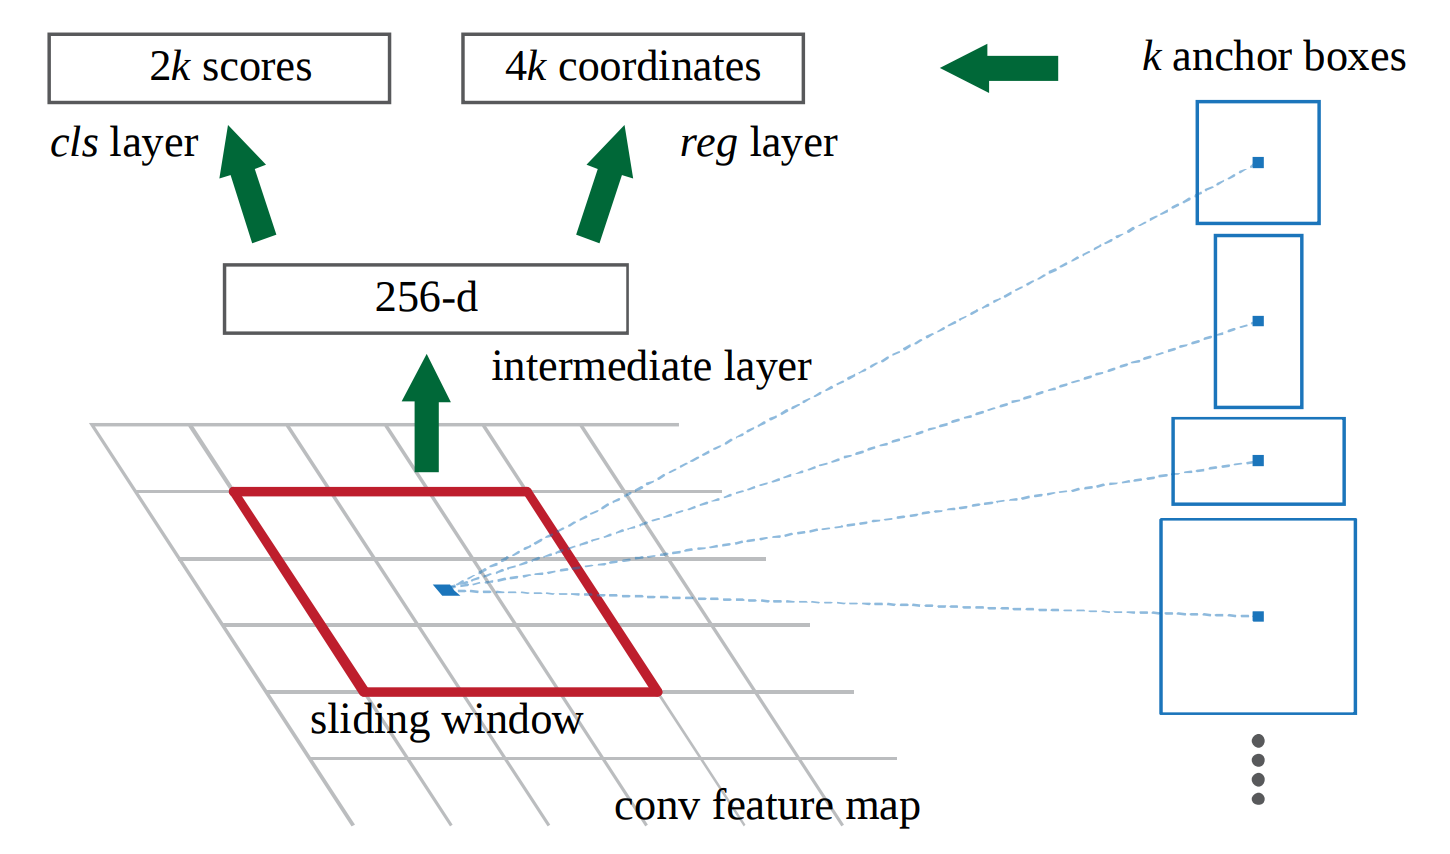
\includegraphics[scale=.5]{image/anchor.PNG}
%     \end{center}
%     \caption{List of all anchors types}
%     \label{ref_chapter2}
%     \end{figure}
% \end{center}
% Anchor: Với mỗi vị trí sliding window, giải thuật sẽ đưa ra N region proposal. Mỗi region tương ứng một trong N loại anchor ở trên. \\

% Kích thước vật lí của mỗi anchor là khác nhau, từ 0.3 mét cho đến 2 mét. Nếu sử dụng single-scale RPN thì sẽ dự đoán tất cả các bao đóng có cùng receptive field. Nên multi-scale RPN đã cho ra những proposal với kích thước nhỏ, lớn khác nhau. Với những proposal kích thước lớn nó có một lớp pooling để tăng receptive field cho những đối tượng lớn hơn. Ở đây những anchor được chia thành 2 level dựa trên kích thước vật lí của nó và sử dụng một nhánh khác của mạng để đưa ra dự đoán cho chúng.\\

% \begin{center}
%     \begin{figure}[htp]
%     \begin{center}
%      \includegraphics[scale=.5]{image/RPN.PNG}
%     \end{center}
%     \caption{3D amodal region proposal network}
%     \label{ref_chapter2}
%     \end{figure}
% \end{center}

% Kiến trúc: Ảnh trên là cho ta trực quan về kiến trúc của mạng. Bước đi (stride) của lớp convolution cuối cùng là 1 tương ứng 0.1 mét trong 3D. Kích thước bộ lọc là 2x2x3 cho level 1 và 5x5x5 cho level 2, chúng tương ứng với 0.4$m^3$ receptive field cho level 1 của những anchor và 1$m^3$ cho level 2 của những anchor lớn hơn.\\

% Với độ phân giải, phạm vi và kiến trúc của mạng thì tổng số anchor là 1,387,646. Trung bình có $92.2\%$ số anchor là rỗng , nó sẽ tự động bị bỏ qua trong quá trình huấn luyện và kiểm tra.\\

% 3D box regression: Mỗi 3D box được biểu diễn tâm điểm của nó $[c_x,x_y,c_z]$ và kích thước của bao đóng là $[s_1,s_2,s_3]$ theo 3 hướng chính của bao đóng. Để huấn luyện 3D box regressor, chúng ta sẽ đoán sự sai biệt của tâm và kích thước giữa anchor và ground truth box. Với mỗi anchor là mẫu dương và grouth truth tương ứng của nó, biễu diễn độ dời của tâm là sự sai biệt $[\Delta c_x,\Delta c_y,\Delta c_z]$ so với hệ tọa độ của máy ảnh. Với sự sai biệt về kích thước thì ta tính độ dời $[\Delta s_1,\Delta s_2, \Delta s_3]$ . Vậy mục tiêu của 3D box regression là một vector có 6 thành phần như sau $ t = [\Delta c_x,\Delta c_y,\Delta c_z,\Delta s_1,\Delta s_2, \Delta s_3]$
% \subsection{Joint Amodal Object Recognition Network}
% \begin{center}
%     \begin{figure}[htp]
%     \begin{center}
%      \includegraphics[scale=.5]{image/ORN.PNG}
%     \end{center}
%     \caption{Joint object recognition network}
%     \label{ref_chapter2}
%     \end{figure}
% \end{center}
%  Sau khi có được những 3D proposal box, không gian 3 chiều cùng với mỗi bao đóng sẽ được cho vào Object Recognition Network (ORN). Theo cách này, những proposal là những bao đóng mà đối tượng nằm hoàn toàn trong đó, ORN có thể vẫn nhận ra kích thước đầy đủ của đối tượng dù có bị ẩn hay dữ liệu bị nhiễu hặc mất mát.\\
 
% 3D ORN: Tất cả các lớp pooling là $2^3$  với stride 2. Với 3 lớp convolution, kích thước của cửa sổ là $5^3$,$3^3$ và $3^3$ tất cả đều có stride là 1. Giữa các lớp fully connected là lớp ReLu và dropout ( hệ số dropout là 0.5).\\

% 2D ORN: Với mỗi 3D proposal box, chúng ta sẽ chiếu những điểm trong proposal box thuộc không gian 3 chiều sang mặt phẳng của ảnh 2 chiều, và lấy bao đóng 2D chứa tất cả những điểm của phép chiếu. Sử dụng mạng VGGnet\cite{VGG} đã huấn luyện sẵn trên ImageNet để trích xuất đặc trưng màu sắc từ ảnh. \\

% 2D và 3D joint recognition: Xây dựng sự kết hợp giữa mạng 2D và mạng 3D để sử dụng cả thông tin về màu sắc và độ sâu. Đặc tính từ VGG Net và 3D ORN sẽ được tổng hợp lại thành một vector đặc tính và cho vào lớp fully connected để giảm số chiều xuống. 2 lớp fully connected sau sẽ lấy kết quả đó để dự đoán nhãn của đối tượng và bao đóng 3D. \\


% \subsection{Kết quả}
% \begin{center}
%     \begin{figure}[H]
%     \begin{center}
%      \includegraphics[scale=.5]{image/table3.PNG}
%     \end{center}
%     \caption{Comparison on 3D object detection}
%     \label{ref_chapter2}
%     \end{figure}
% \end{center}

% Hình 2.4 cho thấy so sánh với 2 phương pháp khác 3D sliding shapes\cite{ss} 
% và 2D Depth-RCNN\cite{guppta}. Kết quả cho thấy sự cải thiện rõ rệt trên tập dữ liệu NYUv2.\\

% \section{DengCVPR 2017\cite{amodal3dobject}}
%  Đây là một công trình gần đây đạt được kết quả khá tốt trong năm 2017 và hứa hẹn sẽ có nhiều cải tiến trong tương lai.\\

% Công trình này nhìn bài toán nhận diện vật thể 3D từ góc nhìn 2D. Một đề xuất mới với mạng neuron nhận diện 3D dựa trên Fast-RCNN\cite{fastrcnn} nó sẽ kết hợp một cách tự nhiên thông tin độ sâu tương ứng với thông tin trên ảnh màu để xác định loại vật thể, hướng và kích thước vật lí. Tại đó bao đóng 2D cùng với ảnh độ sâu sẽ là input.\\



% Nhóm sẽ trình bày chi tiết hơn về công trình này trong phần hướng tiếp cận còn sau đây là những kết quả đạt được của nó. Những thí nghiệm thực hiện trên tập dữ liệu NYUv2 được so sánh với kết quả của deep sliding shape có 19 loại đối tượng khác nhau. Kết quả cho thấy phương pháp này cho chỉ số mAP cao hơn là 4.6$\%$

% \begin{center}
%     \begin{figure}[H]
%     \begin{center}
%      \includegraphics[scale=.5]{image/table4.PNG}
%     \end{center}
%     \caption{Comparison with deep sliding shape}
%     \label{ref_chapter2}
%     \end{figure}
% \end{center}


 


 

\chapter{Các công trình liên quan}

% Hiện nay, số lượng các đối tượng vật thể tồn tại trong cuộc sống là rất nhiều và vô cùng đa dạng. Mỗi loại vật thể lại có đặc điểm riêng về hình dạng, kích thước, đặc trưng riêng. Hơn thế nữa, trong cùng một loại đối tượng thì mỗi vật thể cũng có nhiều biến thể, dẫn tới sự khó khăn rất lớn trong việc xác định một mô hình, kích cỡ cố định của mỗi loại vật thể. \\
Sau đây, nhóm sẽ trình bày những tìm hiểu và nghiên cứu của nhóm về quá trình hình thành và phát triển của các phương pháp dự đoán độ sâu cũng như phát hiện và phân mảnh vật thể mà các nhóm nghiên cứu trong nước và trên thế giới đã thực hiện.

%Với mục tiêu của nhóm là có thể ước lượng được khoảng cách của vật thể từ một ảnh RGB, nhiệm vụ đầu tiên cần phải thực hiện đó chính là biết đối tượng vật thể nằm ở đâu, vị trí nào trong bức ảnh. Do vậy, nhóm quyết định áp dụng các kết quả đã đạt được hiện có về phát hiện, bao đóng, phân mảnh vật thể để có thể cải thiện độ chính xác của việc ước lượng khoảng cách. Dưới đây, nhóm xin trình bày quá trình tìm hiểu, cũng như áp dụng các phương thức để thực hiện phát hiện, bao đóng và phân mảnh vật thể.

\section{Dự đoán độ sâu}
Nhóm đã thực hiện những khảo sát trong nước nhưng nhóm chưa tìm được các công trình có liên quan trong khoảng thời gian cho phép, cho nên những nghiên cứu và công trình dưới đây mà nhóm trình bày thuộc các công trình của các nhóm nghiên cứu quốc tế.\\

Bài toán dự đoán độ sâu từ ảnh nguyên gốc dựa trên stereo vision \cite{sinz2004learning,memisevic2011stereopsis} sử dụng những cặp ảnh của cùng một khung cảnh để tái tạo lại hình dạng trong không gian thực. Nhưng sau đó bài toán được tiếp cận theo các hướng chính như sau:
\subsubsection{Dự đoán độ sâu dựa vào ảnh RGB}
Những phương pháp cổ điển để dự đoán độ sâu từ ảnh RGB chủ yếu dựa trên các đặc trưng được lấy từ bức ảnh một cách thủ công, sử dụng mô hình đồ thị xác suất (problistic graphical model) đưa ra những giả định về hình học của khung cảnh để giải quyết vấn đề \cite{hoiem2005geometric,liu2010single, saxena2006learning, saxena2009make3d}, một trong những công trình đầu tiên bởi Saxena et al. \cite{saxena2006learning}, sử dụng mô hình Markov Random Field (MRF) để suy diễn độ sâu từ những đặc trưng cục bộ cho đến đặc trưng toàn cục được trích xuất từ ảnh. Sau đó họ đã tiến hành mở rộng công trình của mình để tái tạo lại khung cảnh 3 chiều \cite{saxena2009make3d}(3D scene reconstruction). Từ đề tài này, Liu et al. \cite{liu2010single} kết hợp bài toán phân đoạn ngữ nghĩa (semantic segmentation) với bài toán ước lượng độ sâu, tại đó nhãn dự đoán được sử dụng như là ràng buộc thêm để quá trình tối ưu trở nên dễ dàng hơn. Những hướng tiếp cận không tham số (non-parametric) \cite{karsch2014depth, liu2011sift, liu2014discrete, konrad20122d}, với hướng đi này ta sẽ thường so trùng đặc trưng (GIST, HOG) giữa ảnh RGB mà ta muốn có ảnh độ sâu với những ảnh của cơ sở dữ liệu RGB-D, nhằm tìm ra những ảnh tương tự với nó nhất, sau đó dùng ảnh độ sâu của những ảnh này tiến hành sinh ra ảnh độ sâu cuối cùng cho ảnh RGB. Cần chú ý rằng những phương pháp này dựa trên giả định rằng những khung cảnh tương tự nhau thì có phân bố độ sâu cũng tương tự nhau.\\

Gần đây, nhờ những bước tiến lớn của học sâu mà nó đã dẫn dắt hướng nghiên cứu sang sử dụng CNN để ước lượng độ sâu. Bởi vì bài toán này khá tương đồng với bài toán gán nhãn ngữ nghĩa (semantic labeling), nên hầu hết các nghiên cứu đã xây dựng mạng CNN của họ dựa trên những kiến trúc đã chiến thắng trong cuộc thi ImageNet Large Scale Visual Recognition Challenge (ILSVRC) \cite{Imagenet}. Eigen et al. \cite{Eigen2014} là nhóm tiên phong sử dụng CNN để dự đoán độ sâu từ một ảnh đơn, kiến trúc của nhóm này gồm 2 phần chồng lên nhau. Phần đầu gọi là coarse-scale network dựa trên AlexNet \cite{Krizhevsky2012}, nó sẽ dự đoán độ sâu của bức ảnh ở mức toàn cục, sau đó kết quả này được tinh chỉnh ở mức cục bộ bởi fine-scale network. Họ còn tiến hành mở rộng công trình của mình để có thể dự đoán thêm được bề mặt và nhãn (predict surface normal and semantic labeling) với một mô hình sâu hơn dựa trên VGG \cite{Simonyan2014} đó là một kiến trúc 3 thành phần để giải quyết được cả 3 bài toán chỉ từ một bức ảnh đơn \cite{Eigen2015}. Laina et al. \cite{laina2016deeper} và Cao et al. \cite{cao2017estimating} dựa trên Residual Nerual Network (ResNet) \cite{KHe2015} nó đã đứng hạng nhất ở bài toán phân loại và nhận diện của ILSVRC và COCO 2015. Cụ thể Laina et al. \cite{laina2016deeper} đã hồi quy giá trị độ sâu bằng một mạng có kiến trúc bao gồm 2 phần, phần đầu dựa trên ResNet, phần sau nhóm của Laina đã đề xuất các khối Up-convolution và Up-projection để sinh ra ảnh độ sâu có độ phân giải cao. Thay vì hồi quy, Cao et al. \cite{cao2017estimating} đã định hướng bài toán ước lượng độ sâu thành bài toán phân loại có nghĩa là thay vì dự đoán chính xác giá trị độ sâu tại mỗi điểm ảnh thì nhóm của Cao sẽ phân loại xem điểm ảnh có giá trị độ sâu thuộc khoảng nào, kiến trúc mà nhóm của Cao đề xuất cũng gồm 2 phần, phần đầu là mạng CNN dựa trên ResNet để phân loại, kết quả này sau đó được tinh chỉnh bằng cách áp dụng fully connected conditional random field được đề xuất bởi \cite{krahenbuhl2011efficient}.

\subsubsection{Kết hợp cảm biến (sensor fusion)}
Nhằm cải thiện chất lượng của ảnh độ sâu được dự đoán thì ngoài sử dụng ảnh RGB, nhiều nhóm nghiên cứu đã sử dụng thêm thông tin được lấy từ các cảm biến khác. Cụ thể  Macini et al.  \cite{mancini2016fast} đã đề xuất một mạng CNN nhận ảnh RGB và ảnh optical flow tương ứng làm đầu vào để dự đoán khoảng cách. Liao et al. \cite{liao2017parse} thì sử dụng máy quét laze (2D laser scanner) dùng để tạo ra tín hiệu độ sâu (additional reference depth signal) như là đầu vào và đạt được độ chính xác cao hơn khi chỉ sử dụng một mình ảnh RGB. Đặc biệt Ma et al. \cite{Ma2017SparseToDense} đã xem xét sử dụng ảnh độ sâu thưa kết hợp với ảnh RGB để sinh ra ảnh độ sâu dày dựa trên kiến trúc của Laina \cite{laina2016deeper} và kết quả cho thấy khá ấn tượng.\\

Kết thúc phần khảo sát các công trình thực hiện dự đoán độ sâu. Nhóm đã chọn đi theo hướng tiếp cận của Ma \cite{Ma2017SparseToDense} cho phần ước lượng độ sâu của nhóm, chi tiết sẽ được trình bày rõ ở chương 4.



\section{R-CNN} 

\subsection{Mô tả chung}

R-CNN \cite{Girshick2013} thực hiện việc tính toán theo các tầng khác nhau được thể hiện ở hình \ref{fig:rcnn}. Đầu tiên, sẽ khởi tạo các vùng mà sẽ được quan tâm (the regions of interest, RoIs). RoIs chính là các bao đóng các vùng độc lập mà trong nó có thể chứa đối tượng. R-CNN sử dụng Selective Search để tạo ra các RoIs.\\

Tiếp theo, một mạng CNN sẽ được dùng để trích xuất các đặc điểm từng mỗi vùng được đề xuất. Vùng này được co giãn theo tỉ lệ để phù hợp với kích thước input của CNN và được đưa vào mạng. Sau khi mạng CNN trích xuất các đặc điểm từ input, thì những đặc điểm này sẽ được đưa vào SVM để thực hiện việc phân loại.

\begin{center}
   \begin{figure}[H]
   \begin{center}
     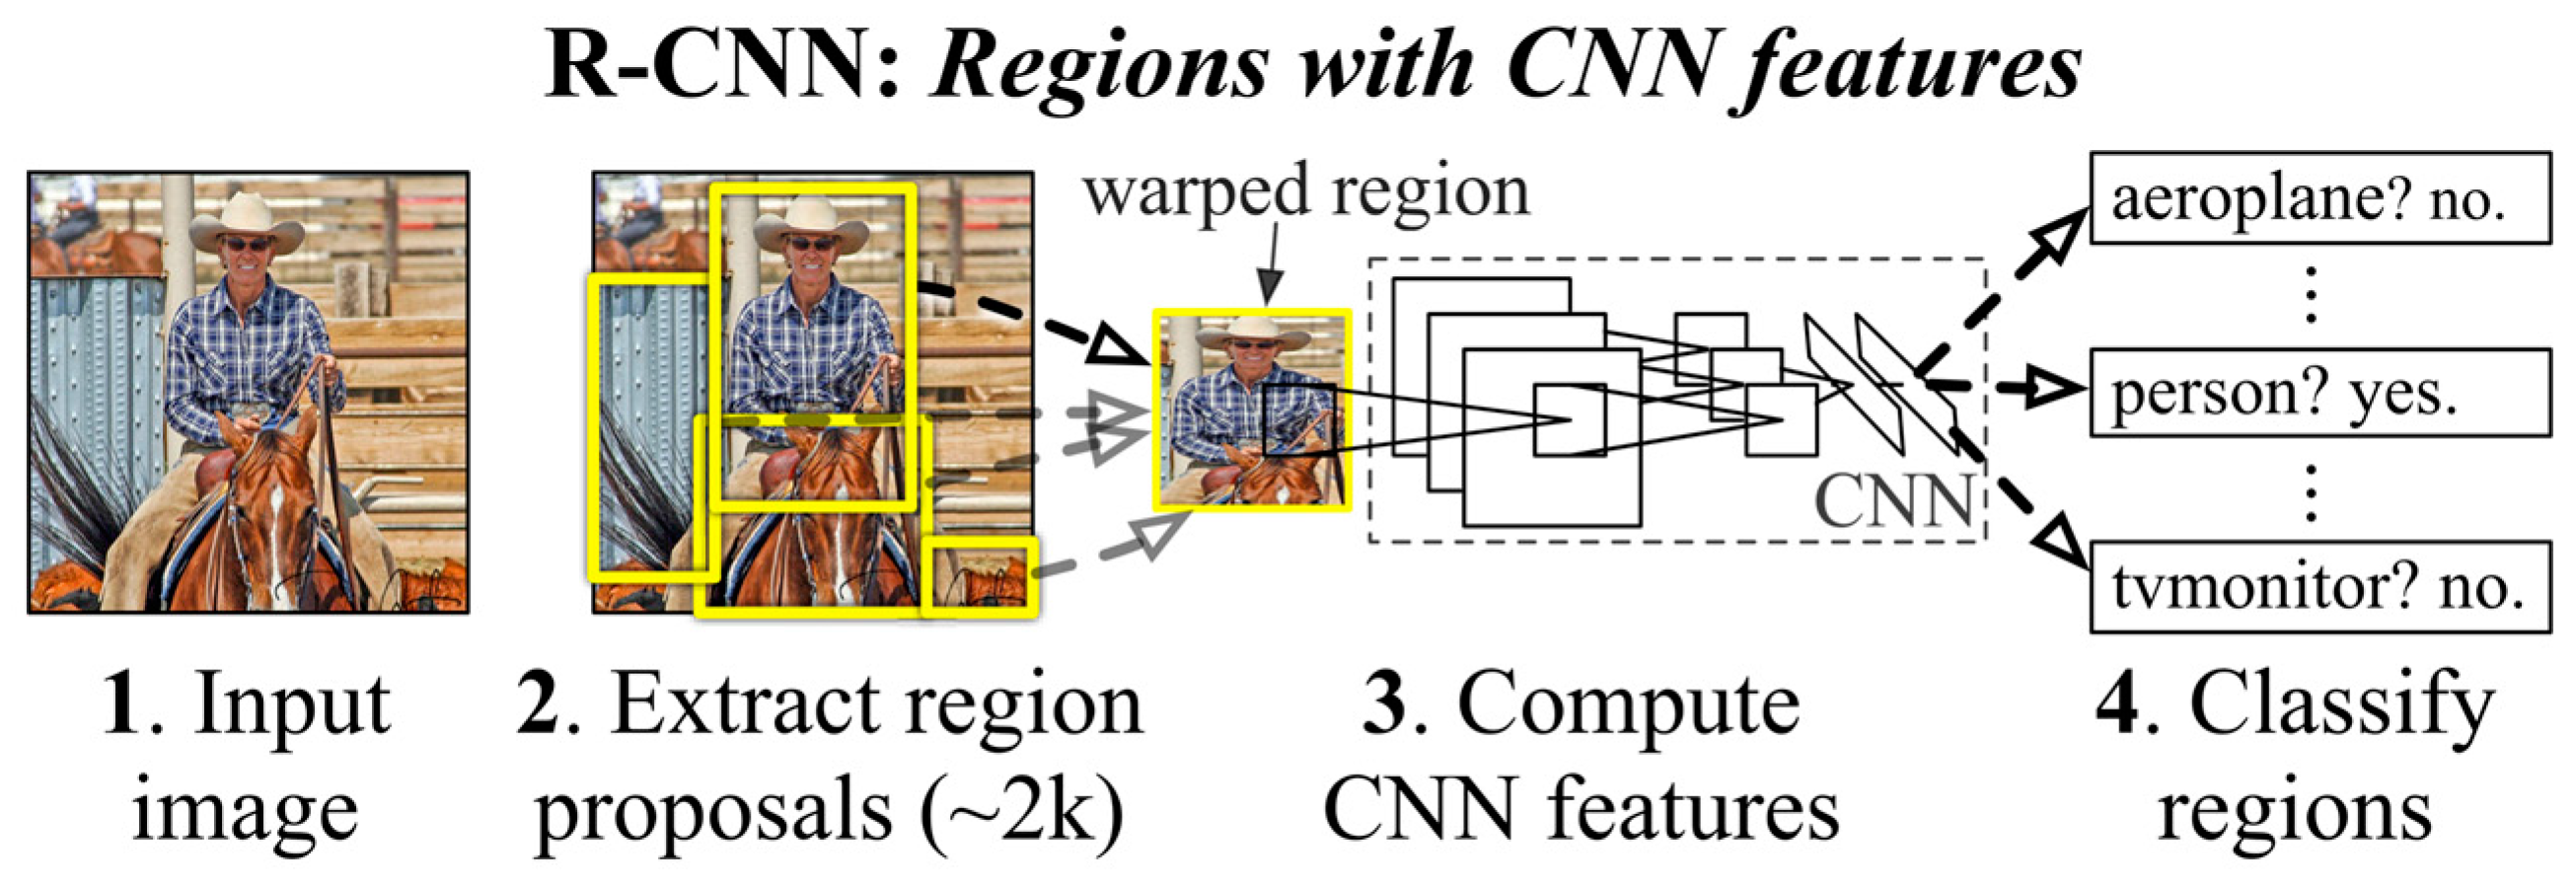
\includegraphics[scale=1.3]{image/rcnn}
    \end{center}
    \caption{Stages of R-CNN}
    \label{fig:rcnn}
    \end{figure}
\end{center}

%Phương thức này được huấn luyện ở nhiều tầng, đầu tiên, mạng %CNN sẽ được huấn luyện. Tiếp theo, SVM sẽ được điều chỉnh dựa %vào các đặc điểm được trích xuất từ mạng CNN. Cuối cùng, %phương thức khởi tạo các vùng được quan tâm được huấn luyện.

\subsection{Hạn chế của R-CNN}

R-CNN là một phương thức nền tảng quan trọng trong phát hiện vật thể, bởi vì nó cung cấp giải pháp đầu tiên cho việc sử dụng CNN cho phát hiện vật thể. Và bởi vì là tiên phong, nên nó có những hạn chế và càng ngày được cải thiện về sau.\\

Những vấn đề chính của R-CNN:
\begin{enumerate}
	\item Quá trình huấn luyện gồm nhiều bước, được mô tả như ở trên.
	\item Với cả việc huấn luyện SVM và phương thức khởi tạo vùng quan tâm, toàn bộ dữ liệu được lưu giữ trên đĩa. Điều này yêu cầu nhiều ngày tính toán cũng như không gian lưu trữ rất lớn.
	\item Cuối cùng, và cũng là quan trọng nhất, việc phát hiện vật thể được thực hiện khá chậm, yêu cầu khoảng một phút cho mỗi ảnh, thậm chí là trên GPU. Bởi vì việc tính toán trên CNN được thực hiện độc lập giữa mỗi vùng được đề xuất,  kể cả những vùng từ cùng một ảnh, có trùng với các vùng khác.
\end{enumerate}

\section{Fast R-CNN} 

Ngay từ cái tên, Fast R-CNN \cite{Girshick2015FastR} đã thể hiện việc nó hình thành dựa trên ý tưởng chính của R-CNN. Nhưng thay vì đưa vào CNN những vùng được đề xuất riêng biệt, thì Fast R-CNN đưa vào mạng CNN toàn bộ bức ảnh để trích xuất đặc điểm.

\subsection{Mô tả chung}

\begin{center}
   \begin{figure}[H]
   \begin{center}
     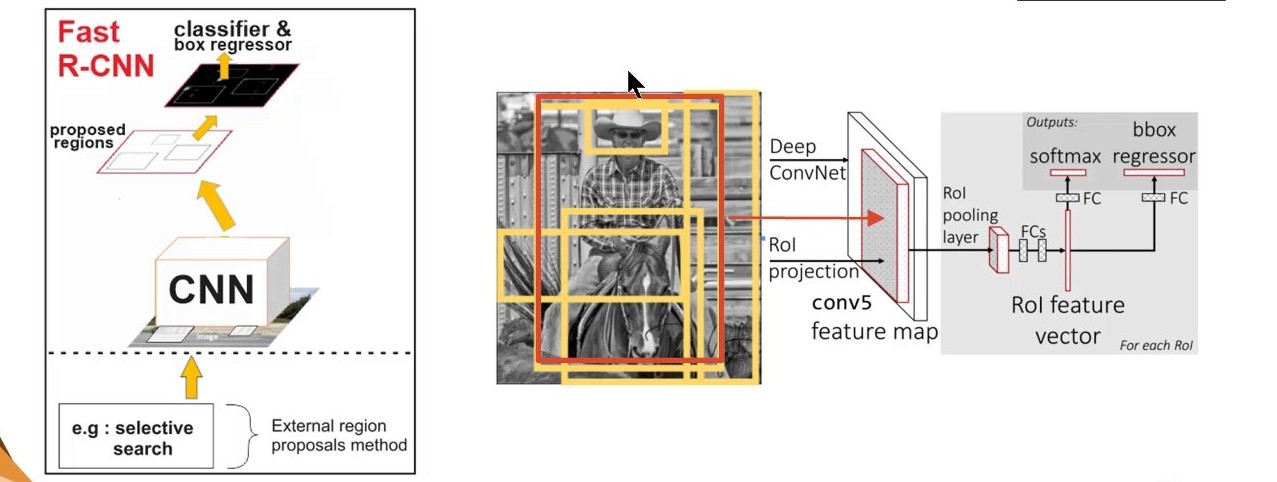
\includegraphics[scale=0.3]{image/fast_rcnn_1}
    \end{center}
    \caption{Stages of Fast R-CNN}
    \label{ref_fast-rcnn}
    \end{figure}
\end{center}

Kiến trúc chung của Fast R-CNN được thể hiện như trên hình 4.1. Fast R-CNN nhận input là bức ảnh và vùng được quan tâm tính toán từ hình ảnh (Region of Interests,RoIs). Cũng giống như R-CNN, thì các RoIs cũng được khởi tạo từ Selective Search, nhưng không phải được thực hiện trên ảnh gốc mà được thực hiện trên feature maps được tạo ra thông qua các lớp convolutional và lớp max-pooling.\\

Khối đặc điểm được trích xuất từ bức ảnh (feature map) kết hợp với các RoIs sẽ là input của lớp RoI pooling. Lớp này có nhiệm vụ tạo ra output có kích cỡ đồng nhất cho mỗi vùng được đề xuất từ feature map. Các vector output từ lớp RoI-pooling sẽ là input của một lớp fully-connected được kết nối với 2 lớp: một lớp softmax để tạo ra xác suất ước tính cho việc phân loại  đối tượng và một lớp bounding-box regressor để ước tính bao đóng cho đối tượng.\\

\subsection{Nhận xét}

Toàn mạng có thể được huấn luyện sử dụng \textit{backpropagation} và \textit{stochastic gradient descent}. Các RoI sẽ được gán nhãn lớp nếu nó giao với bao đóng thật của đối tượng hơn 0.5, ngược lại, những RoI khác sẽ thuộc về lớp nền. Trong việc phân lớp, RoIs từ cùng một ảnh sẽ chia sẻ tính toán và sử dụng bộ nhớ. Theo như kết quả hiện thực, thì Fast R-CNN đã đạt được thời gian ngắn hơn rất nhiều trong trong huấn luyện và test so với R-CNN, cũng như đạt được kết quả tốt hơn trong việc phát hiện vật thể.

\section{Faster R-CNN}

\subsection{Mô tả chung}

Faster R-CNN \cite{Ren2015} là phương pháp nhóm đang nghiên cứu để thực hiện phát hiện vật thể trong không gian 2 chiều. Cũng giống như Fast R-CNN dựa trên nền tảng của R-CNN để đưa ra những cải tiến, thì Faster R-CNN cũng dựa trên Fast R-CNN để đưa ra những thay đổi, hướng tới việc phát hiện vật thể theo thời gian thực. \\

\begin{center}
   \begin{figure}[H]
   \begin{center}
     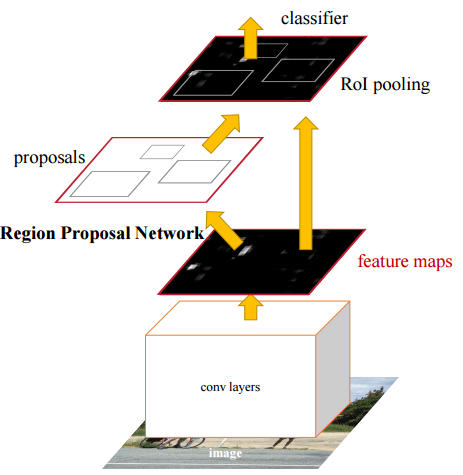
\includegraphics[scale=0.6]{image/faster_rcnn_1}
    \end{center}
    \caption{Faster R-CNN}
    \label{faster_rcnn}
    \end{figure}
\end{center}

Ý tưởng chính của Faster R-CNN là dùng chung các lớp convolutional cho việc khởi tạo các vùng đề xuất và cho việc phát hiện vật thể, ở đây, chính là các feature maps. Sự khác biệt chính giữa Fast R-CNN và Faster R-CNN chính là trong việc khởi tạo các vùng được đề xuất. Với R-CNN và Fast R-CNN, việc khởi tạo các vùng được đề xuất đều sử dụng Selective Search. Với Faster R-CNN, thay vì sử dụng Selective Search, Region Proposal Network được áp dụng và cho thấy được kết quả tốt hơn, không chỉ về chi phí tính toán mà cũng như thời gian thực thi. \\

Mạng CNN sẽ nhận một ảnh vào như là input. Feature maps sẽ được tạo ra từ mạng CNN, và nó được đưa vào như là input của RPN (region proposal network). Output của RPN kết hợp với feature maps sẽ tiếp tục là input của lớp phân loại cuối cùng, lớp này hình thành theo cấu trúc của Fast R-CNN. \\

Do sự chia sẻ kết quả feature map từ các lớp convolutional cho  việc khởi tạo các vùng được đề xuất, nên thời gian tính toán cũng như hiệu quả tính toán được cải thiện khá nhiều.

\subsection{Region Proposal Networks}
Như đã được đề cập nhiều ở trên, RPN nhận một ảnh là input và output chính là một tập các vùng được đề xuất có thể chứa đối tượng.Với convolutional feature map chúng ta có được sau khi đưa ảnh qua mạng convolutional ban đầu, sử dụng cửa sổ trượt với kích cỡ nxn trên feature map nhận được.\\

\begin{center}
   \begin{figure}[H]
   \begin{center}
     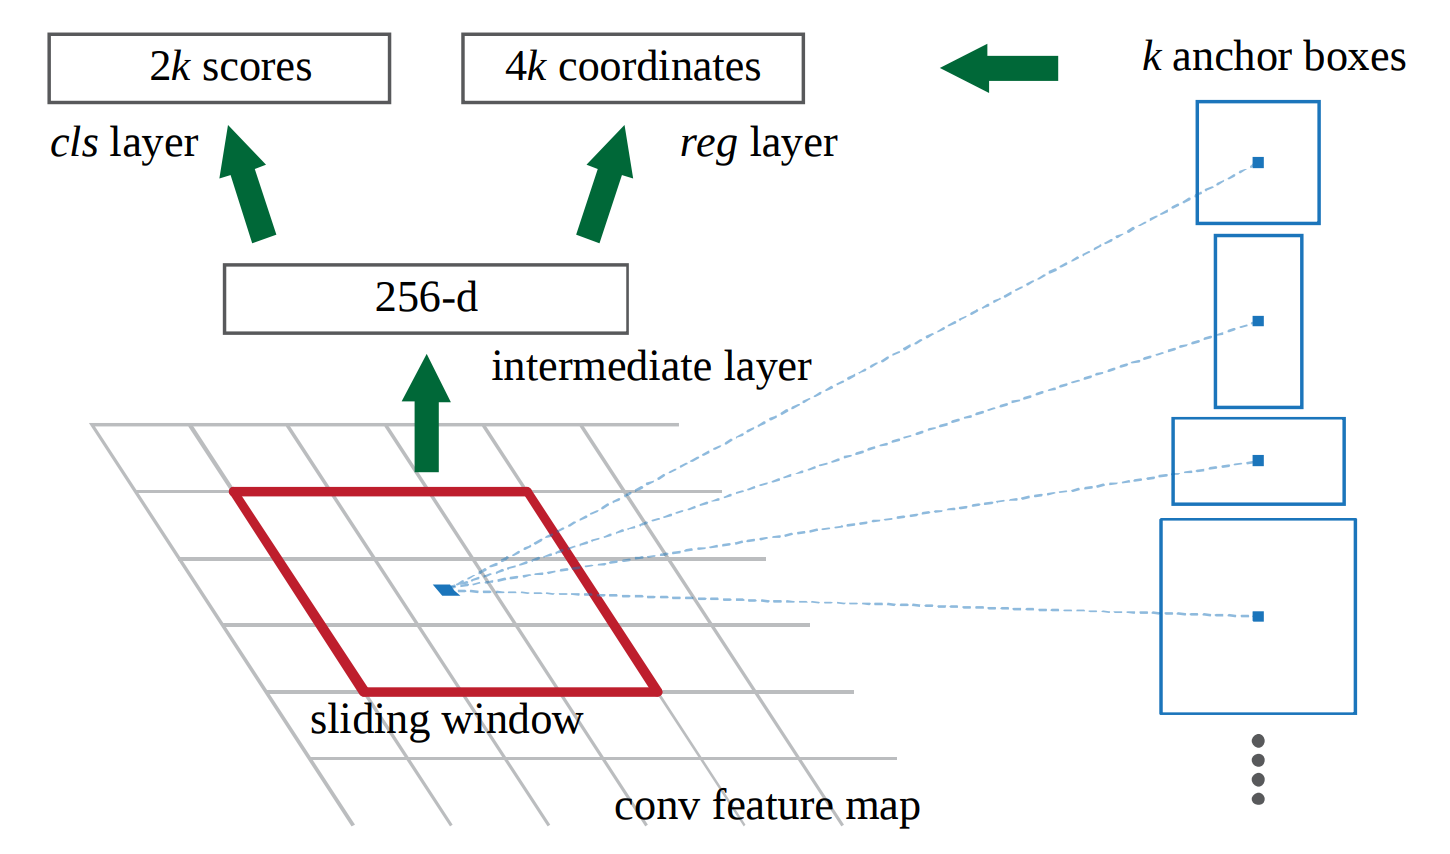
\includegraphics[scale=0.25]{image/anchor}
    \end{center}
    \caption{Region Proposal Network}
    \label{RPN}
    \end{figure}
\end{center}
Tại mỗi vị trí của cửa sổ trượt, Faster R-CNN đưa ra nhiều vùng đề xuất, và  số  những vùng với xác suất cao nhất có thể chứa vật thể tại mỗi vị trí là k. Do vậy, với lớp \textit{reg} sẽ có 4k output đại diện cho vị trí của vùng được đề xuất đó, và lớp \textit{cls} sẽ có output là 2k điểm ước tính xác suất có hoặc không có vật thể trong mỗi vùng đề xuất. Mỗi vùng trong k vùng được đề xuất ở trên được gọi là anchor. Mỗi anchor được đặt tại chính giữa ở mỗi của sổ trượt, và được phối hợp với tỉ lệ thu phóng (scale), và tỉ lệ cạnh (aspect ratio) nhất định. Mặc định, Faster R-CNN sử dụng 3 tỉ lệ thu phóng và 3 tỉ lệ cạnh, do đó k=9 anchors tại mỗi cửa sổ trượt.

% \begin{center}
%    \begin{figure}[htp]
%    \begin{center}
%      \includegraphics[scale=0.5]{image/anchor_1}
%     \end{center}
%     \caption{Anchor}
%     \label{ref_sigmoid}
%     \end{figure}
% \end{center}

\subsection{Nhận xét}

\begin{center}
   \begin{figure}[H]
   \begin{center}
     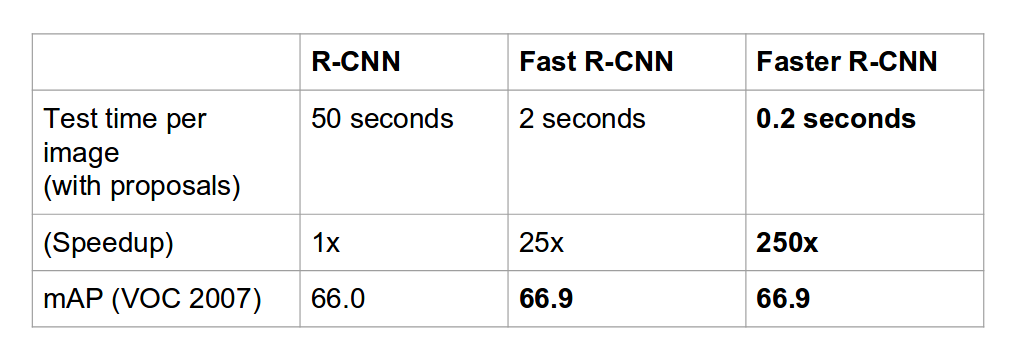
\includegraphics[scale=0.4]{image/fasterrcnn_result}
    \end{center}
    \caption{Faster R-CNN result}
    \label{ref_fasterrcnn_result}
    \end{figure}
\end{center}

Faster R-CNN cho thấy sự hiệu quả trong việc phát hiện vật thể khi thực hiện trong thời gian 200ms/1 ảnh, nhỏ hơn rất nhiều Fast R-CNN với thời gian 2s/1 ảnh. Faster R-CNN đã hướng đến phát hiện vật thể trong thời gian thực, phục vụ những nhu cầu hiện nay.\\

Ngoài ra, không chỉ Faster R-CNN, cũng có rất nhiều phương thức thực hiện việc phát hiện vật thể hiệu quả, nhanh chóng như SSD, YOLO ...\\


\section{Mask RCNN}

Dựa trên cấu trúc Faster RCNN, Mask RCNN \cite{He2017MaskR} ra đời đã cho kết quả rất tốt trong nhiệm vụ phân đoạn vật thể. Mask RCNN đã sử dụng ResNet, Feature Pyramid Network (FPN) nhằm trích xuất đặc điểm từ ảnh, đây là một trong những yếu tố quan trọng giúp Mask RCNN đạt được kết quả cao cả về tốc độ, lẫn độ chính xác. Với việc kết hợp sử dụng ResNet và FPN, thì mô hình đã có những feature maps rất tốt, để thực hiện bao đóng và segmengation vật thể. \\


\begin{center}
   \begin{figure}[H]
   \begin{center}
     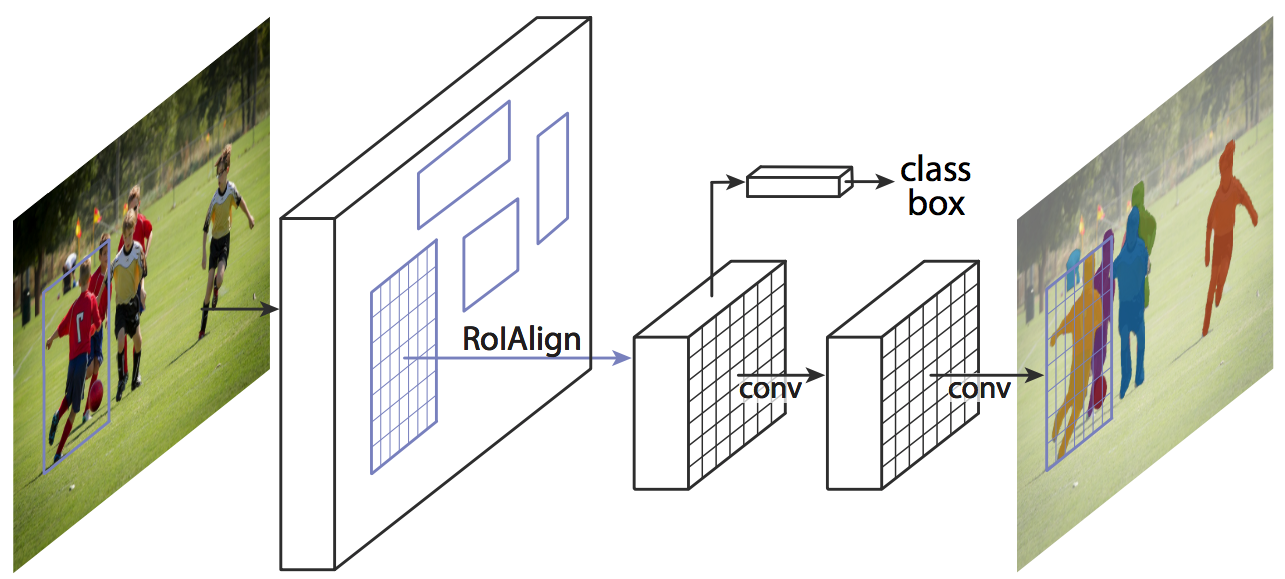
\includegraphics[scale=.2]{image/maskrcnn}
    \end{center}
    \caption{Mask RCNN}
    \end{figure}
\end{center}

Dựa trên kiến trúc của Faster RCNN, Mask RCNN đã thêm một nhánh để thực hiện phân đoạn, độc lập với việc phát hiện, bao đóng vật thể. Để có thể phân loại từng pixel trong ảnh một cách chính xác, Lớp ROIAlign sẽ thay thế cho ROIPool để ko đánh mất thông tin trong featuer map khi trích xuất nó về một feature map nhỏ hơn. Đây cũng là một trong những điểm nhấn, cải tiến quan trọng của Mask RCNN để đạt được những kết quả tốt hơn trong việc phân đoạn. Từ những feature map lấy được, Mask RCNN áp dụng Fully Convolution Network (FCN) để thực hiện việc phân đoạn. 







\chapter{Kiến thức nền tảng}
\section{Học máy}

Học máy được sử dụng rất nhiều trong thị giác máy tính. Trước khi xem xét các nhiệm vụ liên quan đến hình ảnh, nhóm sẽ có một cái nhìn sơ lược về những điều cơ bản trong học máy.\\

Học máy đã xuất hiện như một công cụ hữu ích với khả năng tự học hỏi dựa trên dữ liệu mà không cần phải lập trình cụ thể. Những năm gần đây, khi mà khả năng tính toán của các máy tính được nâng lên một tầm cao mới và lượng dữ liệu khổng lồ được thu thập bởi các hãng công nghệ lớn, học máy đã tiến thêm một bước dài và ngày càng phổ biến với khả năng ngày càng mạnh mẽ.


\subsection{Phân loại các thuật toán học máy}

Theo phương thức học, các thuật toán học máy thường được chia thành các nhóm khác nhau: học có giám sát, học không giám sát, học bán giám sát...\\

\textbf{Học có giám sát} là nhóm phổ biến nhất trong các thuật toán học máy. Nó là thuật toán dự đoán đầu ra của một dữ liệu mới dựa trên các cặp (dữ liệu, nhãn) đã biết từ trước. Ví dụ trong vấn đề nhận diện vật thể, chúng ta sẽ sử dụng dữ liệu đã được đánh dấu vị trí và lớp của các vật thể riêng biệt để huấn luyện. Sau khi học xong, thuật toán có thể dự đoán lớp và vị trí của những dữ liệu mới. \textit{Phân lớp} và \textit{hồi quy} là hai loại chính trong học có giám sát. Trong phân lớp, thuật toán sẽ dự đoán các lớp chính xác của dữ liệu mới dựa trên dữ liệu huấn luyện. Trong hồi quy, thay vì chia thành các nhóm thì đầu ra là một giá trị cụ thể. Gần đây, Microsoft có ứng dụng dự đoán giới tính và tuổi dựa trên khuôn mặt, thì phần dự đoán giới tính có thể coi là thuật toán phân lớp, phần dự đoán tuổi có thể coi là thuật toán hồi quy.\\

Với \textbf{học không giám sát}, chúng ta không biết được outcome hay nhãn mà chỉ có dữ liệu đầu vào. Sau đó, dựa vào cấu trúc dữ liệu để thực hiện một công việc nào đó, có thể là phân nhóm, dự đoán xu hướng của thị trường ... Các bài toán trong học không giám sát cũng được phân loại, trong đó bài toán \textit{phân nhóm} thực hiện việc phân nhóm toàn bộ dữ liệu thành các nhóm nhỏ dựa trên sự liên quan về dữ liệu trong mỗi nhóm. Ngoài ra, còn có bài toán khi chúng ta muốn khám phá quy luật dựa trên nhiều dữ liệu đã cho trước. Chẳng hạn như những khác hàng mua quần thường có xu hướng mua thêm thắt lưng, hay bia sẽ được tiêu thụ nhiều hơn vào thời gian hè..., từ đó tạo ra hệ thống gợi ý khách hàng, thúc đẩy nhu cầu mua sắm.

\subsection{Tính tổng quát}

Bởi vì dữ liệu huấn luyện không thể bao hàm tất cả mọi trường hợp có thể của dữ liệu đầu vào, do đó, thuật toán học phải có tính tổng quát để có thể xử lí các dữ liệu mới. Một mô hình quá đơn giản sẽ không thể tạo ra được kết quả mong muốn với độ chính xác thấp, còn nếu mô hình quá phức tạp có thể dẫn đến tình trạng quá khớp. Do vậy, tính tổng quát của mô hình rất quan trọng trong việc ứng dụng thực tế.\\

Độ hiệu quả của thuật toán có thể được đánh giá dựa trên hàm mất mát(loss). Hàm mất mát được sử dụng để lượng giá giá trị đầu ra với giá trị thực tế là bao nhiêu. Nếu giá trị lỗi lớn, nghĩa là mô hình của chúng ta chưa thực hiện tốt, độ lỗi càng nhỏ càng thể hiện mô hình đang học tốt hơn. Mặt khác, cần phải quan tâm tới tính tổng quát của mô hình như đã nhắc đến ở trên. Mục tiêu trong giai đoạn huấn luyện chính là tìm cực tiểu của hàm mất mát này.

\section{Neural Networks}

Mạng nơ-ron được được phát minh cách đây khá lâu, nhưng mãi đến gần đây nó mới bắt đầu trở nên phổ biến và được sử dụng rộng rãi. Nguyên nhân là do mạng nơ-ron cần có thiết bị tính toán mạnh mẽ và lượng dữ liệu đủ lớn để huấn luyện. Trước kia, công nghệ phát triển chưa đạt đến trình độ để tạo ra những thiết bị hỗ trợ tính toán cao và lượng dữ liệu thu thập được còn quá ít nên đã kìm hãm sự phát phát triển của mạng nơ-ron. Công nghệ ngày càng phát triển theo thời gian, nhu cầu tính toán ngày càng tăng đã tạo động lực thúc đẩy phát minh ra những thiết bị tính toán ngày càng mạnh mẽ. Thế giới ngày càng trở nên số hóa, các thiết bị số ngày một nhiều, do đó đã góp phần tạo nên một lượng dữ liệu rất lớn. Chính hai điều kiện trên đã góp phần tạo điều kiện cho mạng nơ-ron ngày nay trở nên phát triển và khá phổ biến dưới cái tên "deep learning" nhằm nhấn mạnh những kiến trúc sâu được tạo ra bằng cách chồng các lớp lên nhau.

Mạng nơ-ron là giải thuật học máy được sử dụng nhiều. Và nó cũng là nền tảng để nghiên cứu giải quyết bài toán phát hiện vật thể trong không gian 2 hiều, vì cho đến hiện nay, các mô hình tốt nhất vẫn sử dụng kiến thức từ mạng nơ-ron nhiều lớp. Mạng nơ-ron ngày nay được ứng dụng khá rộng rãi trong nhiều lĩnh vực như thị giác máy tính, nhận diện giọng nói, xử lí ngôn ngữ tự nhiên.Đầu tiên, chúng ta sẽ tìm hiểu cách hoạt động của mạng nơ-ron.

\subsection{Nơ-ron nhân tạo}

Mạng nơ-ron ban đầu được gọi là mạng nơ-ron nhân tạo, bảo vì chúng đã được phát triển dựa trên chức năng thần kinh của bộ não con người. Nghiên cứu tiên phong là của 2 nhà khoa học McCulloch và Pitts. 

\begin{figure}[H]%
    \centering
    \subfloat[A biological neuron]{{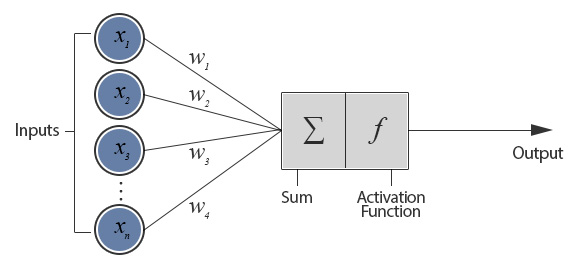
\includegraphics[height=4cm,width=6cm]{image/chapter3_ann} }}%
    \qquad
    \subfloat[Artificial neuron]{{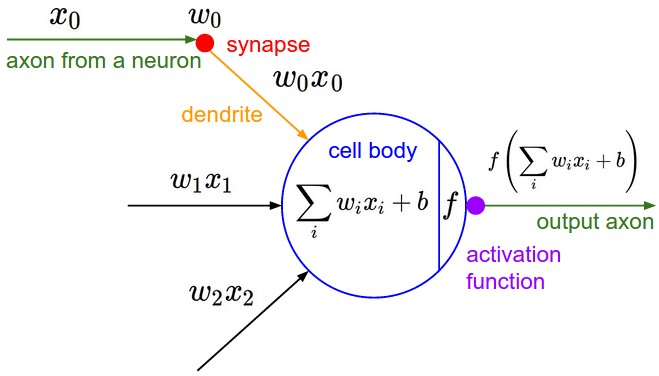
\includegraphics[height=4cm,width=6cm]{image/chapter3_ann_2} }}%
    \caption{A cartoon drawing of a biological neuron (left) and its mathematical model (right).}%
    \label{fig:neuron}%
\end{figure}



Một nơ-ron nhân tạo dựa trên mô hình của McCulloch-Pitts được thể hiện trên hình \ref{fig:neuron}. Nơ-ron nhận n đầu vào với các tham số $x_1, x_2, ...x_i$. Nơ-ron cũng có n trọng số $w_1, w_2, ...w_i$. Những trọng số này thường có một bias với giá trị cố định. Các giá trị đầu vào của nơ-ron kết hợp tuyến tính với các trọng số và được tính tổng lại. Tổng đó sẽ được đưa vào như là input của hàm kích hoạt $f$ (\textbf{activation function}) và tạo ra giá trị output của nơ-ron. Trong lịch sử, lựa chọn phổ biến cho hàm kích hoạt đó là hàm \textbf{sigmoid}, nó lấy input (tổng của các tín hiệu được truyền tới) và nén lại để output sẽ nằm giữa khoảng từ 0 đến 1. Ý tưởng chính ở đây là các giá trị trọng số có thể học được, dựa vào đó đưa ra ouput phù hợp với mỗi input.\\

\begin{center}
	\begin{equation}
		y = f(s) = f(\displaystyle \sum_{i=1}^n(w_ix_i+b_i))
	\end{equation}
\end{center}

Một nơ-ron đơn giống như là một phân loại tuyến tính. Chúng ta có thể thấy với nó sẽ "thích" (kết quả của hàm kích hoạt sẽ gần bằng 1) hoặc "không thích" (kết quả của hàm kích hoạt sẽ gần bằng 0) với giá trị input cụ thể. 

\subsection{Activation function types}

Hàm activation $f$ sẽ nhận vào một số và thực hiện tính toán để xác định output của mỗi nơ-ron. Do vậy, việc chọn hàm activation là quan trọng để có thể tạo ra một mạng hiệu quả. Các nhà nghiên cứu đã sớm nhìn thấy  các nơ-ron và các hệ thống tuyến tính khác sẽ không thể giải quyết được các bài toán không khả phân, ví dụ như bài toán XOR.  Việc thêm nhiều lớp tuyến tính cũng sẽ không thay đổi được vấn đè, bởi vì một mạng kết hợp của nhiều nơ-ron tuyến tính thì nó vẫn duy trì tính tuyến tính. \\

Do vậy, cách đơn giản và hiệu quả để tạo ra một mạng phi tuyến chính là chọn hàm activation phi tuyến. Các hàm activation thường được dùng như  \textit{hàm sigmoid, hàm tanh, hàm ReLU (rectified linear units)}.\\

\begin{center}
   \begin{figure}[htp]
   \begin{center}
     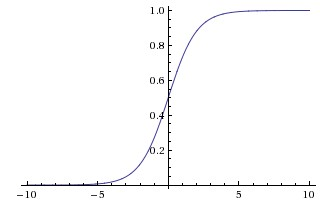
\includegraphics[scale=.5]{image/sigmoid}
    \end{center}
    \caption{Sigmoid function}
    \label{fig:sigmoid}
    \end{figure}
\end{center}

\textbf{Sigmoid}: Sigmoid là một hàm phi tuyến và có công thức toán học: \textbf{$\phi(x) = \dfrac{1}{1+e^x}$} với đạo hàm $f'(x) = f(1-f)$ với đồ thị được thể hiện ở hình trên. Theo như đã nói trước đây, hàm sigmoid sẽ nhận giá trị input và nén chúng thành những giá trị nằm trong khoảng 0 và 1.Trên thực tế, những số âm rất lớn sẽ trở thành 0, những số dương rất lớn sẽ trở thành 1. Do vậy, gần đây hàm sigmoid hiếm khi được sử dụng với các nhược điểm:
\begin{itemize}
	\item Sigmoid mang tính bão hòa và sẽ triệt tiêu đạo hàm. Một thuộc tính không mong muốn của sigmoid đó là khi giá trị của nó tiến về gần 0 hoặc 1, thì đạo hàm tại những vùng đó hầu hết sẽ là 0. Vì trong quá trình backpropagation (sẽ nói đến sau), giá trị đạo hàm này sẽ được nhân với đạo hàm của ouput cho toàn bộ cổng ra. Do đó, nếu giá trị đạo hàm tại đây quá nhỏ, nó sẽ triệu tiêu đạo hàm và hầu như sẽ không có tín hiệu nào được truyền đi, như vậy việc học để cập nhật trọng số sẽ không được thực hiện.
	\item Giá trị của hàm sigmoid sẽ không zero-centered. Nghĩa là nếu giá trị input đến nơ-ron là luôn dương (x>0 với mọi phần tử trong $f = w^Tx+b)$ thì đạo hàm của trọng số $w$ trong suốt quá trình backpropagation sẽ luôn cùng âm hoặc cùng dương. Điều này có thể sẽ dẫn đến việc zig-zaging trong quá trình cập nhật trọng số.
	\item Chi phí tính toán khá lớn.
	
\end{itemize}

\begin{center}
   \begin{figure}[htp]
   \begin{center}
     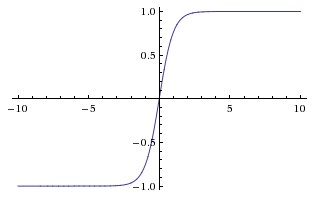
\includegraphics[scale=.5]{image/tanh}
    \end{center}
    \caption{Tanh function}
    \label{fig:tanh}
    \end{figure}
\end{center}

\textbf{Tanh}. Hàm tanh phi tuyến được thể hiện ở hình trên với công thức $tanh(x)=\dfrac{1-e^{-2x}}{1+e^{-2x}} $. Nó sẽ nén các giá trị vào khoảng [-1,1]. Cũng giống như sigmoid nơ-ron, nó cũng sẽ mang tính bão hòa và triệt tiêu đạo hàm. Chi phí tính toán của hàm tanh cũng khá lớn.

\begin{center}
   \begin{figure}[htp]
   \begin{center}
     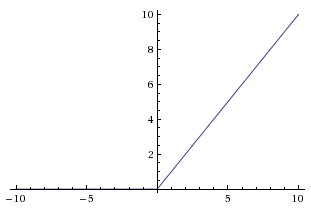
\includegraphics[scale=.5]{image/relu}
    \end{center}
    \caption{ReLU function}
    \label{fig:tanh}
    \end{figure}
\end{center}

\textbf{ReLU}. Hiện nay, hàm ReLU trở nên khá phổ biến, được tính theo công thức $f(x)=max(0,x)$. Với hàm ReLU:
\begin{itemize}
	\item Nó tăng rất nhiều tốc độ tính toán và sự hội tụ của hàm tối ưu nếu so sánh với hàm sigmoid, tanh.
	\item Nếu so sánh về chi phí tính toán của hàm sigmoid, tanh thì hàm ReLU được thực hiện một cách đơn giản, với chi phí thấp.
	\item Ngược lại, sẽ có các thành phần có thể chết và không thể hồi phục trong quá trình luyện. Nếu có một giá trị đạo hàm lớn thì một nơ-ron ReLU có thể làm cho trọng số của phần tử lớn nhất sẽ được cập nhật, còn lại sẽ không bao giờ được cập nhật với bất kì dữ liệu nào nữa. 
\end{itemize}

Vẫn còn nhiều hàm kích hoạt nhưng nhóm chỉ chủ yếu tìm hiểu các loại trên.

\subsection{Multi-layer networks}

\begin{center}
    \begin{figure}[htp]
    \begin{center}
     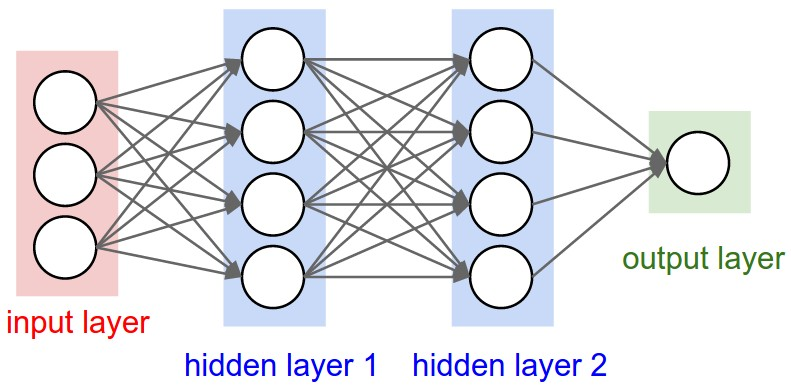
\includegraphics[scale=.4]{image/neural_net2}
    \end{center}
    \caption{A 3-layer neural network}
    \label{fig:multilayer}
    \end{figure}
\end{center}

Mạng nơ-ron là sự kết hợp của nhiều nơ-ron kết nối với nhau. Nói cách khác, thì giá trị đầu ra của một vài nơ-ron sẽ là giá trị đầu vào của những nơ-ron khác. Thay vì một kiến trúc vô định hình các kết nối của các nơ-ron, mạng nơ-ron thường được tổ chức thành các lớp phân biệt của các nơ-ron với nhau. Đối với một mạng nơ-ron thông thường, thì kiểu thường thấy sẽ là fully-connected đối với các nơ-ron giữa hai lớp kề nhau, nhưng những nơ-ron trong cùng một lớp sẽ không có kết nối với nhau. Tính chất của lớp fully-connected là mỗi nơ-ron có số trọng số bằng với số nơ-ron của lớp đứng liền trước nó.\\

Một multi-layer network điển hình bao gồm 3 kiểu lớp, lớp đầu vào, lớp ẩn (hidden layer) và lớp output. Lớp đầu vào thường chỉ truyền dữ liệu đi và không sửa đổi nó. Hầu hết quá trình tính toán xảy ra tại các lớp ẩn. Cuối cùng, lớp đầu ra chuyển giá trị từ các hàm activation của lớp ẩn thành output mong muốn, chẳng hạn là kết quả phân lớp. Một multi-layer network sẽ có ít nhất một lớp ẩn để thực hiện việc tính toán.\\

\subsection{Backpropagation}

Một mạng nơ-ron được huấn luyện chính là việc chọn lựa các trọng số cho tất cả các nơ-ron có trong mạng , từ đó đạt được xấp xỉ các mục tiêu giá trị đầu ra từ những đầu vào đã biết. Việc tìm các trọng số phù hợp của một mạng multi-layer là một công việc khó. Và giải thuật lan truyền ngược(backpropagation) chính là giải pháp phù hợp và hiệu quả để tìm các trọng số. Backpropagation cổ điển sử dụng phương pháp gradient descent như là hàm tối ưu. Gradient descent có thể tốn khá nhiều thời gian và không đảm bảo sẽ tìm được cực tiểu toàn cục của hàm mất mát (loss function), nhưng với việc điều chỉnh phù hợp, nó đủ tốt để có thể ứng dụng trong thực tế.\\

Trong giai đoạn đầu, vector input sẽ được truyền qua mạng nơ-ron, gọi là feedforward. Trước đó, các trọng số của mạng nơ-ron sẽ được khởi tạo giá trị. Output nhận được của mạng nơ-ron sẽ được so sánh với output thật sự, được biết trước ở dữ liệu huấn luyện, bằng việc sử dụng hàm mất mát. Đạo hàm của hàm mất mát sẽ được tính và cũng có thể gọi là giá trị lỗi. Khi sử dụng \textbf{mean squared error (MSE)} như là hàm mất mát, thì giá trị lỗi được hiểu đơn giản là sự khác biệt giữa output hiện tại và output thật sự. \\

Giá trị lỗi sẽ được lan truyền ngược lại trong mạng để tính giá trị lỗi tại các lớp ẩn, gọi là lan truyền ngược(backpropagation). Giá trị lỗi tại các lớp ẩn có thể được tính bằng cách vận dụng đạo hàm của hàm hợp. Cuối cùng, các trọng số của mạng sẽ được cập nhật bằng việc trừ đi một lượng dựa vào tốc độ học (learning rate). Learning rate có thể được đặt cố định hoặc động. Sau khi các trọng số được cập nhật, thuật toán sẽ thực thi lại với dữ liệu đầu vào còn lại trong tập dữ liệu huấn luyện đến khi việc cập nhật trọng số không gây ảnh hưởng nhiều đến giá trị của nó hoặc  dựa vào số lượng dữ liệu trong tập huấn luyện. \\

Trong mô tả ở trên, việc cập nhật các trọng số $w$ sẽ được thực hiện sau mỗi input mới. Còn nhiều cách để có thể thực hiện cập nhật $w$ và trong đề cương luận văn này, nhóm sử dụng mini-batch learning, sử dụng một phần dữ liệu của tập huấn luyện cho mỗi lần cập nhật trọng số.

\subsection{Optimization}

Trong quá trình huấn luyện, việc chênh lệch giữa đầu ra của mô hình và giá trị thực tế là quan trọng. Cải thiện việc chênh lệch giữa 2 giá trị này là mục tiêu của việc huấn luyện. Việc tính toán giá trị chênh lệch này được thực thi bởi hàm mất mát. Tùy theo mục đích của bài toán mà chúng ta có thể lựa chọn hàm mất mát khác nhau.\\

Hàm mất mát sẽ cho chúng ta biết chất lượng của các trọng số, nghĩa là nếu các trọng số ngày càng tốt, thì giá trị của hàm mất mát sẽ ngày càng giảm. Do vậy, mục tiêu cuối cùng của việc tối ưu ở đây chính là tìm các trọng số \textbf{W} sao cho giá trị của hàm mất mát là nhỏ nhất có thể. Có nhiều chiến lược để có thể tối ưu hàm mất mát.
\begin{enumerate}
	\item \textbf{Tìm kiếm ngẫu nhiên}: một cách đơn giản để có thể tìm các giá trị trọng số \textbf{W} đó chính là tìm kiếm ngẫu nhiên. Từ việc ngẫu nhiên ra các trọng số, chúng ta chọn bộ \textbf{W} cho giá trị của hàm mất mát là nhỏ nhất. Tất nhiên, đây là một ý tưởng tồi và không cho kết quả tốt.
    \item \textbf{Phân tích đạo hàm}: chúng ta luôn mong muốn trong mỗi lần cập nhật trọng số, thì \textbf{W} sẽ luôn cho một giá trị tối ưu hơn ở hàm mất mát, nghĩa là có thể chủ động điều chỉnh \textbf{W} theo hướng tốt hơn, và đó là \textit{Gradient Descent}. Ý tưởng chính của Gradient Descent chính là việc cập nhật trọng số bằng việc trừ đi một lượng đạo hàm của chính nó theo một tỉ lệ nào đó. Việc đi ngược hướng với đạo hàm khiến nó càng ngày càng tiến tới điểm cực tiểu, tức khi đạo hàm gần bằng 0. Việc tìm điểm cực tiểu toàn cục trong các hàm mất mát thường rất khó khăn hoặc không khả thi, do đó, người ta thường chọn những điểm cho giá trị hàm mất mát tốt và có thể ứng dụng thực tế hơn là cố gắng tìm kiếm điểm tối ưu toàn cục. \\     
\begin{center}
    \begin{figure}[H]
    \begin{center}
     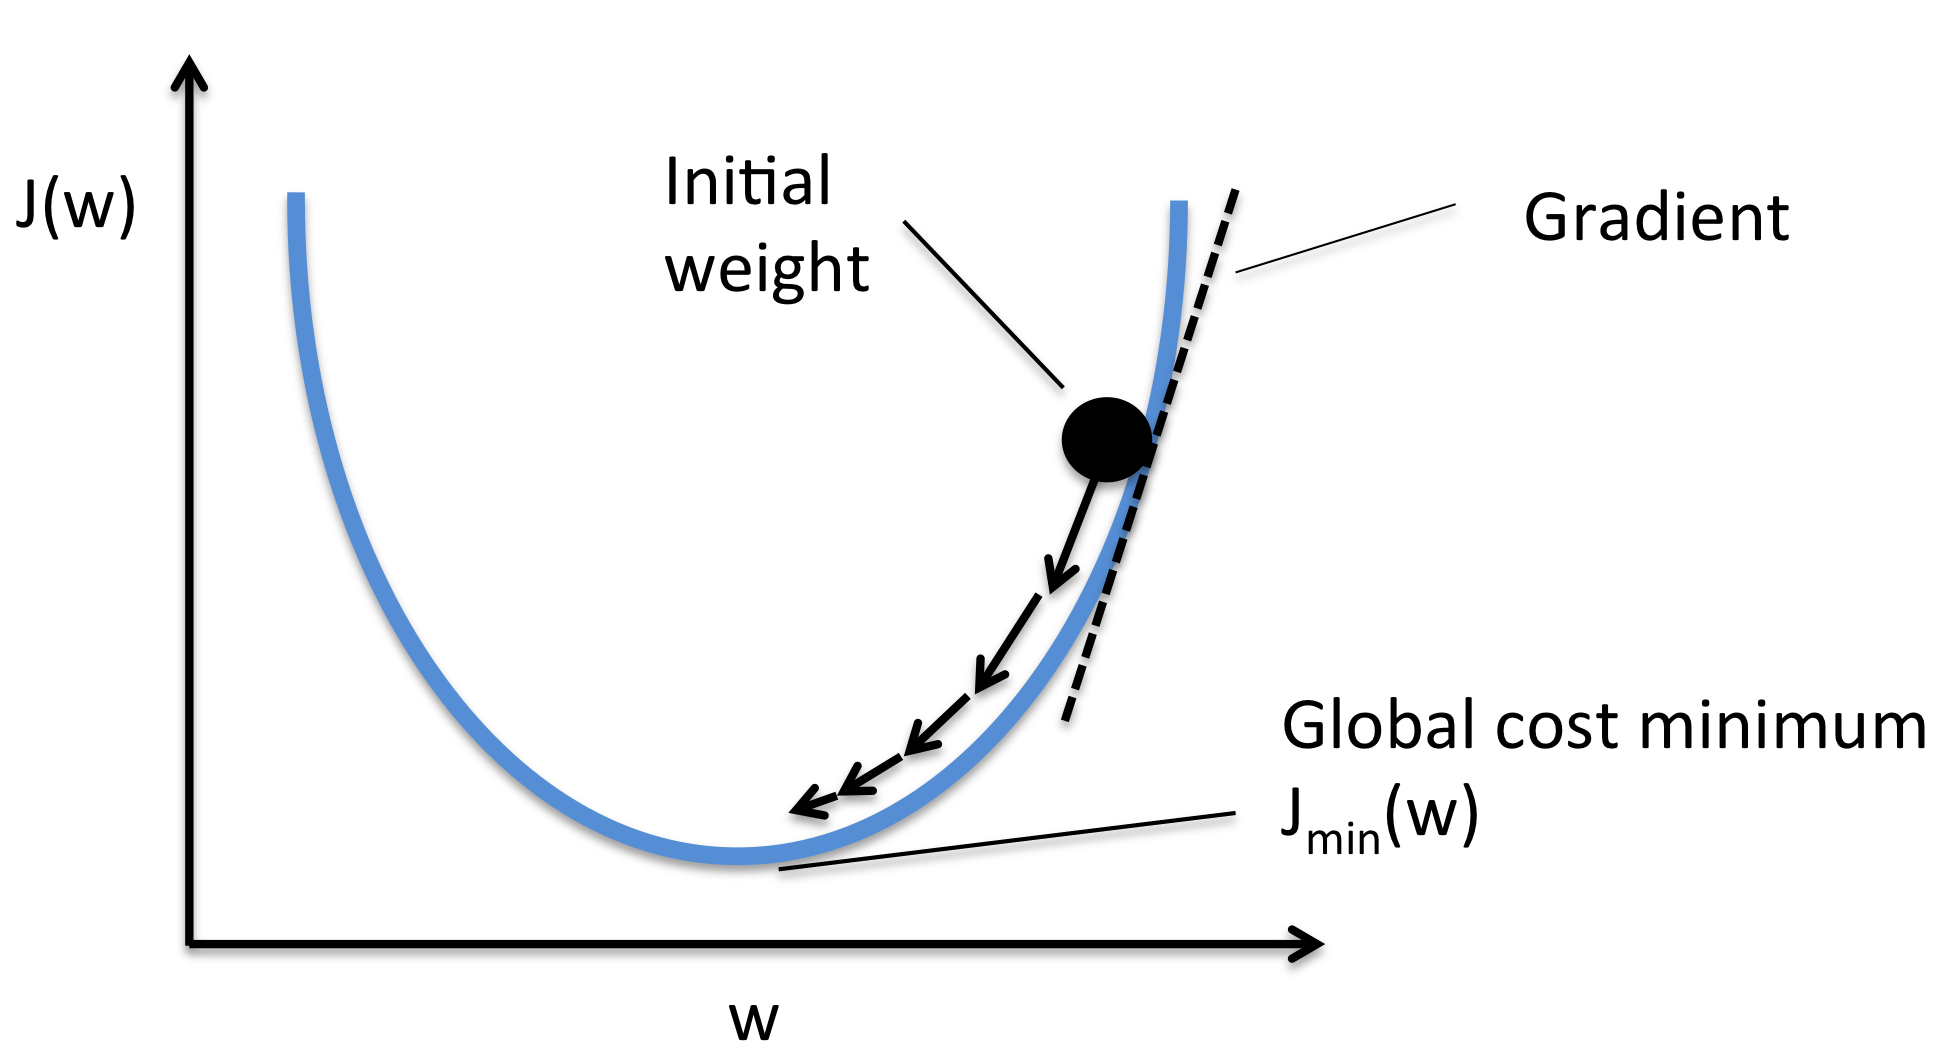
\includegraphics[scale=.15]{image/gradientdescent}
    \end{center}
    \caption{Gradient descent}
    \label{fig:gradientdescent}
    \end{figure}
\end{center}
 
Ngoài ra, trong các ứng dụng quy mô lớn, khi mà tập dữ liệu huấn luyện trở nên rất lớn, ví dụ như hàng triệu ảnh, thì sẽ rất lãng phí nếu chúng ta tính toán hàm mất mát trên toàn bộ tập dữ liệu trong mỗi lần cập nhật trọng số. Các tiếp cận đơn giản cho vấn đề này là chia ra các đợt (batchs) để huấn luyện. Chẳng hạn, mỗi batchs chúng ta sẽ tính toán trên 2 ảnh và thực hiện việc cập nhật trọng số, rồi sẽ thực hiện tiếp trên các batchs còn lại của tập dữ liệu huấn luyện. Phương pháp này chính là \textit{mini-batch gradient descent}
\end{enumerate}

\section{Convolutional neural network}
\subsection{Phân tích}

Với mạng nơ-ron truyền thống, vấn đề trong việc giải quyết các nhiệm vụ trong lĩnh vực thị giác máy tính là một ảnh khiêm tốn cũng sẽ chứa một lượng thông tin khổng lồ.\\

Một ảnh với kích thước 620x480 sẽ có 297600 pixel. Nếu mỗi pixel là mỗi input của một mạng full-connected, mỗi nơ-rơn sẽ có 297600 trọng số. Với một ảnh full HD 1920x1080, một nơ-ron sẽ có 2,073,600 trọng số. Mặc khác, chúng ta có nhiều lớp, do vậy, lượng trọng số chúng ta phải xác định sẽ rất khổng lồ.

\subsection{Kiến trúc cơ bản}
Ý tưởng cơ bản của Convolution neural network(CNN) dựa trên một khái niệm trong sinh học, là vùng thụ cảm (receptive field), hoạt động giống như một cảm biến, chúng nhạy cảm với một số loại kích thích, ví dụ như các cạnh, góc, kiến trúc của các vật thể trong ảnh.\\

ConvNets cũng tương tự như một mạng nơ-ron truyền thống, chúng được cấu thành từ nhiều nơ-ron có khả năng học các trọng số và biases. Mỗi nơ-ron nhận vào một đầu vào(vd:như matrix pixels), thực hiên một phép nhân ma trận sau đó giá trị này sẽ là đầu vào của một hàm phi tuyến. Chức năng sinh học có thể được mô hình hóa bằng máy tính nhờ phép toán chập (convolution operation) .\\

Một CNN thường gỉa định rằng đầu vào là ảnh, điều đó cho  phép chúng mã hóa những đặc tính quan trọng của một bức ảnh nhờ vào kiến trúc của nó. Không giống như mạng neuron thường, các lớp của một ConvNet gồm các nơ-ron được sắp xếp theo 3 chiều: cao, rộng và dài. Thêm vào đó, các nơ-ron trong một lớp chỉ kết nối đến một vùng nhỏ của lớp trước nó, thay cho việc các nơ-ron lớp sau kết nối một cách đầy đủ với các nơ-ron lớp trước như trước đây.\\

Mỗi lớp thực chất chuyển một đầu vào có 3 chiều thành một kết quả 3 chiều với một vài hàm có thể có tham số hoặc không. Phép toán chập của một bức ảnh f và một bộ lọc dưới dạng matrix g được định nghĩa như sau:

\begin{center}
	\begin{equation}
	 h[x; y] = f[x; y] * g[x; y] = \displaystyle \sum_{n}\displaystyle \sum_{m}f[n; m]g[x - n; y - m]
	\end{equation}
\end{center}
\begin{center}
    \begin{figure}[H]
    \begin{center}
     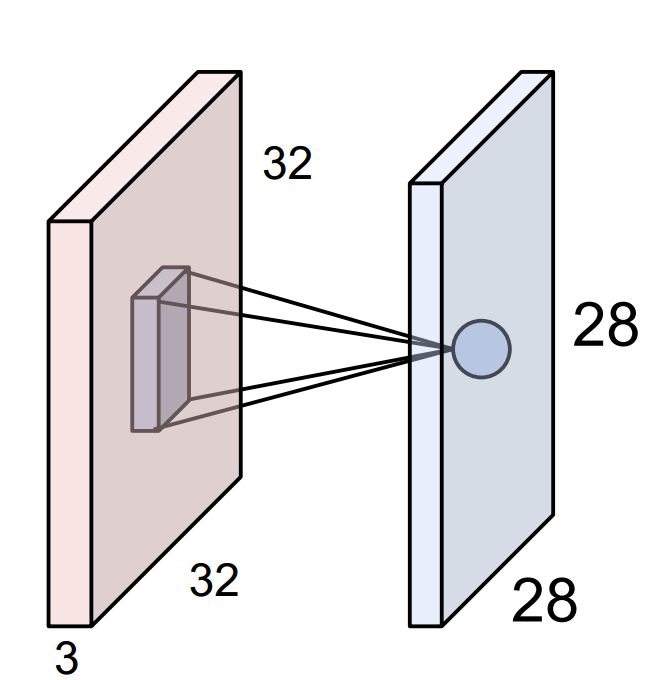
\includegraphics[scale=.5]{image/neuronView.PNG}
    \end{center}
    \caption{}
    \label{fig:conv_operation}
    \end{figure}
\end{center}

Phép toán trên giống như một neuron với bộ lọc g nhìn vào một vùng nhỏ f của lớp trước nó và cho ra một giá trị h tại tọa độ x,y. Kích thước của vùng thụ cảm bị thay đổi bởi kích thước của bộ lọc. Cho bộ lọc chạy dọc theo 2 chiều của bức ảnh để sinh ra một ma trận mới là h. Nó thường được gọi là các trích xuất đặc điểm(feature map) hoặc activation map sau khi h đi qua hàm activation). Nếu ảnh f không có đệm( padding) thì kích thước đầu ra sẽ giảm sau mỗi lần tính phép chập.\\


Một tập hợp các bộ lọc(convolution filter) sẽ tạo thành một lớp convolutional của mạng nơ-ron. Ma trận chứa dữ liệu của filters chính là các trọng số và sẽ được huấn luyện sử dụng các thuật toán học máy. Và các thao tác tích chập này (convolution) sẽ thay thế cho thao tác nhân ma trận ở mạng neuron thông thường. Giá trị đầu ra của lớp convolution giống như hình hộp chữ nhât với chiều sâu bằng số filter. Chiều rộng và chiều cao của khối sẽ giảm so với kích thước ban đầu nếu không được padding.\\

Bởi vì cùng một filter sẽ được sử dụng cho tất cả các phần của bức ảnh, do đó số lượng trọng số sẽ giảm xuống rất nhiều so với mạng fully-connected. Những nơ-ron của một lớp convolutional đều dùng chung một bộ tham số và chúng chỉ kết nối đến một vùng tương ứng trên đầu vào.

\begin{center}
    \begin{figure}[H]
    \begin{center}
     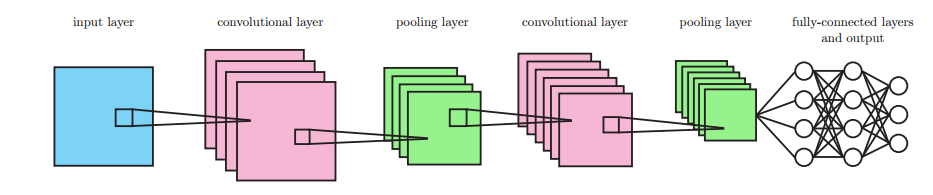
\includegraphics[scale=.5]{image/CNNexample.PNG}
    \end{center}
    \caption{An example of a convolutional network}
    \label{fig:cnn}
    \end{figure}
\end{center}

Ảnh trên là một ví dụ về một mạng ConvNet. Giải thuật lan truyền ngược đã  thảo luận ở trước vẫn được áp dụng. Về mặt lý thuyết, thì những lớp gần input sẽ học được những đặc tính đơn giản của bức ảnh như các cạnh, góc và các lớp sau sẽ tổng hợp những đặc tính học được từ lớp trước để nhận ra những hình dạng phức tap hơn được mô tả như hình bên dưới

\begin{center}
    \begin{figure}[H]
    \begin{center}
     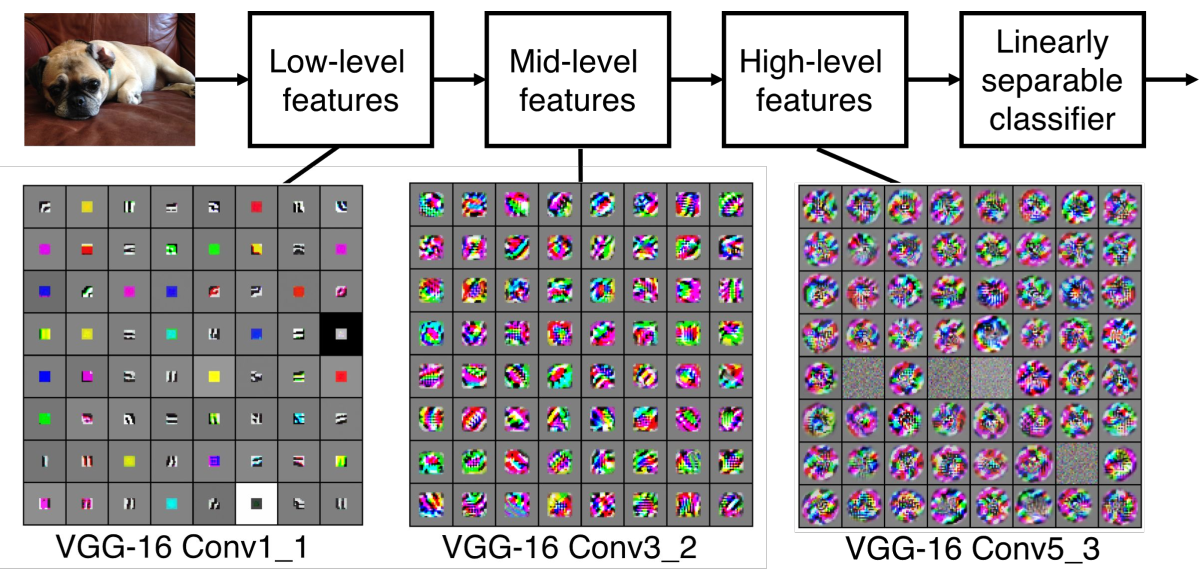
\includegraphics[scale=.5]{image/featureLearning.PNG}
    \end{center}
    \caption{Visualizing the content at each layer}
    \label{fig:visualize_cnn}
    \end{figure}
\end{center}


\subsection{Pooling và stride} 
Với một mạng dùng để phân loại ảnh, một điều cần thiết là nên giảm kích thước của activation map.Thường thì mạng nằm ở nằm sâu phía trong thì cần ít thông tin về đặc tính vị trí, hình dạng mà cần nhiều bộ lọc để có thể nhận ra những mẫu ở mức high-level. Người ta giảm chiều dài và chiều rộng của input volume bằng cách cho nó qua các lớp pooling hoặc tăng bước đi (stride).\\

Với pooling việc giảm kích thước của input volume sẽ giúp giảm số lượng tham số và thời gian tính toán của mạng, qua đó giúp ta kiểm soát hiện tượng over-fitting. Pooling layer tính toán độc lập trên mỗi activation map của một input volume khiến output volume sẽ có cùng chiều sâu với input nhưng chiều rộng với chiều cao đã giảm. Nhưng pooling có thể làm mất đi những thông tin về sự liên hệ đến hình dạng giữa những phần của các mẫu. Phương pháp pooling thông thường là max-pooling đơn giản nó chỉ cho ra giá trị lớn nhất trong hình chữ nhật tương ứng với kích thước bộ lọc mà nó chọn.\\
\begin{center}
    \begin{figure}[htp]
    \begin{center}
     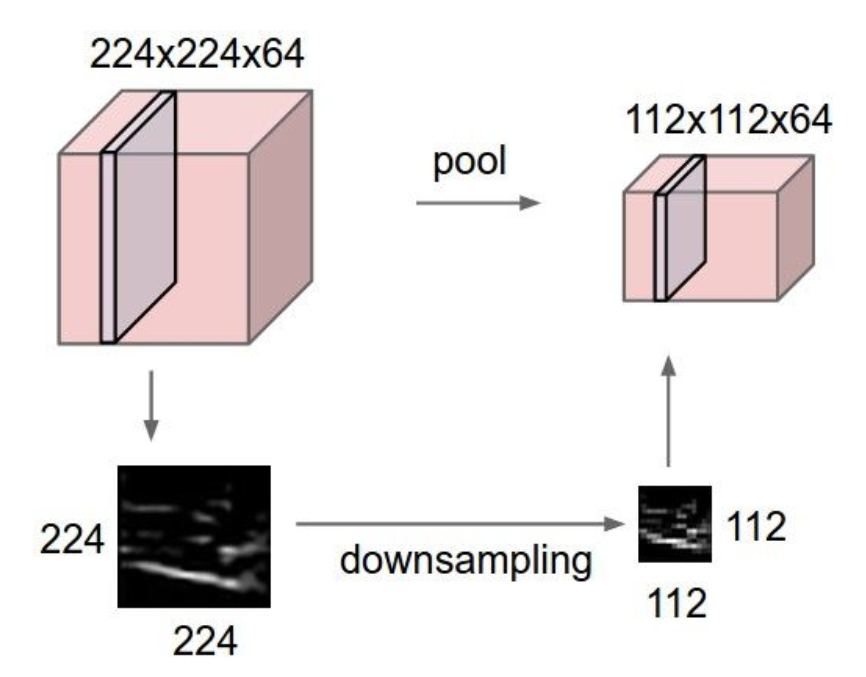
\includegraphics[scale=.5]{image/pooling}
    \end{center}
    \caption{An example of a pooling operation}
    \label{ref_chapter3_cnn}
    \end{figure}
\end{center}

Một cách khác để giảm input volume là tăng bước đi (stride) trong phép chập (vd: stride bằng 1 thì ta sẽ dich chuyển filter tại 1 pixel 1 lần). Theo nhiều nghiên cứu thì người ta không dùng pooling layer mà không mất đi độ chính xác bằng cách chỉ sử dụng nhưng bước đi lớn hơn tại mỗi phép chập.

\subsection{Additional layers}
Lớp convolutional thường có một hàm activation là hàm phi tuyến, như ReLu, thông thường nó được tách ra thành một lớp riêng nằm giữa lớp convolutional và lớp pooling.
Lớp cuối cùng của một ConvNet thường là fully-connected layer.\\

Một lớp fully-connected có thể lấy ra được những liên hệ thú vị của các phần từ input mà lớp convolutional không thể làm được. Tuy nhiên, để lớp này làm việc hiểu quả thì input cho nó phải là một volume có kích thước nhỏ thôi. Pooling và stride như phân tích ở trên sẽ làm giảm kích thước cho phù hợp, rồi mới đưa vào cho lớp này xử lí. Một số mạng không dùng đến fully-connected layer gọi là fully convolutional network (FCN).\\

Nếu mạng sử dụng cho image classification. Thì phần mạng phía trước fully-connected layer hoạt động giống như một bộ lọc, biểu diễn những đặc tính quan trọng, và khi đến lớp này chúng sẽ tổng hợp lại để đánh giá xem input là thuộc mẫu nào.
\begin{center}
    \begin{figure}[htp]
    \begin{center}
     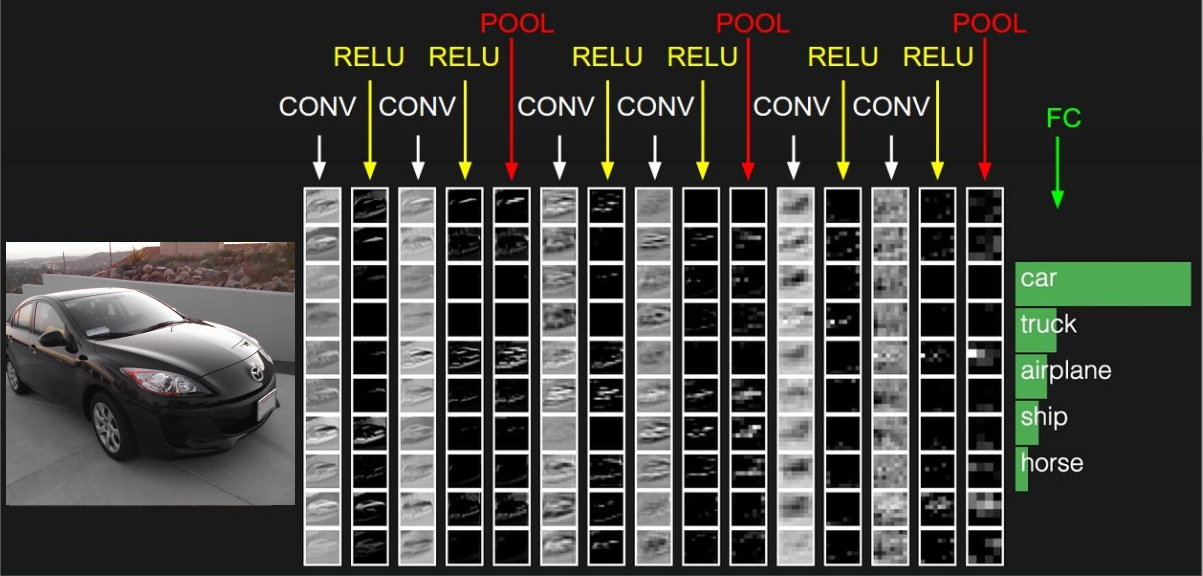
\includegraphics[scale=.5]{image/imageClass}
    \end{center}
    \caption{Classifying an image using a ConvNet}
    \label{ref_chapter3_cnn}
    \end{figure}
\end{center}
\subsection{Regularization}
Để can thiệp vào hiện tượng overfitting người ta thường đưa thêm những ràng buộc hoặc thông tin cho một hệ thống tự học. 
Một cách khá thông thường được sử dụng trọng mạng neuron để giới hạn khả năng của mô hình là thêm một tham số mới vào hàm đo độ lỗi hay hàm mục tiêu, ở đây ta định nghĩa hàm K\cite{DLbook}
\begin{center}
	\begin{equation}
	 K(\Theta;X;y) = J(\Theta;X;y) + \alpha\Omega(\Theta)
	\end{equation}
\end{center}
Nếu $\alpha = 0$ thì sẽ không có chính quy hóa, $\alpha$ càng lớn thì tăng chính quy hóa. Thường hàm K sẽ là hàm lỗi và nếu $\alpha$ lớn nó sẽ khiến cho giá trị của các trọng số học được nhỏ.\\

Dùng chung tham số trong ConvNet cũng là một ví dụ khác của chính quy hóa.
Một cách khác cũng khá phổ biến là dropout. Nó sẽ ngẫu nhiên bỏ đi một số neuron trong quá trình huấn luyện bằng việc thiết lập những giá trị tại đây là 0, nó sẽ tạo ra một mạng khác một ít so với ban đầu. Điều này sẽ khiến cho hệ thống không phụ thuộc quá nhiều vào số kết nối hoặc mỗi neuron, do đó giúp tính toán hiệu quả hơn. Trong ConvNet thì dropout thường sử dụng ở fully-connected layer.\\

Overfitting còn có thể được giảm bằng cách tăng số lượng của tập dữ liệu huấn luyện. Nếu không thể thu thập thêm được các mẫu thực tế cho tập huấn luyên, thì có thể tăng bằng cách sinh ra những mẫu mới từ những mẫu đã có, phương pháp này gọi là data augmentaion. 
Với việc phân loại bằng ConvNet, thì ta có thể sửa đổi một ít từ ảnh đầu vào sao cho việc nhận biết đối tượng thuộc lớp này không bị ảnh hưởng Vd: Ảnh có thể xoay các hướng khác nhau , tạo nhiễu...

\begin{comment}
\section{Microsoft Kinect và RGB-D image}
\subsection{Kinect camera}
\begin{center}
    \begin{figure}[htp]
    \begin{center}
     \includegraphics[scale=.5]{image/kinect}
    \end{center}
    \caption{Microsoft Kinect}
    \label{ref_chapter3_RGBD}
    \end{figure}
\end{center}

Kinect được ra mắt vào năm 2010, dữ liệu lấy được từ kinect bao gồm cả đặc tính về kích thước cũng như hình dạng. Điều này khiến cho nó là công cụ tiện lợi, được sử dụng trong nhiều lĩnh vực liên quan đến thị giác máy tính cả trong nghiên cứu lẫn công nghiệp\cite{kinect}.\\

Kinect có một máy ảnh màu và một bộ phát hồng ngoại (infrared (IR) emitter). Chúng có thể lấy được ảnh màu và độ sâu (depth) tại mỗi điểm ảnh (pixel). Dữ liệu này chứa thông tin về hình dạng và kích thước hình học, cho phép chúng ta giải quyết những vấn đề mà chỉ với ảnh màu thôi là không đủ.\\

Ảnh màu được tạo ra từ máy ảnh RGB. Độ sâu sẽ được ước đoán bằng cách dùng bộ phát hồng ngoại và máy ảnh, khi ở ngoài trời thì ước đoán giá trị độ sâu bị ảnh hưởng rất nhiều nên thiết bị này thường được sử dụng trong phòng là chủ yếu.
\end{comment}

\subsection{Lớp Unpooling và lớp Deconvolution}
\begin{enumerate}
\item \textbf{Unpooling}: Trong mạng convolution, thì lớp max-pooling sẽ không thể thực hiện ngược lại, nghĩa là từ kết quả đạt được khi thực hiện lớp max-pooling, chúng ta không thể có lại được giá trị đầu vào. Tuy nhiên, chúng ta có thể xấp xỉ giá trị này bằng cách ghi lại các vị trí lớn nhất của mỗi vùng khi thực hiện max-pooling. Trong quá trình thực hiện unpooling, dựa vào vị trí được khi nhận, ta sẽ bảo toàn được cấu trúc của giá trị đầu vào. Hình \ref{fig:unpooling} thể hiện rõ và chi tiết quá trình unpooling. 


\begin{center}
    \begin{figure}[H]
    \begin{center}
     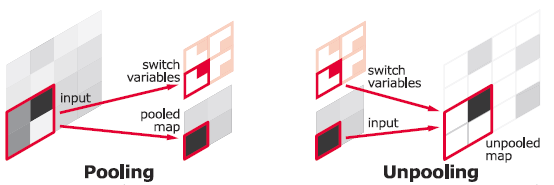
\includegraphics[scale=.6]{image/unpooling}
    \end{center}
    \caption{So sánh quá trình thực hiện max-pooling và un-pooling}
    \label{fig:unpooling}
    \end{figure}
\end{center}

\item \textbf{Deconvolution}: Lớp deconvolution hay còn có tên gọi khác là transposed-convolution, nhằm để tăng kích thước của giá trị đầu vào. Bằng cách thực hiện padding đủ lớn giá trị đầu vào, ta sẽ thực hiện được phép convolution lên giá trị mới này và và đạt được kết quả với kích thước lớn hơn.  


\begin{center}
    \begin{figure}[H]
    \begin{center}
     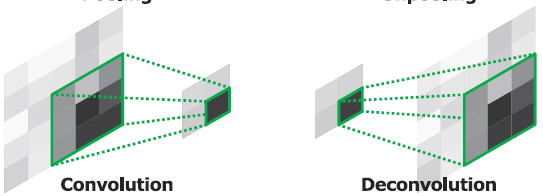
\includegraphics[scale=.6]{image/deconv}
    \end{center}
    \caption{So sánh quá trình thực hiện convolution và deconvolution}
    \label{fig:unpooling}
    \end{figure}
\end{center}


\end{enumerate}

% https://towardsdatascience.com/review-deconvnet-unpooling-layer-semantic-segmentation-55cf8a6e380e
 

\subsection{Biểu diễn ảnh RGB-D}
Ảnh RGBD là một tổ hợp của 3 kênh màu (đỏ,xanh lá cây và xanh dương) và thêm một kênh dữ liệu mới là độ sâu (depth data). Kênh màu có thể được biểu diễn bằng một ma trận của những số nguyên có 8 bit tương ứng từ 0 đến 255 nên nó biểu diễn được 256 màu tại mỗi điểm ảnh.\\

Độ sâu lại biểu diễn bằng một ma trận của những số nguyên có 16 bit nhưng thực tế nó chỉ dùng có 11 bit.
Kinect định giá trị của độ sâu trong khoảng từ 1 đến 10.000 giá trị đơn vị là milimet (1 đến 10.000mm).\\

Nhưng dữ liệu từ Kinect gặp phải một số vấn đề. Ảnh màu lẫn dữ liệu độ sâu đều có nhiễu. Bên cạnh đó cũng cần phải hiệu chỉnh lại những cái máy ảnh để tổng hợp ảnh màu và độ sâu sao cho chính xác.\\

Bức ảnh có thể có độ phân gải là 640x480 hoặc 1280x1024. Cả 2 độ phân giải này đều biểu diễn nhiễu về màu. Tương tự thì độ sâu cũng bị nhiễu và có những điểm ảnh lại không có được thông tin chiều sâu. Việc thiếu hụt này là do máy ảnh và bộ phát hồng ngoại nằm ở các vị trí khác nhau.\\

Viêc cần thiết là cần tiền xử lí lại dữ liệu bằng các phương pháp xử lí ảnh.


\section{ResNet}

Deep residual networks là một trong một những mô hình thể hiện sự đột phá trong lĩnh vực thị giác máy tính cũng như học sâu trong thời gian gần đây. Resnet có thể giúp huấn luyện những mô hình có số lượng layer rất lớn lên đến hàng trăm layer mà vẫn đạt được hiệu suất rất tốt. Với một lợi thế đáng kể như vậy, nó đã giúp cho nhiều ứng dụng thị giác máy tính có thể phân loại ảnh tốt hơn, điển hình là phát hiện đối tượng.\\

Tuy nhiên số layer càng lớn thì  mô hình càng dễ có xu hướng sẽ quá khớp (overfitting) với dữ liệu. Chúng ta có thể thấy xu hướng theo thời gian các mô hình ngày càng có số lượng layer tăng lên đáng kể, từ sau kiến trúc AlexNet thì các mô hình về sau đã có độ sâu tăng lên, AlexNet chỉ có 5 convolutional layers, VGG có 19 layers và GoogleNet có đến 22 layers. \\

Tăng số layer của một mô hình không đơn giản là xếp các layer chồng lên nhau, nếu chỉ xếp chồng lên đơn giản như vậy thì mô hình sẽ không hoạt động hiệu quả. Các mạng sâu rất khó để huấn luyện vì có thể sẽ gây ra hiện tượng triệt tiêu gradient trong quá trình backpropagation. Kết quả là khi mạng đi sâu thì hiệu suất dường như bị bão hòa và có xu hướng giảm xuống. Như theo hình \ref{fig:resnet_layer}, với số layer nhiều hơn, ta luôn nhận được lỗi trong quá trình huấn luyện cũng như lỗi trong quá trình đánh giá là lớn hơn.\\

\begin{center}
    \begin{figure}[H]
    \begin{center}
     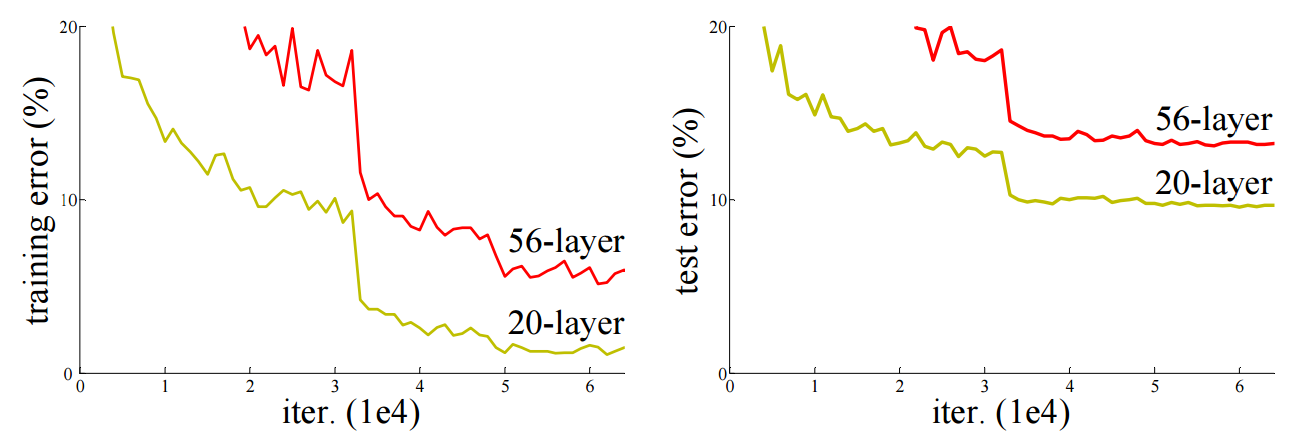
\includegraphics[scale=.25]{image/chapter3_resnet_compare}
    \end{center}
    \caption{Tăng số layer làm cho hiệu suất của mô hình giảm}
    \label{fig:resnet_layer}
    \end{figure}
\end{center}


Ý tưởng chính của Resnet là tạo ra một "identity shortcut connection" để có thể bỏ qua một hoặc nhiều layers, nếu như những layer đó đang bị triệt tiêu gradient, theo hình \ref{fig:resnet_block}.Các layers xếp chồng lên nhau, không làm cho hiệu suất của mạng bị suy giảm, do đã có các shortcut connection. Hiện nay, Resnet đã trở nên phổ biến, kiến trúc của nó được nghiên cứu rất nhiều và đã có khá nhiều những kiến trúc mới dựa trên Resnet.

\begin{center}
    \begin{figure}[H]
    \begin{center}
     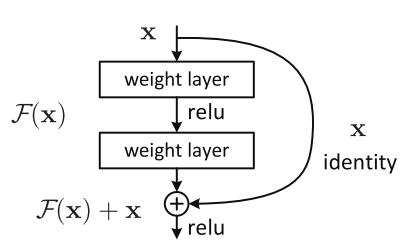
\includegraphics[scale=.5]{image/chapter3_resnet_block}
    \end{center}
    \caption{Một block của residual networks.}
    \label{fig:resnet_block}
    \end{figure}
\end{center}



 




 



\chapter{Hướng tiếp cận}

% \cite{laina2016deeper}
% abcde \cite{Ma2017SparseToDense} abcd \cite{ICF}


Ở chương này, nhóm sẽ trình bày chi tiết về mô hình ước lượng độ sâu được nhóm sử dụng cũng như các kĩ thuật liên quan.
% giới thiệu lại dùng mask-rcnn với cách tính khoảng cách gọn thôi
Ở giai đoạn ước lượng khoảng cách vật thể , nhóm sẽ sử dụng ảnh độ sâu có được ở mô hình trên và Mask RCNN\cite{He2017MaskR} thông qua các phương pháp mà nhóm đề xuất để mỗi vật thể được nhận diện trong ảnh RGB sẽ có khoảng cách tương ứng.

% Trong quá trình luận văn, nhóm sẽ tiếp cận vấn đề với 2 hướng
% \begin{itemize}
% \item Thực hiện bao đóng 3D vật thể dựa vào 2D proposals
% \item Từ bao đóng 2D, thực hiện matching model để phát hiện hình dáng của vật thể.
% \end{itemize}
\begin{comment} 
\section{Mô hình cơ bản}


Mô hình để dự đoán khoảng cách của vật thể sẽ dựa theo cấu trúc trên hình 5.1, được chia làm 3 nhiệm vụ: đầu tiên, ta sẽ dự đoán depth map của ảnh RGB dựa trên Fully Convolutional Residual Networks (FCRN), tiếp theo áp dụng Mask RCNN để tiến hình phát hiện, bao đóng, phân mảnh vật thể dựa trên ảnh RGB. Dựa vào kết quả của 2 mô hình trên, áp dụng các phương pháp khác nhau để có thể ước lượng được khoảng cách vật thể. 
\end{comment}

\section{Ước lượng ảnh độ sâu từ ảnh RGB}
Để dự đoán độ sâu từ một ảnh RGB, Laina et al. \cite{laina2016deeper} đã đề xuất fully convolutional residual network (FCRN), nó chỉ gồm một kiến trúc đơn nhất và được huấn luyện từ đầu đến cuối (end-to-end) mà không đòi hỏi các kĩ thuật hậu xử lí như các bước tinh chỉnh kết quả (refinement step). Sau đó, nhằm cải thiện độ tin cậy và chính xác của kết quả dự đoán độ sâu chỉ sử dụng một ảnh đơn. Ma et al. \cite{Ma2017SparseToDense} đã xây dựng mạng CNN có cấu trúc dựa trên FCRN, nhưng sử dụng một ảnh độ sâu thưa cùng với ảnh RGB để tái tạo lại một ảnh độ sâu có độ phân giải cao. Ảnh độ sâu thưa có thể được sinh ra từ các depth sensor có chi phí thấp, hoặc được tính toán bằng giải thuật Simultaneous Localization and Mapping (SLAM) như \cite{SLAM}. Đây chính là hướng tiếp cận của nhóm.\\

Ở mục 4.1 này, phần đầu nhóm sẽ trình bày kiến trúc mạng FCRN (fully covolutional neural network) của \cite{laina2016deeper}, nhằm ánh xạ một ảnh RGB sang ảnh độ sâu tương ứng. Ở phần sau nhóm sẽ nói về deep regression network của Ma et al.\cite{Ma2017SparseToDense} có đầu vào là ảnh RGB kết hợp với ảnh độ sâu thưa để hướng dẫn mạng dự đoán độ sâu tại mỗi điểm ảnh.  Ma et al.\cite{Ma2017SparseToDense} đã dùng kĩ thuật lấy mẫu độ sâu (depth sampling) từ ảnh độ sâu thực để tạo ra ảnh độ sâu thưa phục vụ cho quá trình huấn luyện mạng, kĩ thuật đó sẽ được nhóm làm rõ ở đây cũng như các kĩ thuật khác như data augmentation, hàm đo độ lỗi (loss function) được sử dụng trong quá trình tối ưu. 

%\subsection{Kiến trúc của mạng CNN}
%\subsection{Fully convolutional residual network}
\subsection{Dự đoán độ sâu từ một ảnh đơn với fully convolutional residual network}
Mạng fully convolutional residual network được đề xuất bởi Laina et al. \cite{laina2016deeper} lấy ý tưởng từ residual learning để dự đoán độ sâu. Như chúng ta đã biết ở chương trước, hầu hết các mạng CNN hiện nay gồm nhiều lớp mà mỗi lớp là một phép tính convolution hoặc pooling và khi một bức ảnh RGB được đưa vào mạng thì chuỗi phép tính này sẽ liên tục làm giảm độ phân giải của nó, điều này giúp cho các nơron càng thuộc về các lớp sau sẽ có vùng thụ cảm (receptive field) tương ứng càng lớn, dẫn đến lượng thông tin toàn cục mà nó nhận được sẽ lớn hơn các lớp trước. Ước lượng độ sâu là một bài toán hồi quy (regression) nhưng đầu ra mong muốn có độ phân giải cao, nên chúng ta sẽ cần các phép up-sampling để có được đầu ra lớn hơn. Eigen\cite{Eigen2014,Eigen2015} đã dùng lớp kết nối đầy đủ (fully-connected layers) để các nơron lớp này có vùng thụ cảm chứa toàn bộ bức ảnh làm cho nó có thể hiểu toàn cục khung cảnh, điều này là cần thiết vì nó có thể sử dụng hiệu quả hơn các đặc điểm như vị trí của đối tượng, hướng của căn phòng... so với việc chỉ hiểu được những phần cục bộ của bức ảnh để đưa ra những dự đoán khoảng cách tốt hơn. Nhưng việc dùng lớp kết nối đầy đủ để dự đoán độ sâu sẽ khiến mô hình tăng số lượng tham số , do đó độ phân giải của đầu ra sẽ không lớn như mong muốn.\\

Kiến trúc của Laina et al.\cite{laina2016deeper} đã tiến hành loại bỏ lớp kết nối đầy đủ, mỗi đầu vào được tùy chỉnh về size 304$\times$228, và đầu ra mong muốn là một nửa độ lớn của đầu vào, Laina et al.\cite{laina2016deeper} đã tiến hành khảo sát một số kiến trúc nổi tiếng như AlexNet\cite{Krizhevsky2012} và VGG-16\cite{Simonyan2014} bởi vì trọng số đã huấn luyện sẵn của các mô hình này giúp cho việc hội tụ tốt hơn và thấy rằng nếu bỏ đi lớp kết nối đầy đủ thì vùng thụ cảm của lớp convolutional cuối cùng của AlexNet là 151$\times$151, của VGG-16 là 276$\times$276 nó vẫn nhỏ hơn 304$\times$228, đây là độ lớn đầu vào của chúng ta. Do đó nó chưa đủ để hiểu thông tin toàn cục của bức ảnh, nhưng với sự ra đời của ResNet\cite{KHe2015} và ý tưởng residual learning, nó giúp tạo các mạng CNN cực sâu mà vẫn cho kết quả tốt hơn các mạng thông thường, đồng thời các mạng này có vùng thụ cảm lớn hơn. Với ResNet-50 nó có vùng thụ cảm là 483$\times$483 đủ lớn để tiếp nhận toàn bộ thông tin của đầu vào. Vậy với một bức ảnh 304$\times$228 thì lớp convolutional cuối cùng của  ResNet-50 sẽ cho ra 2048 feature map có độ phân giải 10$\times$8.  Nếu chúng ta dùng lớp kết nối đầy đủ để sinh ra đầu ra có độ phân giải là 160$\times$128 thì sẽ tốn mất 3.3 tỷ tham số và nó sẽ cần đến 12.6GB trong bộ nhớ, do đó sử dụng phương pháp này là không thể so  với phần cứng hiện tại. Do đó Laina et al.\cite{laina2016deeper} đã dùng một vài phép residual up-covolution thay cho lớp kết nối đầy đủ để đạt được đầu ra có độ lớn 160$\times$128, điều này đã giúp cho mạng fully convolutional chứa ít tham số hơn cũng như cải thiện được độ chính xác của việc dự đoán độ sâu.\\

Tóm lại kiến trúc đề xuất của Laina et al.\cite{laina2016deeper} gồm 2 phần. Phần đầu của mạng là dựa trên ResNet-50 \cite{KHe2015}, nó đã bị bỏ lớp average pooling và lớp kết nối đầy đủ cuối cùng. Phần sau của kiến trúc sẽ hướng dẫn mạng học cách tăng độ phân giải của feature map bằng bốn lớp upsampling và cuối cùng là dùng phép bilinear interpolation để có độ phân giải bằng với đầu ra ban đầu.
 \begin{center}
         \begin{figure}[H]
         \begin{center}
           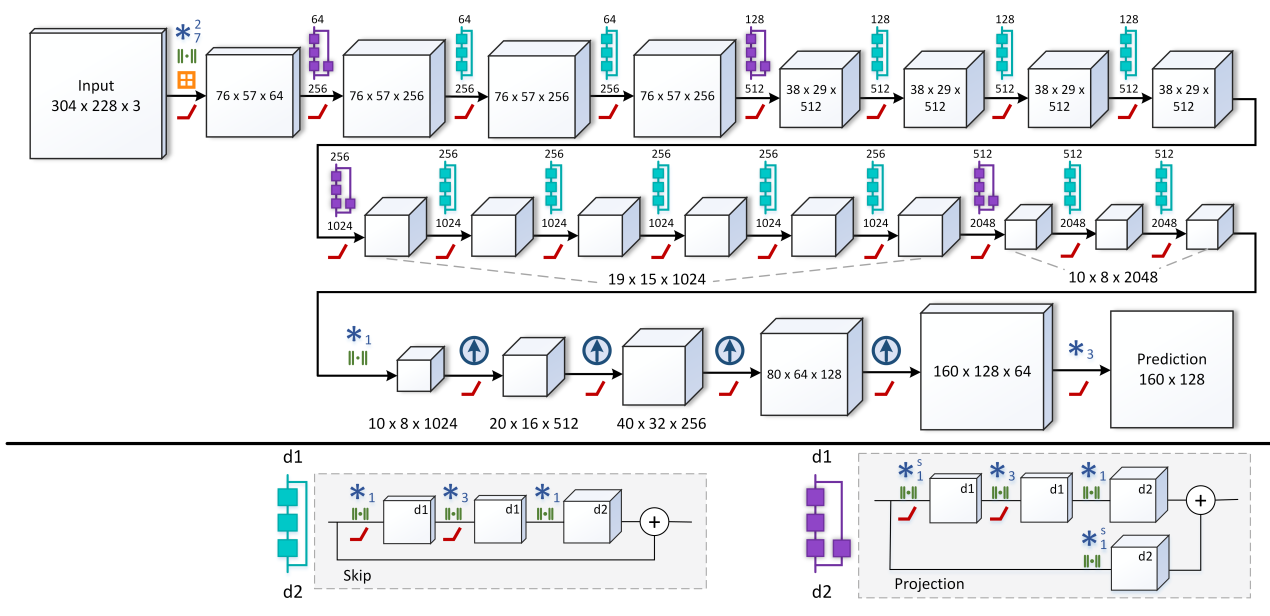
\includegraphics[scale=0.35]{image/LainaNet}
          \end{center}
          \caption{Kiến trúc của FCRN. Mỗi khối là một feature map với số chiều là $\#height\times width\times channel$, phần đầu là ResNet-50\cite{KHe2015}, output của nó là khối 10$\times$8$\times$2048 cuối cùng, sau đó là 1 lớp 1$\times$1 convolution và 4 phép upsampling, cuối cùng là 1 phép 3$\times$3 convolution để sinh ra output với độ phân giải một nửa so với input }
          \label{ref_sigmoid}
          \end{figure}
 \end{center}
% Chúng ta sẽ thiết lập để input có size là 304 x 228 và một khía cạnh quan trọng ảnh hưởng đến chất lượng của kết quả dự đoán độ sâu đó chính là vùng thụ cảm.Cho nên các neuron này nó nhận diện được các đặc trưng rất phức tạp của bức ảnh, điều này thể hiện rõ qua các kiến trúc nổi tiếng như AlexNet\cite{Krizhevsky2012} và VGGNet\cite{Simonyan2014}. Vùng thụ cảm ở lớp convolutional cuối của AlexNet và của VGG tương ứng là 151 x 151 pixels  và 276 x 276, kết quả là VGGNet cho lỗi nhỏ hơn AlexNet trong bài toán phân loại ảnh. Nhưng ở đây 276 x 276 vẫn nhỏ hơn 304 x 228 chưa đủ để  , may mắn thay ResNet\cite{K.He2015} với 
%Mô hình của \cite{Ma2017SparseToDense} khác với \cite{laina2016deeper} ở chỗ là chúng nhận đầu vào có depth channel không nhất thiết là 3 như \cite{laina2016deeper}. Để một mạng CNN ánh xạ một bức ảnh RGB sang một depth map, thì nó phải khả năng tìm ra được được mối liên hệ giữa giá trị của các kênh (channel) R, G, B tại mỗi điểm ảnh và giữa các điểm ảnh với nhau, đối với khoảng cách tương ứng của chúng. Như ta đã biết các mạng CNN như AlexNet\cite{Krizhevsky2012}, VGGNet\cite{Simonyan2014} và ResNet\cite{K.He2015} là những mô hình chiến thắng ở cuộc thi ILSVRC qua các năm 2012, 2014, 2015 và chúng đã giải quyết rất tốt bài toán phân loại ảnh (thậm chí tỉ lệ lỗi ResNet đã vượt qua con người). Tại đó chúng ánh xạ mỗi bức ảnh thành nhãn tương ứng, 
%như \cite{Zeiler2014} thì các mạng CNN trên gồm nhiều lớp ở mỗi lớp gồm nhiều neuron, mỗi neuron sẽ nhận diện những đặc trưng riêng của bức ảnh và một đặc tính khá thú vị là các neuron càng thuộc về các lớp sau đặc trưng mà nó nhận diện được càng phức tạp. Đây là điều chúng ta muốn, các đặc trưng riêng của mỗi bức ảnh nhưng thay vì gán nhãn cho nó, chúng ta đem những đặc trưng này ánh xạ sang độ sâu..\\
%Tóm lại mạng CNN mà nhóm dùng ước lượng độ sâu sẽ có bộ encoder nhằm rút trích đặc trưng của ảnh RGB sau đó những đặc trưng này được đưa vào bộ decoder gồm 1 vài phép up-sampling để được output có độ phân giải mong muốn. 
\begin{comment}
\subsubsection{Mô hình encoder}
 như đã trình bày ở chương 3. Cho nên ác .
%Nên các neuron thuộc lớp trước lớp fully connected cuối cùng của các mạng AlexNet, VGGNet, ResNet... nắm giữ những feature quan trọng giúp phân loại bức ảnh. Do đó người ta thường bỏ đi lớp cuối của các mạng trên và đem phần còn lại sử dụng như một bộ trích xuất đặc trưng để giải quyết những bài toán khác.\\
 Bài toán ước lượng độ sâu thực chất là bài toán hồi quy (regresion) mà tại đó output mà chúng ta mong muốn là bức ảnh độ sâu (depth map) có độ phân giải cao. Để có được output lớn hơn chúng ta sẽ dùng một vài phép up-sampling để qua các phép tính này độ phân giải sẽ được nâng lên từ từ.
Tóm lại mô hình encoder của nhóm sẽ là một mạng CNN phổ biến dùng để trích xuất đặc trưng của bức ảnh, sau đó kết nôi với bộ decoder là một vài phép up-sampling sao cho độ phân giải cúa output bằng với input.

Để trích xuất đặc trưng của nah nhóm chọn resnet:\\
Ưu điểm của resnet: resnet là một mạng CNN rất sâu đó nhưng khi lan truyền ngược đạo hàm không bị triệt tiêu các lớp đầu. Điều đó khiến nó dễ hội tụ nhưng còn một lợi thế khác là nó có vùng thụ cảm (receptive field) lớn,ví dụ: resnet50 là 483 x 483. Đủ lớn để lấy được thông tin của những bức ảnh đầu váo lớn hơn.
\subsubsection{Mô hình decoder}
\end{comment}
Từ những feature đã lấy được từ ResNet, nhóm sẽ tiến hành up-scaling những đặc điểm đã được trích xuất để tiến sinh ảnh độ sâu. Với quá trình up-scaling, nhóm tiến hành thử nghiệm với những cấu trúc khác nhau, gồm nhiều block liên tiếp nhau. Dưới đây sẽ mô tả cấu trúc của từng loại block.

\begin{itemize}
	\item Deconvolution 2: Thực hiện deconvolution với kernel size là 2$\times$2 để up-scaling feature map lên kích thước mong muốn đạt được.
	\item Deconvolution 3: Tương tự như deconvolution 2 nhưng được thực hiện với kernel size là 3$\times$3. 
	\item Up-convolution: Đầu tiên, ta thực hiện phép Unpooling 2$\times$2 trên feature map và nhận được kết quả là một feature map có kích cỡ lớn gấp đôi. Tiếp theo, thực hiện convolution với kernel size 5$\times$5, padding để giữ nguyên chiều cao, chiều rộng của input và số filter sẽ bằng một nửa số channel của đầu vào. Sau cùng thực hiện ReLU trên kết quả.  Hình bên dưới mô tả cấu trúc của một up-convolution block. 
      \begin{center}
         \begin{figure}[H]
         \begin{center}
           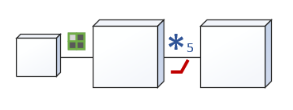
\includegraphics[scale=0.6]{image/up_conv}
          \end{center}
          \caption{Up-convolution block}
          \label{ref_sigmoid}
          \end{figure}
      \end{center}
    
    \item Up-projection: dựa trên cơ sở của up-convolution, đồng thời, up-projection cũng kế thừa ý tưởng skip connection của Resnet. Một nhánh sẽ kế thừa từ up-convolution và được gắn thêm một lớp convolution kernel size là 3$\times$3. Nhánh còn lại sẽ chỉ thực hiện convolution với kernel size 5$\times$5, trực tiếp từ kết quả của Unpooling. Với việc cộng lại kết quả từ cả 2 nhánh và thực hiện ReLU, ta có kết quả sau cùng của một uprojection block. Hình bên dưới mô tả khá rõ về cấu trúc của 1 uprojection block.
    
     \begin{center}
         \begin{figure}[H]
         \begin{center}
           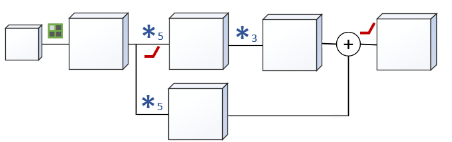
\includegraphics[scale=0.7]{image/up_projection}
          \end{center}
          \caption{Up-projection block}
          \label{ref_sigmoid}
          \end{figure}
      \end{center}
 \end{itemize}

\subsection{Dự đoán độ sâu dựa vào mẫu độ sâu thưa và một ảnh đơn với deep regression network}
Như những gì đã trình bày ở trên, nhận thấy việc chỉ dựa vào thông tin màu sắc như giá trị R, G, B để đưa ra dự đoán về độ sâu thì tính chính xác và độ tin cậy của phương pháp trên vẫn xa so với thực tế mặc dù rất nhiều nỗ lực nghiên cứu trong một thập kỉ qua dành cho phương pháp dự đoán độ sâu từ một ảnh đơn bao gồm cả những tiến bộ gần đây của kĩ thuật học sâu, cho nên ngoài việc sử dụng ảnh RGB, Ma et al.\cite{Ma2017SparseToDense} đã xem xét sử dụng thêm ảnh độ sâu thưa, đây là một bức ảnh độ sâu nhưng chỉ có một ít điểm ảnh có giá trị, còn những điểm ảnh còn lại giá trị của nó chỉ là 0. Tuy chỉ có một vài điểm có giá trị nhưng những thông tin bổ sung này đóng vai trò cực kì quan trọng giúp cho mạng CNN cải thiện đáng kể kết quả dự đoán của mình.
\subsubsection{Kiến trúc CNN của mạng deep regression network}
Kiến trúc mạng CNN của Ma et al.\cite{Ma2017SparseToDense} giống như mạng FCRN của Laina et al.\cite{laina2016deeper}, nhưng khác với FCRN thì deep regression network (DRN) của Ma còn dùng thêm ảnh độ sâu thưa, nên đầu vào của DRN là một ảnh RGB-D có channel là 4 tương ứng với 4 giá trị R, G, B và D là thông tin độ sâu tại điểm ảnh đó. Chi tiết kiến trúc được thể hiện ở hình bên dưới.
\begin{center}
         \begin{figure}[H]
         \begin{center}
           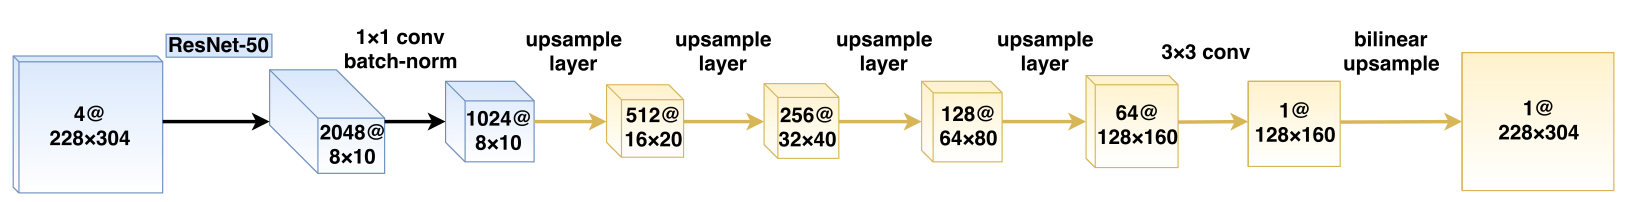
\includegraphics[scale=0.28]{image/Manet}
          \end{center}
          \caption{Kiến trúc CNN cho tập dữ liệu NYUv2 dựa trên Laina\cite{laina2016deeper}. Các khối chính là feature maps với chiều được biểu diễn bằng $\#channel@height\times width$. Các khối màu xanh là các lớp encoding bao gồm ResNet\cite{KHe2015} và 1$\times$1 convolution. Các lớp màu vàng gồm 4 lớp upsampling, một lớp 3$\times$3 convolution và một phép bilinear upsample để nâng độ phân giải về ban đầu}
          \label{ref_sigmoid}
          \end{figure}
 \end{center}

\subsubsection{Depth sampling}
Ở đây nhóm sẽ nói về chiến lược lấy mẫu để sinh ra ảnh độ sâu thưa từ ảnh độ sâu thực tế mà ta có (ground truth).\\

Trong suốt quá trình huấn luyện, ảnh độ sâu thưa $D$ sẽ được lấy mẫu ngẫu nhiên từ ảnh độ sâu thực tế $D^{*}$. Cụ thể, với mỗi một số mẫu độ sâu $m$ (cố định trong suốt quá trình huấn luyện), chúng ta tính xác suất Bernoulli $p = \frac{m}{n}$, mà $n$ là tổng số điểm ảnh hợp lệ của $D^{*}$. Điểm ảnh hợp lệ ở đây là những điểm ảnh có giá trị độ sâu không vượt quá một giá trị cho trước (giá trị này được thiết lấp cố định lúc huấn luyện). Tiếp theo, với mỗi điểm ảnh $\left (i, j \right)$,
\begin{center}
$\textit{D}\left ( i,j \right ) = \begin{cases}
 & D^{*}\left (i,j \right ),\hspace{.5cm} \text{với xác suất }  p\\ 
 & 0, \hspace{1.7cm} \text{trường hợp khác} 
\end{cases}$

\end{center}

Với chiến lược lấy mẫu này thì số lượng điểm ảnh có giá trị độ sâu khác 0 sẽ biến đổi đối với mỗi mẫu huấn luyện (training sample) xung quanh giá trị trung bình $m$. Mục đích của nó còn giúp tăng lượng dữ liệu huấn luyện giống như kĩ thuật data augmentation được trình bày sau đây.

\subsubsection{Data augmentation}

Để tăng lượng dữ liệu cho tập huấn luyện thì Ma et al.\cite{Ma2017SparseToDense} đã dùng nhiều phương pháp chuyển đối dữ liệu gốc một cách ngẫu nhiên trong quá trình huấn luyện đối với mỗi mẫu (trainning sample) tham gia.\\
Các phương pháp dưới đây áp dụng cho cả ảnh màu và ảnh độ sâu
\begin{itemize}
\item Rotation: quay một góc ngẫu nhiên $r$ $\in$ [5, -5]
\item Scale:  Nâng độ phân giải lên một hệ số ngẫu nhiên $s$ $\in$ [1, 1.5]
\item Centercrop: Chúng ta sẽ tiến hành crop trung tâm từ bức ảnh để độ phân giải của mỗi input là như nhau.
\item Flips: Ở đây ta sẽ đổi chiều bức ảnh theo chiều ngang với xác suất là 0.5
\end{itemize}
Riêng đối với ảnh màu ta còn chỉnh độ sáng, tương phản bằng các hệ số $k_{i} \in $ [0.6, 1.4] và chuẩn hóa bằng cách chia tất cả giá trị R, G, B cho 255.

\subsubsection{Hàm đo độ lỗi}
Với bài toán hồi quy thì hàm đo độ lỗi (loss function) chuẩn dùng trong qúa trình tối ưu là hàm trung bình bình phương lỗi (mean squared error) giữa giá trị thực tế y và giá trị dự đoán $y^{*}$: $L_{2}\left(y^{*} - y\right)$ = $\left \|y^{*} - y \right \|^{2}$. Hàm $L_{2}$ có ý nghĩa như sau, nếu giá trị lỗi càng lớn thì các thành phần gây ra lỗi sẽ bị phạt thật nặng để giảm lỗi. Nhưng với bài toán này Ma et al.\cite{Ma2017SparseToDense} đã cho thấy kết quả từ việc sử dụng $L_{2}$ không được tốt.\\
Một lựa chọn phổ biến khác là hàm lỗi berHu được Laina et al.\cite{laina2016deeper} sử dung:
\begin{center}
$\textit{B}\left ( e \right ) = \begin{cases}
 & \left | e \right |,\hspace{.8cm} \text{nếu}  \left | e \right | \leq  c\\ 
 & \frac{e^{2} + c^{2}}{2c}, \hspace{.4cm} \text{nếu} \left | e \right | >  c
\end{cases}$

\end{center}
Với $e = y_i^{*} - y_i$, và tại mỗi bước gradient descent, ta có $c = \frac{1}{5}\max_i\left(\left |y_i^{*} - y_i \right | \right)$, ta xét $i$ là toàn bộ điểm ảnh trên mỗi ảnh tại bó hiện tại (current batch). Ta có thể thấy được hàm berHu sẽ trở thành hàm trung bình trị tuyệt đối lỗi $L_1$ (mean absolute error) nếu như $ e \leq c$, và nó sẽ xấp xỉ $L_2$ khi lỗi vượt qua ngưỡng c, nhưng hàm này vẫn có đạo hàm tại c. Về mặt trực giác ta thấy khi một điểm ảnh có $e$ nhỏ thì berHu là hàm $L_1$ và thông thường đạo hàm theo $L_1$ lớn hơn $L_2$ và ngược lại khi $e$ lớn thì berHu xấp xỉ hàm $L_2$ và đạo hàm theo $L_2$ lại nhỏ hơn $L_1$, điều này giúp nó hội tụ tốt hơn. Nhưng nó cũng đòi hỏi chi phí tính toán lớn hơn để tìm ra hằng số c.\\

Trong những thí nghiệm của mình Ma at el. \cite{Ma2017SparseToDense} đã cho thấy $L_1$ đạt kết quả tốt hơn một chút so với berHu, nên nhóm đã chon $L_1$ làm lựa chọn mặc định vì sự đơn giản cũng như chi phí tính toán thấp hơn so với berHu.



\section{Ước lượng khoảng cách vật thể}

Như nhóm đã đề cập từ trước, để có thể ước lượng được khoảng cách vật thể từ một bức ảnh, thì nhiệm vụ đầu tiên, đó chính là phát hiện đó là vật thể gì, vật thể đó ở vị trí nào trong ảnh, đồng thời phải bao đóng và phân đoạn đối tượng đó. Đây là một bài toán kinh điển trong mảng thị giác máy tính và gây khó khăn cho nhiều nhà nghiên cứu. Là con người, chúng ta có thể dễ dàng nhìn, và biết được chúng ta đang nhìn gì, đồng thời có thể ước lượng được khoảng cách những vật đó cách chúng ta bao xa dựa trên kinh nghiệm. Nhưng với một cỗ máy, để thực hiện được nhiệm vụ trên đòi hỏi nhiều công nghệ, cũng như kết hợp nhiều kết quả nghiên cứu. Hiện nay, đã có nhiều mô hình cho kết quả rất tốt trong việc phát hiện, bao đóng và phân đoạn vật thể: SSD, Mask RCNN ... 

% Nói cách khác, chúng ta sẽ chỉ tập trung vào những bao đóng, phân đoạn chứa vật thể để có thể tối ưu hóa độ chính xác của việc ước lượng khoảng cách, giảm việc bị ảnh hưởng của những thông tin ko liên quan đến vật thể như môi trường...

\subsection{Phát hiện, bao đóng và phân đoạn vật thể}

Trong những mô hình thực hiện nhiệm vụ phát hiện, bao đóng và phân đoạn vật thể mà nhóm tìm hiểu, thì Mask RCNN \cite{He2017MaskR} là một trong những mô hình tốt nhất và cho kết quả rất tốt cả về phát hiện, bao đóng vật thể lẫn phân đoạn. Do vậy, nhóm quyết định sử dụng Mask RCNN  để kết hợp với ảnh độ sâu, là kết quả từ mô hình FCRN, nhằm giải quyết mục tiêu xác định khoảng cách vật thể.\\

Từ một ảnh RGB ban đầu, Mask RCNN sẽ cho ra kết quả là bao đóng, phân đoạn từng loại vật thể có trong ảnh. Nói cách khác, dựa trên kết quả của Mask RCNN, chúng ta sẽ chỉ tập trung vào những bao đóng, phân đoạn chứa vật thể nhằm giảm thiểu việc ảnh hưởng của những thông tin không cần thiết như những vật thể không liên quan, môi trường, ...

\subsection{Ước lượng khoảng cách vật thể}

% Với kết quả thu được từ 2 mô hình Mask RCNN và FCRN, chúng ta hiện đã có được bao đóng, phân đoạn của vật thể và ảnh độ sâu của ảnh RGB. 

Hiện nay, chúng ta có thể thấy được sự đa dạng của vật thể, không chỉ về mặt số lượng mà còn về hình dáng, kích thước. Do vậy, sẽ không có một khái niệm hoàn toàn chính xác của việc đo khoảng cách vật thể. Tùy mỗi trường hợp, mỗi mục tiêu để có thể đề xuất các cách đo khác nhau. Chẳng hạn, với những vật thể nhỏ như chai nước, điện thoại, thì khoảng cách sẽ thường được ước lượng bằng khoảng từ camera đến tâm của vật thể. Mặt khác, đối với vật thể có mô hình phức tạp hơn, như cái ghế, cái bàn, thì chúng ta cần những phương thức khác nhau để có thể ước lượng được khoảng cách.\\

Ngoài ra, nếu chỉ dựa vào kết quả bao đóng vật thể, thì những thông tin của môi trường còn nằm trong bao đóng vẫn sẽ ảnh hưởng không nhỏ đến kết quả của việc ước lượng khoảng cách. Do vậy, việc kết hợp với kết quả phân đoạn vật thể của Mask RCNN là cần thiết. \\

Dựa vào kết quả của FCRN, nhóm đã có ảnh độ sâu tương ứng của ảnh màu. Mỗi vị trí trên ảnh màu sẽ có một ước lượng độ sâu tương ứng được chứa trong ảnh độ sâu. Bằng việc kết hợp các kết quả bao đóng, phân đoạn vật thể và ảnh độ sâu, nhóm đề xuất những phương án để có thể ước lượng được khoảng cách của vật thể và đánh giá, so sánh kết quả của những phương án đã đề xuất. 

\begin{itemize}

% \item \textbf{Phương án 1}: Ước lượng khoảng cách bằng các điểm nằm trong bao đóng của vật thể. Ở đây, nhóm sẽ lấy kết quả ước lượng độ sâu từ ảnh độ sâu của tất cả những điểm nằm trong bao đóng vật thể. Kết quả của phương án này nhằm đánh giá sự ảnh hưởng của thông tin môi trường nằm trong bao đóng ảnh hưởng như thế nào đối việc ước lượng khoảng cách khi so sánh với các phương án khác.

\item \textbf{Phương án 1}: Ước lượng khoảng cách bằng lấy mẫu những điểm  xung quanh tâm bao đóng của vật thể, theo phân bố Gaussian. Với cảm quan của con người, chúng ta thường ước lượng khoảng cách dựa trên tâm của vật thể. Việc lấy những điểm xung quanh tâm bao đóng theo phân bố Gaussian cũng dựa trên kinh nghiệm này. Bên cạnh đó, với việc giảm số điểm chúng ta lấy để ước lượng khoảng cách, thì các giá trị gây nhiễu từ những điểm nằm trong bao đóng nhưng không thuộc vật thể sẽ được giảm.

\item \textbf{Phương án 2}: Ước lượng khoảng cách dựa trên kết quả phân đoạn của Mask RCNN. Ở đây, nhóm sẽ lấy tất cả những điểm  mà Mask RCNN cho là thuộc về vật thể để ước lượng khoảng cách. Theo hướng tiếp cận này, việc gây nhiễu của những điểm không thuộc vật thể sẽ được loại bỏ dựa vào kết quả phân đoạn.

\item \textbf{Phương án 3}: Ước lượng khoảng cách bằng cách lấy mẫu những điểm xung quanh tâm bao đóng của vật thể theo phân phối Gaussian, trong đó những điểm này phải được Mask RCNN cho là thuộc về vật thể. Phương án này dựa trên việc kết hợp kết quả phân đoạn của Mask RCNN và việc ước lượng khoảng cách dựa trên tâm vật thể.  

\end{itemize}





\chapter{Hiện thực mô hình}

\section{Công cụ}

Trong quá trình hiện thực, nhóm cũng sử dụng các công cụ có sẵn để giúp ít cho việc huấn luyện mô hình, tăng hiệu suất lập trình. Nhóm sử dụng chủ yếu hai framework là Keras và Pytorch. Với nhiệm vụ phát hiện, bao đóng vật thể và segmentation, thì nhóm đã sử dụng mô hình có sẵn được viết bằng Keras của tác giả khác để sử dụng . Framework thứ hai mà nhóm sử dụng là Pytorch, ưu điểm của nó là có thể chạy linh động (dynamic), được nhóm dùng để hiện thực Fully Convolution Residuals Networks, cũng như kết hợp cả 2 mô hình trên nhằm mục tiêu dự đoán khoảng cách vật thể.

\subsection{Pytorch}
% mi viết cái ni nghe vũ
Pytorch là một framework được phát triển bởi Facebook. Pytorch sử dụng dynamic graph, đây là một tính năng khá có sức hút đối với các nhà nghiên cứu và kĩ sư thường làm việc với dữ liệu về time-series và xử lý ngôn ngữ tự nhiên. Pytorch được tạo ra để vận dụng các thư viện trên Torch, đưa các thư viện này lên ngôn ngữ Python để sử dụng giúp mở rộng sự phổ biến, vì Torch được sử dụng trên ngôn ngữ Lua nên ít được phổ biến. Pytorch được tích hợp với Python khá sâu và nó theo dạng hướng đối tượng. Pytorch cũng cho phép mở rộng các chức năng một cách dễ dàng bằng cách khai báo những lớp kế thừa Pytorch. Giả sử, khi muốn tạo ra một lớp neural network bằng cách chỉnh sửa từ một lớp neural network có sẵn thì có thể kế
thừa từ nn.Module. Pytorch cung cấp 3 mức ở dạng trừ tượng để giúp mọi thứ dễ dàng sử dụng. Tensor trong Pytorch bắt buộc ở dạng nd-array, nó cũng giống với numpy nhưng lại có thể chạy được trên GPU. Biến (variable) là node trong sơ đồ tính toán computational graph) nó rất giống với tensor, variable, placeholder trong Tensorflow. Module là neural network layer, có thể lưu trữ các trọng số (weights). Pytorch ra đời muộn nhưng lại rất phổ biến trong cộng đồng nghiên cứu.
\subsection{Keras}
Keras là framework về học sâu,là dạng API, được viết bằng Python, và có thể chạy với các backend: Tensorflow, Theano, CNTK. Keras là một framework dễ tiếp cận, sử dụng, cho phép người dùng lập trình một cách nhanh chóng, dễ đọc, không rườm rà. Đặc biệt, ta có thể dễ dàng mở rộng, thêm các components mới vào mô hình đã có. Mặt khác, Keras cũng hỗ trợ đầy đủ các lớp trong mạng CNN và mạng RNN, có thể chạy được trên đồng thời CPU, GPU.
\begin{comment}
\section{Công việc cần chuẩn bị cho quá trình huấn luyện mô hình}

\subsection{Xử lý dữ liệu}

Sau khi tìm hiểu các tập dữ liệu về ảnh RGB-D, nhóm quyết định chọn bộ dữ liệu NYUV2. Đây là bộ dữ liệu được thu thập bằng máy Microsoff Kinect, với rất nhiều ngữ cảnh trong nhà khác nhau. Tập dữ liệu gồm 2 phần chính, đó là tập dữ liệu thô lên đến 407204 ảnh, và tập dữ liệu đã được đánh nhãn với 1449 ảnh. Với mục tiêu chính nhằm mục đích hiểu, có thể phân tích và đánh giá các mô hình dự đoán ảnh độ sâu, đồng thời với những khó khăn về phần cứng, nhóm quyết định chủ yếu sẽ tiến hành thí nghiệm trên tập dữ liệu nhỏ đã đánh nhãn với 1449 ảnh. 

\section{Quá trình huấn luyện mạng FCRN}
\subsection{Tài nguyên sử dụng}
Để tăng tốc quá trình huấn luyện nhóm đã sử dụng một GPU NVIDIA GTX 1080 có dung lượng ram là 8GB. Việc dùng GPU thay cho CPU nhằm tận dụng được khả năng tính toán song song vượt trội mà GPU mang lại.
\subsection{Kế hoạch huấn luyện}
\end{comment}
\section{Hiện thực mô hình ước lượng độ sâu và tiến hành thí nghiệm}
\subsection{Xử lý dữ liệu}

%Sau khi tìm hiểu các tập dữ liệu về ảnh RGB-D, nhóm quyết định chọn bộ dữ liệu NYUV2 \cite{silberman2012indoor}. Đây là bộ dữ liệu được thu thập bằng máy Microsoff Kinect, với rất nhiều ngữ cảnh trong nhà khác nhau. Tập dữ liệu gồm 2 phần chính, đó là tập dữ liệu thô lên đến 407204 ảnh, và tập dữ liệu đã được đánh nhãn với 1449 ảnh. Với mục tiêu chính nhằm mục đích hiểu, có thể phân tích và đánh giá các mô hình dự đoán ảnh độ sâu, đồng thời với những khó khăn về phần cứng, nhóm quyết định chủ yếu sẽ tiến hành thí nghiệm trên tập dữ liệu nhỏ đã đánh nhãn với 1449 ảnh. 
Sau khi tìm hiểu các tập dữ liệu về ảnh RGB-D, nhóm quyết định chọn bộ dữ liệu NYU-Depth V2 \cite{silberman2012indoor}. Đây là bộ dữ liệu được thu thập bằng máy Microsoff Kinect, với rất nhiều khung cảnh trong nhà khác nhau. Nó có đặc điểm:
\begin{itemize}
\item Tập dữ liệu được đánh nhãn có 1449 cặp ảnh gồm ảnh RGB và ảnh độ sâu tương ứng.
\item Có 464 khung cảnh khác nhau
\item Tập dữ liệu thô có số lượng ảnh lên đến 407204 ảnh.
\end{itemize}
Với mục tiêu chính nhằm mục đích hiểu, có thể phân tích và đánh giá các mô hình dự đoán ảnh độ sâu, đồng thời với những khó khăn về phần cứng, nhóm quyết định chủ yếu sẽ tiến hành thí nghiệm trên tập dữ liệu đánh nhãn.
\subsubsection{Tập dữ liệu đánh nhãn}
Tập dữ liệu này là tập con của tập dữ liệu thô. Nó bao gồm các cặp ảnh RGB và ảnh độ sâu cùng với một tập nhãn dày tương ứng, thêm vào đó ảnh độ sâu này đã được tiền xử lí để những giá trị độ sâu bị thiếu được điền đầy đủ bằng cách sử dụng  colorization scheme of Levin et al. \cite{nyu}
\begin{center}
         \begin{figure}[H]
         \begin{center}
           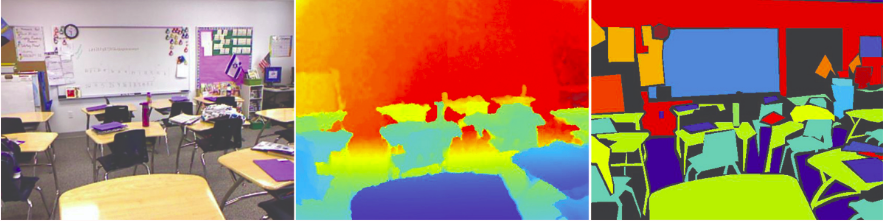
\includegraphics[scale=0.5]{image/nyu}
          \end{center}
          \caption{ảnh RGB (trái), ảnh độ sâu đã được xử lí (giữa), một tập các nhãn (phải) cho bức ảnh }
          \label{ref_sigmoid}
          \end{figure}
 \end{center}
 
 Tập dữ liệu này đã được chia làm 2 phần, gồm có 795 ảnh cho quá trình huấn luyện và 654 ảnh cho quá trình kiểm tra, nhận thấy tập kiểm tra chiếm 45\% của toàn bộ tập dữ liệu, nên nhóm tiến hành chia lại tập dữ liệu sao cho quá trình huấn luyện chiếm khoảng 80\% tập dữ liệu, thành 3 phần bằng cách lấy ngẫu nhiên 205 ảnh của tập kiểm tra bổ sung và tập huấn luyện và lấy thêm 159 ảnh cũng từ tập kiểm tra để tạo một tập xác thưc (validation set). Cuối cùng nhóm có tập huấn luyện có 1000 ảnh, tập xác thực có 159 ảnh và tập kiểm tra có 290 ảnh. Các ảnh này ban đầu có kích thước là 640$\times$480 sau đó được giảm xuống còn một nửa và tiến hành lấy trung tâm (center crop) để cuối cùng có kích thước là 304$\times$228.
\subsection{Thí nghiệm}
Mô hình deep regression network được hiên thực trên PyTorch,
\subsubsection{Tài nguyên sử dụng}
Nhóm đã sử dụng một GPU NVIDIA GTX 1080 có dung lượng RAM là 8GB nhằm tận dụng khả năng tính toán song song mà GPU hỗ trợ để tăng tốc quá trình huấn luyện.
\subsubsection{Chiến lược huấn luyện}
Trong quá trình huấn luyện nếu chỉ sử dụng ảnh RGB làm đầu vào thì phần trọng số của ResNet ở những lớp encoding sẽ được khởi tạo bằng trọng số ResNet đã được huấn luyện trên tập dữ liệu ImageNet \cite{Imagenet}. Còn đối với việc huấn luyện sử dụng đầu vào là ảnh RGB và ảnh độ sâu thưa thì đầu vào sẽ có 4 chiều RGB-D, nên lớp đầu tiên sẽ có channel vào (inchannels) là 4 do đó trọng số sẽ được khởi tạo theo phân phối Gaussian như sau:
\begin{itemize}
\item Nếu lớp cần được khởi tạo là một lớp convolution thì  $ w \sim  N( \mu = 0,\sigma ^{2} = \frac{2}{n} )$ với $n$ là tích của chiều dài, chiều rộng của kernel và số kernel của lớp đó.
\item Nếu lớp cần được khởi tạo là một lớp deconvolution thì $ w \sim  N( \mu = 0,\sigma ^{2} = \frac{2}{n} )$ $n$ là tích của chiều dài, chiều rộng của kernel và số channel của feature map của lớp trước của lớp đó.
\end{itemize}

Cách trên còn được áp dụng để khởi tạo các lớp deconvolution hoặc các lớp convolution của khối Up-projection thuộc các lớp decoding của mạng. Sau đây là các  siêu tham số (hyperparameter) mà nhóm đã thực hiện trong qúa trình huấn luyện. Số lượng mỗi bó (batchsize) trong quá trình huấn luyện là 8, tối ưu bằng phương pháp SGD với momentum\cite{momentum} với hệ số momentum là 0.9, hệ số học (leaning rate) ban đầu là 0.01 cứ sau 10 epoch sẽ giảm 10 lần. Hệ số weight decay là $10^{-4}$ được áp dụng để chính quy hóa (regularization).
Trong quá trình huấn luyện nhóm sẽ tiến hành đánh giá chất lượng mô hình sau mỗi epoch trên tập xác thực (valadation set) thông qua các độ đo được trình bày ở chương 6. Kết thúc quá trình huấn luyện thì mô hình cho kết quả tốt nhất trên tập xác thực sẽ được giữ lại.


\section{Quá trình ước lượng khoảng cách của vật thể}

Sau khi có được mô hình FCRN, nhóm sẽ tiến hành kết hợp kết quả của mô hình này với Mask RCNN nhằm ước lượng khoảng cách vật thể. Theo như nhóm đã trình bày trong hướng tiếp cận, việc ước lượng sẽ được thực hiện theo 4 phương án:
% một là dựa trên kết quả phát hiện bao đóng vật thể, tiến hành lấy các điểm mẫu bằng các phân bố ngẫu nhiên những điểm xung quanh tâm bao đóng của vật thể và kết quả depth map từ FCRN để ước lượng. Hướng thứ hai là sử dụng kết quả segmentation, lấy toàn bộ những pixel thuộc vật thể và kết quả depth map từ FCRN để ước lượng.
\subsection{Ước lượng khoảng cách bằng các điểm nằm trong bao đóng của vật thể}
Theo hướng này, chúng ta sẽ lấy tất cả những điểm nằm trong bao đóng của vật thể để ước lượng khoảng cách. Ví dụ: kết quả bao đóng từ Mask RCNN: [(x1,y1), (x2,y2)] = [(228,223), (255,283)], vậy, nhóm sẽ lấy tất cả những điểm có tọa độ thỏa mãn: $x \in (228,255)$  $\&$ $y \in (223,283).$ Dựa trên tọa độ của những điểm được chọn và ảnh độ sâu, ta sẽ có ước lượng khoảng cách của tất cả những điểm nằm trong bao đóng vật thể. Từ đây, nhóm quyết định lấy trung bình tất cả các giá trị khoảng cách này khoảng cách từ camera đến vật thể. Ngoài ra, các giá trị lớn nhất, nhỏ nhất của các giá trị độ sâu này cũng được ghi lại, nhằm đánh giá sự ảnh hưởng các các điểm nằm trong bao đóng nhưng không thuộc vật thể. 

\subsection{Ước lượng khoảng cách bằng lấy mẫu những điểm  xung quanh tâm bao đóng của vật thể, theo phân bố Gaussian.}

Đầu tiên, nhóm sẽ tiến hành khởi tạo ngẫu nhiên  1000 điểm theo phân bố Gaussian $ X_{random} \sim  N( \mu = (0,0),\sigma ^{2} = 1 )$ theo cả trục x, y. Tiếp theo, dựa vào kết quả bao đóng vật thể của Mask RCNN, lấy điểm chính giữa bao đóng làm $\mu$ của phân bố, chuyển đổi 1000 điểm đã khởi tạo được theo tỉ lệ của bao đóng. Ví dụ: Kết quả bao đóng từ Mask RCNN: (x1,y1) = (83,147);(x2,y2) = (264,419). Ta sẽ tìm được tâm bao đóng N($x_{center}$ = 173.5,$y_{center}$ = 283), kích thước bao đóng: chiều dài = y2-y1 = 117, chiều rộng =  264 - 83 = 181. Bên cạnh đó, theo tính chất của phân bố Gaussian, thì tọa độ của  những điểm phân bố $X_{random} \in (-3\sigma, 3\sigma)$, dựa vào tỉ lệ giữa kích thước bao đóng và giới hạn tọa độ của những điểm thuộc phân bố Gaussian, đưa tọa độ những điểm $X_{random}$ về tỉ lệ kích thước của bao đóng. Tọa độ mới của những điểm này được làm tròn lên. Hình \ref{fig:gaussian_to_bbbox} là kết quả của việc chuyển đổi từ những điểm random của phân bố Gaussion theo kích thước bao đóng của vật thể. 

\begin{figure}[H]%
    \centering
    \subfloat[Gaussian Distribution]{{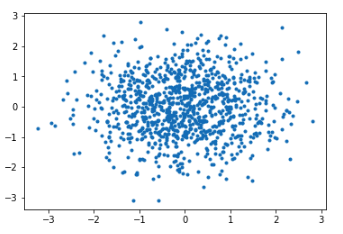
\includegraphics[height=5cm,width=7cm]{image/gaussdistribution} }}%
    \qquad
    \subfloat[Gaussian Distribution to bouding box]{{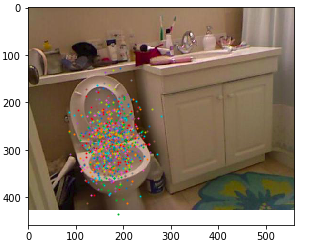
\includegraphics[height=5cm,width=7cm]{image/map_gaudis} }}%
    \caption{ \small a) Kết quả khởi tạo ngẫu nhiên  điểm theo phân bố Gaussian $ X_{random} \sim  N( \mu = (0,0),\sigma ^{2} = 1 )$.\\ b) Kết quả chuyển đổi tọa độ các điểm phân bố đến bao đóng vật thể 
    }
    \label{fig:gaussian_to_bbbox}%
\end{figure}

 
\subsection{Ước lượng khoảng cách dựa trên kết quả phân đoạn của Mask RCNN}
Dựa vào kết quả phân đoạn của Mask RCNN, ta sẽ có những điểm mà Mask RCNN cho là thuộc về vật thể. Kết hợp những điểm này với kết quả ảnh độ sâu từ FCRN, ta sẽ có giá trị độ sâu của tất cả những điểm thuộc về vật thể. Từ đây, lấy giá trị trung bình của tất cả những điểm trên làm giá trị khoảng cách vật thể.


\subsection{Ước lượng khoảng cách bằng cách lấy mẫu những điểm xung quanh tâm bao đóng của vật thể theo phân phối Gaussian, trong đó những điểm này phải được Mask RCNN cho là thuộc về vật thể}
Từ phương án 2, nhóm đã có danh sách những điểm thuộc về bao đóng vật thể, những điểm mà được chuyển đổi từ phân bố Gaussian. Trong những điểm này, nhóm chỉ lấy những điểm mà Mask RCNN cho là thuộc về vật thể. Sau khi có tập những điểm cuối cùng, lấy giá trị độ sâu của những điểm này từ ảnh độ sâu, và tiến hành tính giá trị khoảng cách bằng giá trị trung bình. 



% Qua quá trình tìm hiểu về các mô hình nhận diện vật thể, nhóm quyết định tìm hiểu sâu hơn về mô hình Faster R-CNN. Hiện tại, nhóm tham khảo và đang tiến hành nghiên cứu và chạy Faster R-CNN với mô hình VGG16 trên tập dữ liệu NYUV2 để tiến hành phát hiện vật thể. \\

% Với tập dữ liệu PASCALVOC2007 và mô hình VGG16 đã được huấn luyện sẵn, kết quả của bao đóng vật thể cho kết quả rất tốt.

% \begin{figure}[H]%
%     \centering
%     \subfloat[Detect person]{{\includegraphics[height=5cm,width=7cm]{image/example1} }}%
%     \qquad
%     \subfloat[Detect dog]{{\includegraphics[height=5cm,width=7cm]{image/example2} }}%
%     \caption{A cartoon drawing of a biological neuron (left) and its mathematical model (right).}%
%     \label{fig:example}%
% \end{figure}


% %chỗ này ta đang tiến hành train, trước mắt chưa có kết quả lập tức được. sẽ dán hình chỗ này sau.

% \section{Tiềm năng}

% Việc xác định vật thể trong không gian 3 chiều sẽ được ứng dụng vào trong nhiều lĩnh vực cũng như hệ thống, trong đó nổi bật nhất chính là phục vụ cho robot.
% \begin{itemize}
% \item Giúp robot có thể hiểu được kích cỡ vật thể, có thể tiến hành thao tác chính xác hơn.
% \item Với xe tự lái, khi có thể hiểu được ngữ cảnh 3 chiều, nó có thể biết được khoảng cách giữa các đối tượng để có thể tiến hành điều chỉnh hợp lí, phù hợp với tình trạng giao thông hiện tại.

% \end{itemize}

% \section{Khó khăn}

% Hiện tại, việc phát hiện vật thể trong không gian 2 chiều đã được nhóm tìm hiểu và đang tiến hành huấn luyện. Nhưng với mục tiêu có thể bao đóng vật thể trong không gian 3 chiều, nhóm vẫn còn gặp nhiều khó khăn.

% \begin{itemize}
% 	\item Nhóm có tìm hiểu các dataset về ảnh RGB-D như: SUN RGBD, NYUV2... và thấy NYUV2 khá tốt, đặc biệt đã có hiệu chỉnh về ảnh độ sâu. Về việc tự thu thập dữ liệu, ở đây là ảnh RGB-D bằng máy Kinect, nhóm vẫn chưa tìm hiểu cũng như tiến hành chụp ảnh. Ngoài ra, ảnh độ sâu thu được cũng thường bị nhiễu và cần phải điều chỉnh, tăng chất lượng của ảnh. 
%     \item Các bài báo nói về việc thực hiện bao đóng vật thể trong không gian 3 chiều khá khó hiểu, đồng thời đòi hỏi nhiều kiến thức khá phức tạp. Do vậy, nhóm còn khá mập mờ về phần này. Trong giai đoạn luận văn, nhóm sẽ cố gắng tìm hiểu kĩ hơn cũng như tham khảo ý kiến của thầy hướng dẫn để có thể hoàn thành mục tiêu của đề tài.
%     \item Về tài nguyên cho việc huấn luyện để thực hiện phát hiện vật thể trong không gian 2 chiều, hiện tại, nhóm đang tự huấn luyện bằng CPU để có thể dễ tiến hành điều chỉnh nên tốc độ huấn luyện khá chậm. Trong thời gian tới, nếu kết quả huấn luyện trên CPU khả quan hơn,  nhóm sẽ tiến hành huấn luyện trên tài nguyên mà thầy hướng dẫn cung cấp.
% \end{itemize}
% \section{Định hướng luận văn}
% Trong giai đoạn luận văn, nhóm sẽ tiến hành các công việc sau:
% \begin{itemize}
% \item Xác định rõ ràng hướng tiếp cận của nhóm.
% \item Thu thập dữ liệu từ máy Kinect, điều chỉnh dữ liệu, kết hợp với NYUV2 dataset.
% \item Hoàn thiện việc phát hiện vật thể trong không gian 2 chiều với dataset của nhóm.
% \item Tiến hành nghiên cứu nhiều hơn để có thể hiểu việc phát hiện vật thể trong không gian 3 chiều.
% \item Hiện thực mô hình để có thể phát hiện vật thể trong không gian 3 chiều.
% \end{itemize}


\chapter{Đánh giá kết quả}

Một trong những nhiệm vụ quan trọng của việc huấn luyện là tiến hành đánh giá kết quả thu được. Việc đánh giá kết quả nhằm mục đích phân tích, đánh giá hiệu quả của các mô hình. Nhóm sẽ tiến hành đánh giá mô hình FCRN, đây là mô hình sinh depth map mà nhóm sử dụng để ước lượng khoảng cách. Bên cạnh đó, nhóm cũng sẽ tiến hành đánh giá kết quả của việc ước lượng khoảng cách vật thể dựa trên 2 cách tiếp cận mà nhóm đã đề xuất. Dựa vào các kết quả thu được, nhóm sẽ đưa ra các nhận xét, đề cập các nhược điểm mô hình gặp phải và đưa ra phương pháp điều chỉnh trong quá trình sinh ra depth map cũng như ước lượng khoảng cách vật thể. 

\section{Các chuẩn đo được dùng để đánh giá mô hình}

\subsection{Các chuẩn đo để đánh giá mô hình sinh depth map}

Trong việc đánh giá kết quả của mô hình FCRN nói riêng, hay các cấu trúc khác của mô hình sinh depth map, thì theo khảo sát của nhóm, các độ đo thường được sử dụng: root mean squared error(RMSE), mean absolute relative error(REL)  Thresholded accuracy\\ 


Dưới đây là những độ đo đánh giá về độ lỗi của mô hình, tại đó $y_i$ là giá trị thực tế ta có, còn $y_i^{*}$ là giá trị dự đoán từ mô hình, và $\left | T \right |$ là tổng số điểm ảnh trên toàn bộ những bức ảnh được đánh giá.
\begin{itemize}
\item RMSE: $\sqrt[]{\frac{1}{\left | T \right |} \sum _{y\in T}\left \|y_{i}-y_{i}^{*}  \right \|^{2}}$\\
Độ đo này còn có tên khác standard deviation of residuals, nó dùng để đánh giá độ sai biệt trung bình giữa giá trị dự đoán từ mô hình so với giá trị thực tế. Nếu giá trị này càng nhỏ thì độ chênh lệch trung bình giữa giá trị dự đoán với giá trị thực tế càng nhỏ, điều đó cho thấy mô hình dự đoán càng tốt.
%\item Root mean squared error log (rmslog): $\sqrt[]{\frac{1}{\left | T \right |} \sum _{y\in T}\left \|\log y_{i}- \log y_{i}^{*}  \right \|^{2}}$

\item Mean absolute relative error (rel): $\frac{1}{\left | T \right |} \sum _{y\in T} \left | y_i - y_i^{*} \right |/y_i$\\
Mặc dù đã có độ đo rms nhưng độ đo này nói lên giá trị trung bình của tỉ lệ độ chênh lệch giữa giá trị dự đoán $y^{*}$ và giá trị thực tế y so với giá trị thực tế y có nghĩa rằng ngoài việc biết được sự chênh lệch trung bình giữa giá trị dự đoán với giá trị thực tế  từ rms, ta còn muốn biết trung bình thì độ chênh lệch này so với giá trị thực tế là bao nhiêu lần.

\item Mean $\log_{10}$ error (log10): $\frac{1}{\left | T \right |} \sum _{y\in T}\left | \log_{10}y_i- \log_{10}y_i^{*}  \right |$\\
 Bời vì $\left | \log_{10}y_i- \log_{10}y_i^{*}  \right | = \left | \log_{10}\frac{y_i}{y_i^{*}}  \right |$ do đó độ đo này cho biết trung bình thì giá trị tỉ lệ của độ sâu dự đoán và độ sâu thực tế ở dạng $log_{10}$.
\end{itemize}

Để đánh giá độ chính xác của mô hình sinh depth map ta dùng độ chính xác theo ngưỡng (accuracy with threshold):\\
\begin{itemize}
\item Relative error: $\max \left \{ \frac{y_i^{*}}{y_i}, \frac{y_i}{y_i^{*}} \right \}$\\
Độ lỗi này được dùng để đánh giá xem giá trị độ sâu mà mô hình dự đoán có chính xác hay không tùy thuộc vào ngưỡng mà ta cho trước. Cụ thể, với mỗi giá trị độ sâu được dự đoán ta sẽ có được độ lỗi theo relative error, nếu giá trị này nhỏ hơn theo giá trị của ngưỡng cho trước $\delta$ thì ta xem mô hình đã dự đoán chính xác độ sâu tại điểm ảnh đó.

%Đ tỉ lệ của $y^{i} $, $\max(\frac{y_i}{y_i^{*}},\frac{y_i^{*}}{y_i}) = \delta^{k} < threshold$ với k = 1, 2, 3\\
\item $\delta_i$: là phần trăm của những điểm ảnh mà mô hình đã dự đoán chính xác độ sâu so với tất cả những điểm mà mô hình đã đưa ra dự đoán, cụ thể ta có công thức sau,
 \begin{center}
 $\delta_i = \frac{\mathbf{card}\left ( \left \{ y_i^{*}:  \max \left \{ \frac{y_i^{*}}{y_i}, \frac{y_i}{y_i^{*}} \right \}  < 1.25^{i} \right \} \right )}{\mathbf{card}\left ( \left \{ y_i \right \} \right )}$
 \end{center}
 Ở đây $\mathbf{card}$ là số lượng phần tử của tập hợp, và ngưỡng của  độ chính xác $\delta_i$ là $1.25^{i}$. Các công trình mà nhóm khảo sát thường chọn 3 độ chính xác để đánh giá mô hình với i tương ứng là 1, 2 và 3
\end{itemize}
\subsection{Các chuẩn đo để đánh giá kết quả của việc ước lượng khoảng cách}
Khác với việc đánh giá kết quả dựa trên ground truth, thì việc ước lượng khoảng cách của nhóm sẽ dựa trên việc so sánh 2 cách tiếp cận khác nhau mà nhóm đã đề xuất. Những đánh giá sơ bộ của nhóm dựa trên các giá trị: min, max, mean, standard deviation.

\section{Đánh giá kết quả}
\subsection{Đánh giá kiến trúc của mô hình ước lượng độ sâu}

Để đánh giá kiến trúc của mô hình ước lượng độ sâu, nhóm sẽ tiến hành khảo sát sự ảnh hưởng của những hàm mất mát khác nhau, những kiến trúc decoder khác nhau dựa trên độ chính xác của kết quả dự đoán ảnh độ sâu trên tập xác thực

\begin{enumerate}
\item Hàm mất mát: Để đánh giá hiệu quả của các hàm mất mát, nhóm đã sử dụng cùng một kiến trúc, ở đây với decoder là lớp deconvolution kernel size $2x2$. Các hàm mất mát được nhóm đánh giá bao gồm: hàm $L_1$, $L_2$, berHu.
\begin{table}[H]
\centering
\begin{tabular}{ |p{1.5cm}|p{1.5cm}|p{1.5cm}|p{1cm}|p{1cm}|p{1cm}|p{1cm}|p{1cm}|p{1cm}|}
% \hline
% \multicolumn{3}{|c|}{Country List} \\|p{1cm}
\hline
Loss & Encoder &  Decoder & RMSE &  REL & log10 & $\delta_1$ & $\delta_2$ & $\delta_3$ \\
\hline
$L_1$ & Conv & Deconv2 & 0.652 & 0.196 & nan & 69.6 & 92.4 & 98.1 \\
\hline
$L_2$ & Conv &  Deconv2  & 0.717 & 0.229 & 0.093 & 62.2 & 89.6 & 97.3\\
\hline
berHu & Conv & Deconv2 & 0.633 & 0.195 & 0.079 & 70.8 & 92.7 & 98.1 \\
\hline
\end{tabular}
\caption{Sự ảnh hưởng từ các hàm mất mát đến kết quả dự đoán}
\label{tab:compare_loss}
\end{table}
Từ kết quả trên ta thấy hàm mất mát berHu cho kết quả tốt hơn 2 hàm còn lại, nên nhóm sẽ chọn hàm berHu là hàm mất mát cho quá trình huấn luyện từ đây trở về sau. Chúng ta cần chú ý giá trị nan ở độ lỗi log10 của $L_1$ gây ra là do mô hình đã dự đoán một giá trị khoảng cách âm tại một điểm ảnh nào đó nên kết quả độ lỗi log10 toàn cục là nan.
\item Kiến trúc decoder: Dựa vào kết quả của bảng \ref{tab:compare_loss}, nhóm đã chọn được hàm mất mát. Tiếp theo, từ những decoder đã được đề xuất, bao gồm: deconvolution 2, deconvolution 3, upconvolution và upprojection, nhóm sẽ tiến hành đánh giá và chọn ra decoder cho kết quả tốt nhất. Từ kết quả ở bảng \ref{tab:compare_decoder} ta thấy Deconv3 có kích thước kernel là $3\times3$ cho kết quả khá tương tự Deconv2 có kích thước kernel $2\times2$, đồng thời Upproj có vẻ tốt hơn một ít so với Upconv và bọn chúng tốt hơn hẳn Deconv3 và Deconv2, nên nhóm đi đến quyết định chọn kiến trúc Upproj làm kiến trúc cho bộ decoder cho những thí nghiệm trở về sau.

\begin{table}[H]
\centering
\begin{tabular}{ |p{1.5cm}|p{1.5cm}|p{1.5cm}|p{1cm}|p{1cm}|p{1cm}|p{1cm}|p{1cm}|}
% \hline
% \multicolumn{3}{|c|}{Country List} \\
\hline
Encoder &  Decoder & RMSE &  REL & log10  &$\delta_1$ & $\delta_2$ & $\delta_3$ \\
\hline
Conv & Deconv2 & 0.633 & 0.195 & 0.078 & 70.8 & 92.7 & 98.1 \\
\hline
 Conv &  Deconv3  & 0.632 & 0.196 & 0.079 &  70.2 & 92.7 & 98.1\\
\hline
 Conv & Upconv & 0.607 & 0.185 & 0.075 & 72.6 & 93.6 & 98.3 \\
\hline
Conv & Upproj & 0.606 & 0.182 & 0.075 & 72.6 & 93.3 & 98.4 \\
\hline
\end{tabular}
\caption{Sự ảnh hưởng của các decoder tới kết quả dự đoán}
\label{tab:compare_decoder}
\end{table}
% phải gõ thêm để hoàn thiện 
\end{enumerate} 

\subsection{Đánh giá kết quả ước lượng độ sâu}
Từ kết quả của việc đánh giá các hàm mất mát cũng như kiến trúc decoder của mô hình, nhóm sẽ tiến hành khảo sát sự ảnh hưởng của số lượng mẫu độ sâu lên chất lượng của kết quả dự đoán ảnh độ sâu. Nhóm sẽ tiến hành thử nghiệm với số mẫu tăng dần từ 0, 100, 200, 500, 700, 800, 1000, 2000, 3000, 5000. 
Sau khi chọn được hàm mất mát là berHu và kiến trúc decoder là Upprojection phục vụ cho quá trình huấn luyện. Nhóm sẽ tiến hành khảo sát sự ảnh hưởng của số lượng mẫu độ sâu lên chất lượng của kết quả dự đoán của mô hình, 


\begin{enumerate}
\item Deconvolution 2: mô hình sử dụng decoder là  deconvolution 2, hàm loss l1. Nhóm sẽ tiến hành thử nghiệm với các giá trị sampling depth khác nhau. 
% \begin{center}
\begin{table}[H]
\centering
\begin{tabular}{ |p{3cm}|p{1.5cm}|p{1.5cm}|p{1cm}|p{1cm}|p{1cm}|p{1cm}|   }
% \hline
% \multicolumn{3}{|c|}{Country List} \\
\hline
Mô hình & RMSE &  REL & log10 & $\delta_1$ & $\delta_2$ & $\delta_3$ \\
\hline
RGB & 0.621 & 0.186 & 0.076 & 72.7 & 93.0 & 98.2 \\
\hline
RGB+100 mẫu & 0.362 &  0.089  & 0.038 & 92.1 & 98.4 & 99.6\\
\hline
RGB+200 mẫu & 0.305 & 0.076 & 0.032 & 94.4 & 99.0 & 99.8 \\
\hline
RGB+500 mẫu & 0.290 & 0.071 & 0.030 & 95.0 & 99.2 & 99.8\\
\hline
RGB+700 mẫu & 0.280 & 0.068 & 0.029 & 95.4 & 99.3 & 99.8\\
\hline
RGB+800 mẫu & 0.304 & 0.074 & 0.032 & 94.9 & 99.2 & 99.8\\
\hline
RGB+1000 mẫu & 0.279 & 0.068 & 0.029 & 95.4 & 99.2 & 99.8\\
\hline
RGB+2000 mẫu & 0.284 & 0.069 & 0.029 & 95.5 & 99.3 & 99.8\\
\hline 
RGB+3000 mẫu & 0.282 & 0.068 & 0.029 & 95.7 & 99.4 & 99.9\\
\hline
RGB+5000 mẫu & 0.268 & 0.065 & 0.028 & 95.8 & 99.3 & 99.9\\
\hline
RGB+10000 mẫu & 0.261 & 0.064 & 0.027 & 96.0 & 99.4 & 99.9\\
\hline
\end{tabular}
\caption{So sánh kết quả trong kết quả mô hình sử dụng decoder deconvolution}
\label{tab:deconv2}
\end{table}
% \end{center}
% \includegraphics[width=\paperwidth,height=\textheight]{image/deconv2_s200}
 \begin{center}
   \begin{figure}[H]
   \begin{center}
   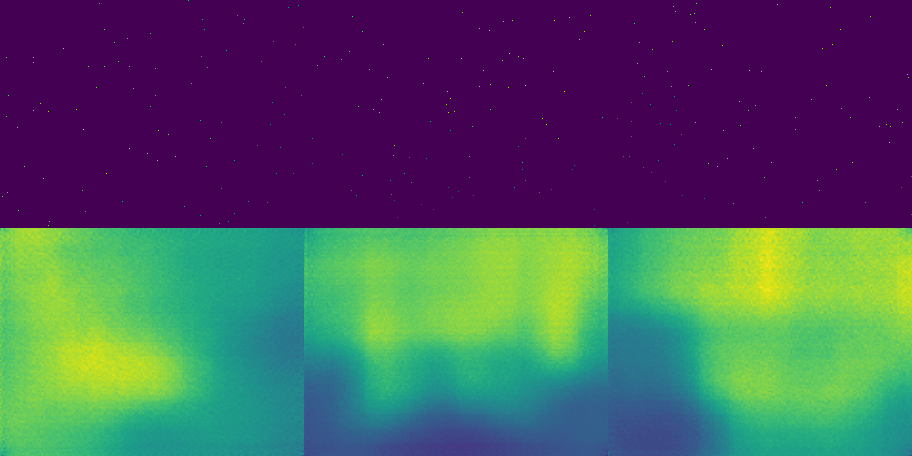
\includegraphics[scale=0.5]{image/100sample}
% \includegraphics[width=\paperwidth,height=\textheight]{image/deconv2_s200}
   \end{center}
   \caption[Kết quả so sánh khi dự đoán ảnh độ sâu với 200 điểm sampling dùng deconvolution 2]{Kết quả so sánh khi dự đoán ảnh độ sâu với 200 điểm sampling dùng deconvolution 2. Ảnh trong cột đầu tiên mô tả ảnh gốc RGB, ảnh thưa được thể hiện ở cột thứ 2. Trong cột thứ 3 và thứ 4 lần lượt là ground truth ảnh độ sâu và ảnh độ sâu được dự đoán khi sử dụng mô hình}
   \label{fig:deconv2_s200}
   \end{figure}
 \end{center}
 
%  \begin{center}
%    \begin{figure}[H]
%    \begin{center}
%    \includegraphics[scale=0.5]{image/comparison_169}
%    \end{center}
%    \caption{Kết quả so sánh khi dự đoán ảnh độ sâu với 100 điểm sampling dùng deconvolution 2.}
%    \label{fig:deconv2_100s}
%    \end{figure}
%  \end{center}
 
 \begin{center}
   \begin{figure}[H]
   \begin{center}
   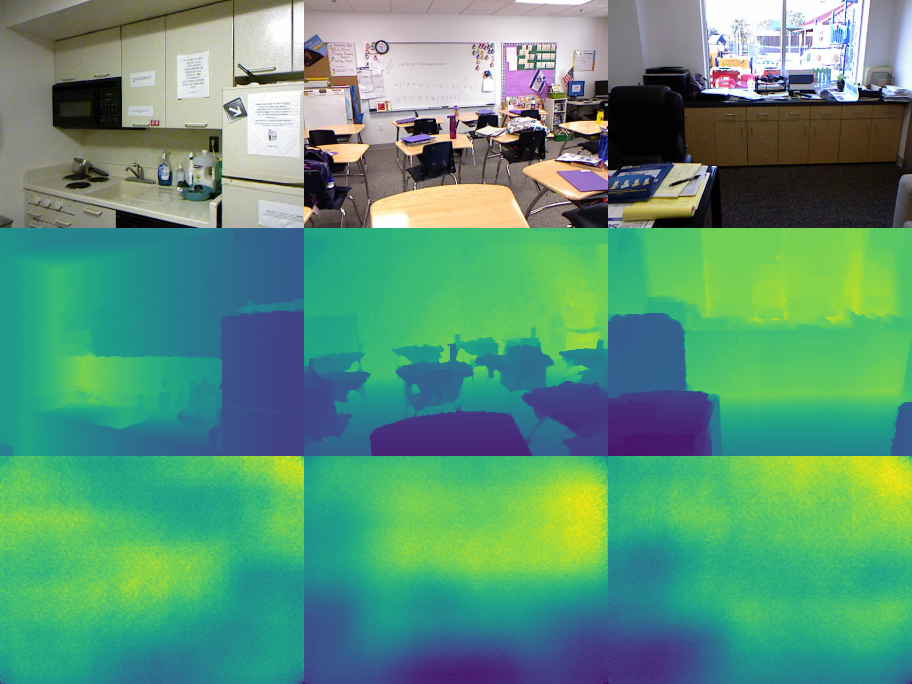
\includegraphics[scale=0.5]{image/0sample}
   \end{center}
   \caption[abcdef]{Kết quả so sánh khi dự đoán ảnh độ sâu với chỉ từ ảnh RGB dùng deconvolution 2}
   \label{fig:deconv2_0s}
   \end{figure}
 \end{center}

\item Deconvolution 3: mô hình sử dụng decoder là  deconvolution 3, hàm loss l1. Nhóm sẽ tiến hành thử nghiệm với các giá trị sampling depth khác nhau. 
% \begin{center}
\begin{table}[H]
\centering
\begin{tabular}{ |p{4cm}|p{2.5cm}|p{2cm}|p{1cm}|p{1cm}|p{1cm}|   }
% \hline
% \multicolumn{3}{|c|}{Country List} \\
\hline
Mô hình & RMSE &  REL & $\delta_1$ & $\delta_2$ & $\delta_3$ \\
\hline
Deconv3+0 sampling & 0.764 & 0.188 & 0.696 & 0.9492 & 0.9879 \\
\hline
Deconv3+100sampling & 0.483 &  0.103  & 0.895 & 09.9767 & 0.9947\\
\hline
Deconv3+200sampling & 0.447 & 0.093 & 0.918 & 0.9733 & 0.9937 \\
\hline
\end{tabular}
\caption{So sánh kết quả trong kết quả mô hình sử dụng decoder deconvolution 3}
\label{tab:deconv3}
\end{table}
 
 
 \item Upconvolution: mô hình sử dụng decoder là  upconvolution 3, hàm loss l1. Nhóm sẽ tiến hành thử nghiệm với các giá trị sampling depth khác nhau. 
% \begin{center}
\begin{table}[H]
\centering
\begin{tabular}{ |p{4cm}|p{2.5cm}|p{2cm}|p{1cm}|p{1cm}|p{1cm}|   }
% \hline
% \multicolumn{3}{|c|}{Country List} \\
\hline
Mô hình & RMSE &  REL & $\delta_1$ & $\delta_2$ & $\delta_3$ \\
\hline
Upconv+0 sampling & 0.808 & 0.198 & 0.604 & 0.9492 & 0.9879 \\
\hline
Upconv+100sampling & 0.461 &  0.099  & 0.902 & 09.9767 & 0.9947\\
\hline
Upconv+200sampling & 0.431 & 0.096 & 0.912 & 0.9733 & 0.9937 \\
\hline
\end{tabular}
\caption{So sánh kết quả trong kết quả mô hình sử dụng decoder upconvolution}
\label{tab:upconv}
\end{table}
 

\item Upprojection: mô hình sử dụng decoder là  upprojection, hàm loss l1. Nhóm sẽ tiến hành thử nghiệm với các giá trị sampling depth khác nhau. 
% \begin{center}
\begin{table}[H]
\centering
\begin{tabular}{ |p{4cm}|p{2.5cm}|p{2cm}|p{1cm}|p{1cm}|p{1cm}|   }
% \hline
% \multicolumn{3}{|c|}{Country List} \\
\hline
Mô hình & RMSE &  REL & $\delta_1$ & $\delta_2$ & $\delta_3$ \\
\hline
Upproj+0 sampling & 0.948 & 0.237 & 0.575 & 0.9492 & 0.9879 \\
\hline
Upproj+100sampling & 0.484 &  0.111  & 0.883 & 09.9767 & 0.9947\\
\hline
Upproj+200sampling & 0.496& 0.113 & 0.883 & 0.9733 & 0.9937 \\
\hline
\end{tabular}
\caption{So sánh kết quả trong kết quả mô hình sử dụng decoder upprojection}
\label{tab:upproj}
\end{table}
 
\end{enumerate}

\subsection{Đánh giá giá trị khoảng cách}
Các cách ước lượng khoảng cách vật thể mà nhóm đã đề xuất chủ yếu dựa trên kinh nghiệm, đồng thời, khoảng cách của những đối tượng trong ảnh đến camera cũng không được đánh nhãn. Do đó, nhóm chỉ có thể tiến hành đánh giá, so sánh các giá trị khoảng cách giữa các phương pháp với nhau. Các cách ước lượng khoảng cách mà nhóm đã hiện thực: lấy mẫu những điểm xung quanh tâm bao đóng của vật thể theo phân bố Gaussian ($all\_rdp$), lấy tất cả những điểm là kết quả của phân đoạn bằng Mask RCNN ($all\_mask$), lấy tất cả những điểm phân bố ngẫu nhiên thuộc kết quả phân đoạn Mask RCNN ($rdp\_mask$). \\ 

Từ tập dữ liệu NYUV2, nhóm chỉ chọn các hình ảnh có chứa những đối tượng: chai nước, giường ngủ và toi-let. Khi áp dụng mô hình FCRN và Mask RCNN trên tập ảnh này, nhóm thu được khoảng cách của 971 đối tượng bao gồm cả 3 loại trên. \\

% \begin{enumerate}[noitemsep]
\hspace{.2cm}\textbf{1. Tiến hành đánh giá sự chênh lệch khoảng cách của các phương pháp}: dựa trên khoảng cách đạt được từ ảnh độ sâu thực tế và ảnh độ sâu được dự đoán qua mô hình FCRN. Việc đánh giá sẽ tiến hành trên các đoạn khoảng cách khác nhau, bao gồm: 0 đến 1m, 1m đến 2m, 2m đến 3m, 3m đến 4m, 4m đến 5m, và lớn hơn 5m. Ví dụ: có khoảng 35 đối tượng nằm trong khoảng cách từ 0->1m(lấy dựa trên khoảng cách lấy được từ ảnh độ sâu thực tế). Từ đó, tính ra độ chênh lệch của những đối tượng đó giữa khoảng cách từ ảnh độ sâu thực tế và ảnh độ sâu được dự đoán và lấy giá trị trung bình của những giá trị chênh lệch này. 
\begin{table}[H]
\centering
\begin{tabular}{ |p{3cm}|p{1.5cm}|p{1.5cm}|p{1.5cm}|p{1.5cm}|p{1.5cm}|p{1.5cm}|}
% \hline
% \multicolumn{3}{|c|}{Country List} \\
\hline
PP đánh giá & 0-1m &  1-2m & 2-3m & 3-4m & 4-5m & >5m \\
\hline
$All\_rdp$ & 0.126 & 0.102 & 0.103 & 0.180 & 0.312 & 0.397 \\
\hline
$All\_mask$ & 0.121 &  0.106  & 0.111 & 0.168 & 0.305 & 0.374\\
\hline
$Rdp\_mask$ & 0.132& 0.111 & 0.116 & 0.188 & 0.314  & 0.422\\
\hline
\end{tabular}
\caption{So sánh sự chêch lệch giữa khoảng cách từ ảnh độ sâu thực tế và ảnh được dự đoán theo từng phương pháp}

\label{tab:compare_gtpred}
\end{table}

Theo kết quả từ bảng \ref{tab:compare_gtpred}, có thể thấy sự chênh lệch khoảng cách vật thể trong ảnh độ sâu thực tế và ảnh dự đoán là dựa vào độ chính xác của việc dự đoán ảnh độ sâu. Với những vật nằm ở khoảng cách càng xa camera, sự chính xác trong việc dự đoán ảnh độ sâu càng giảm, dẫn tới sự chênh lệch trong việc dự đoán khoảng cách vật thể từ ảnh độ sâu thực tế và ảnh độ sâu dự đoán là càng lớn. Bên cạnh đó, từ kết quả của bảng trên, nhóm cũng thấy rằng khi vật thể nằm trong khoảng từ 1-3 mét, sự chênh lệch của việc dự đoán khoảng cách từ ảnh độ sâu thực tế và ảnh độ sâu dự đoán là nhỏ nhất. Mặt khác, nếu vật ở quá gần camera, chẳng hạn như đoạn 0-1m, thì sự chênh lệch của khoảng cách lại lớn hơn so với đoạn từ 1-3m . Hình \ref{fig:deviation} thể hiện trực quan sự thay đổi của độ chênh lệch khoảng cách giữa ảnh độ sâu thực tế và ảnh độ sâu dự đoán của các phương pháp đo khoảng cách mà nhóm đề xuất.  

\begin{center}
   \begin{figure}[H]
   \begin{center}
   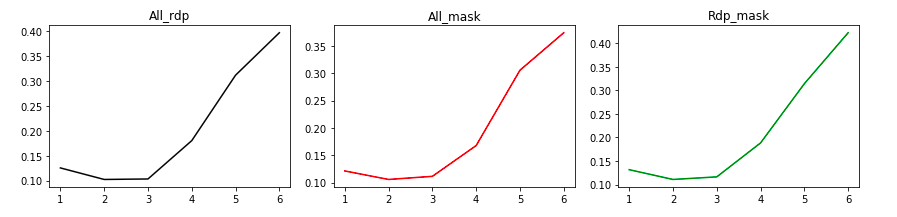
\includegraphics[scale=0.55]{image/deviation}
   \end{center}
   \caption{Sự chênh lệch khoảng cách giữa ảnh độ sâu thực tế và ảnh dự đoán}
   \label{fig:deviation}
   \end{figure}
 \end{center}
 
 Các giá trị trong bảng \ref{tab:compare_gtpred} là giá trị trung bình của sự chênh lệch khoảng cách thuộc đoạn, do đó giá trị trên là khá lớn vì trong mỗi đoạn đều sẽ chứa những nhiễu gây ảnh hưởng đến giá trị mà ta thu được. Hình \ref{fig:distribution} thể hiện rõ hơn sự phân bố của những giá trị chênh lệch này. Nhóm đã tiến hành đếm số lượng sự chênh lệch khoảng cách giữa ảnh độ sâu thực tế và ảnh dự đoán.  Ví dụ, trong phương pháp $all\_rdp$ có khoảng 221 độ chênh lệch khoảng cách nằm trong đoạn từ 0m đến 0.03m, khoảng 183 độ chênh lệch khoảng cách cách nằm trong đoạn từ 0.03m đến 0.06m... \\
 
 Từ đây, nhóm thấy rằng sự chênh lệch các giá trị khoảng cách là không quá lớn, đa số các độ chênh lệch tập trung vào khoảng sai số từ 0m đến 0.2m.Tuy nhiên, vẫn có một vài trường hợp cho ta thấy sự chênh lệch khá lớn. Một trong những lý do chính có thể dẫn đến sự chênh lệch này có thể là do kết quả dự đoán ảnh độ sâu có sự sai khác lớn đối với ảnh thực tế.
 \begin{center}
   \begin{figure}[H]
   \begin{center}
   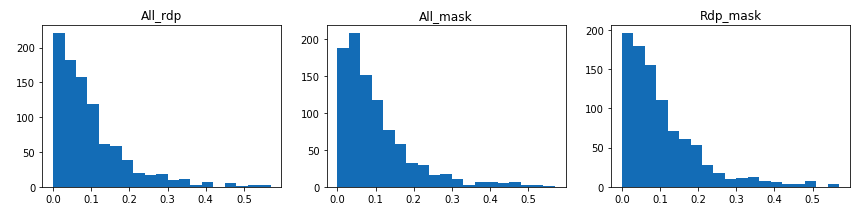
\includegraphics[scale=0.55]{image/distribution}
   \end{center}
   \caption{Sự chênh lệch khoảng cách giữa ảnh độ sâu thực tế và ảnh dự đoán}
   \label{fig:distribution}
   \end{figure}
 \end{center} 
 \hspace{.2cm}\textbf{2. Tiến hành đánh giá sự ảnh hưởng của hình dạng vật thể với kết quả dự đoán ảnh độ sâu}: những vật thể mà nhóm chọn để đánh giá bao gồm: chai nước, giường ngủ và toi-let. Mỗi vật thể trên đều có hình dáng rất khác nhau.\\
 
Nhóm đã chọn kết quả phân đoạn từ Mask RCNN làm kết quả bề mặt của vật thể  và tiến hành phân tích bằng cách chọn giá trị độ sâu lớn nhất và nhỏ nhất của những bề mặt vật thể này trên ảnh độ sâu thực tế. Sau đó tiến hành so sánh giữa độ chênh lệch của giá trị lớn nhất, giá trị nhỏ nhất này giữa từng loại vật thể. 


 
 


\newpage
% 
%  \begin{thebibliography}{80}
 
% \bibitem{rcnn}
% R. Girshick, J. Donahue, T. Darrell, and J. Malik, “Rich feature hierarchies for accurate object detection and semantic segmentation,” in IEEE Conference on Computer Vision and Pattern Recognition (CVPR), 2014.
% \bibitem{fastrcnn}
% R. Girshick, “Fast R-CNN,” in IEEE International Conference on Computer Vision (ICCV), 2015.
% \bibitem{fasterrcnn}
%  S. Ren, K. He, R. Girshick, and J. Sun.  Faster R-CNN: Towards  real-time  object  detection  with  region  proposal  networks. In NIPS, 2015.
%  \bibitem{maskrcnn}
%  K. He, G. Gkioxari, P. Dollar, and R. B. Girshick. Mask R-CNN, in ICCV, 2017.
%  \bibitem{fcrn}
%  I. Laina, C. Rupprecht, V. Belagiannis, F. Tombari, andN. Navab. Deeper depth prediction with Fully Convolutional Residual Networks. In 3D Vision (3DV), 2016 Fourth International Conference on, pages 239–248. IEEE, 2016.
 
% \bibitem{DLbook}
% (Adaptive Computation and Machine Learning series) Bengio, Yoshua Courville, Aaron Goodfellow, Ian J-Deep learning adaptive computation and machine learning-The MIT Press (2016).
% \bibitem{cs231n}
%  CS231n Convolutional Neural Networks for Visual Recognition
% \bibitem{kinect}
%  Leandro Cruz, Djalma Lucio, Luiz Velho. Kinect and RGBD Images: Challenges and Applications. In IEEE, 2012.
% \bibitem{amodal3dobject}
% Z. Deng and L. J. Latecki. Amodal detection of 3d objects: Inferring 3D bounding boxed from 2D ones in RGB-Depth images. In CVPR. 2017.
% \bibitem{learningrichfeature}
% S. Gupta, R. Girshick, P. Arbeláez, and J. Malik. Learning rich features from RGB-D images for object detection and segmentation. In European Conference on Computer Vision, pages 345–360. Springer, 2014.
% \bibitem{MCG}
% P. Arbeláez, J. Pont-Tuset, J. T. Barron, F. Marques, and J. Malik. Multiscale combinatorial grouping. In Proceedings of the IEEE Conference on Computer Vision and Pattern Recognition, pages 328–335, 2014.
% \bibitem{toward}
% W. Liu, R. Ji, and S. Li. Towards 3d object detection with bimodal deep boltzmann machines over rgbd imagery. In CVPR. 2015.
% \bibitem{guppta}
% S. Gupta, P. Arbelaez, R. Girshick, and J. Malik. Aligning 3d models to rgb-d images of cluttered scenes. In CVPR. 2015.
% \bibitem{Kim}
% B. soo Kim, S. Xu, and S. Savarese. Accurate localization of 3d object from rgb-d data using segmentation hypothesis. In ICCV. 2013.
% \bibitem{ss}
% S. Song and J. Xiao. Sliding shapes for 3d object detection in depth images. In ECCV. 2014.
% \bibitem{three}
% Z. Ren and E. B. Sudderth. Three-dimensional object detection and layout prediction using clouds of oriented gradients.
% In CVPR. 2016.
% \bibitem{dss}
% S. Song and J. Xiao. Deep sliding shapes for amodal 3d object detection in rgb-d images. In CVPR. 2016.
% \bibitem{VGG}
% K. Simonyan and A. Zisserman. Very deep convolutional
% networks for large-scale image recognition. arXiv, 2014.
%  \end{thebibliography}

\bibliography{refs} 
\bibliographystyle{ieeetr}


%\bibliography{refs}{}
%\bibliographystyle{plain}
%-	Danh mục TL tham khảo
%-	Phụ lục (nếu có)

\end{document}
